\documentclass[10pt,journal,compsoc]{IEEEtran}
\usepackage{graphicx}
\usepackage{balance}  % for  \balance command ON LAST PAGE  (only there!)
\usepackage{enumitem}
\usepackage{rotating} % for tab
\newtheorem{myDef}{Definition}
\newtheorem{myTheo}{Theorem}

\usepackage[usenames,dvipsnames]{xcolor}

\newcommand{\TODO}[1]{\textcolor{red}{\textbf{[TODO:#1]}}}
\newcommand{\TODOREP}[1]{\textcolor{ForestGreen}{\textbf{[TODO:#1]}}}
\newcommand{\Z}{{\bf H-zkNNJ}}
\newcommand{\LSH}{{\bf RankReduce}}
\newcommand{\VO}{{\bf PGBJ}}
\newcommand{\HBNLJ}{{\bf H-BNLJ}}
\newcommand{\HBK}{{\bf H-BkNNJ}}

% *** CITATION PACKAGES ***
%
\usepackage{cite}
\usepackage{lscape}
\usepackage{color}

% *** sub***
%
\usepackage{caption}
\usepackage{subcaption}

\usepackage{multirow}

%to strike out text use \sout
\usepackage[normalem]{ulem}

%\usepackage{stfloats}

% *** MATH PACKAGES ***
%
%\usepackage[cmex10]{amsmath}
\usepackage{latexsym}
\usepackage{amssymb}
\usepackage{algorithmic}
\usepackage{array}
\usepackage{mdwmath}
\usepackage{mdwtab}
\usepackage{eqparbox}
\usepackage{caption}
\setlength\abovecaptionskip{1mm}
\setlength\belowcaptionskip{0mm}
\setlength{\textfloatsep}{5pt}
\usepackage{float}
\usepackage{hyperref}
\usepackage{boxedminipage}
\usepackage{mwe} % new package from Martin scharrer
\usepackage{authblk}

%\setlength{\topskip}{0pt}
\setlength{\topsep}{2pt}


% to strikeout
\usepackage[normalem]{ulem}


\newcommand\MYhyperrefoptions{bookmarks=true,bookmarksnumbered=true,
pdfpagemode={UseOutlines},plainpages=false,pdfpagelabels=true,
colorlinks=true,linkcolor={black},citecolor={black},urlcolor={black},
pdftitle={Bare Demo of IEEEtran.cls for Computer Society Journals},%<!CHANGE!
pdfsubject={Typesetting},%<!CHANGE!
pdfauthor={Michael D. Shell},%<!CHANGE!
pdfkeywords={Computer Society, IEEEtran, journal, LaTeX, paper,
             template}}%<^!CHANGE!



\begin{document}

\title{K Nearest Neighbour Joins for Big Data on MapReduce: a Theoretical and Experimental Analysis }


\author{\IEEEauthorblockN{Ge Song\IEEEauthorrefmark{2},
Justine Rochas\IEEEauthorrefmark{1}, Lea El Beze\IEEEauthorrefmark{1}, 
Fabrice Huet\IEEEauthorrefmark{1} and
Fr\'ed\'eric Magoul\`es\IEEEauthorrefmark{2}}
\newline \IEEEauthorblockA{\IEEEauthorrefmark{1}Univ. Nice Sophia Antipolis, CNRS, I3S, UMR 7271, 06900 Sophia Antipolis, France}
\newline \IEEEauthorblockA{\IEEEauthorrefmark{2}CentraleSup\'elec, Universit\'e Paris-Saclay, France
 \\
ge.song@ecp.fr, \{justine.rochas,  fabrice.huet\}@unice.fr}, lea.elbeze@gmail.com , frederic.magoules@hotmail.com
}

\IEEEtitleabstractindextext{
\begin{abstract}
Given a point $p$ and a set of points $S$, the kNN operation finds the $k$ closest points to $p$ in $S$. It is a computational
intensive task with a large range of applications such as knowledge discovery or data mining. However, as the volume
and the dimension of data increase, only distributed approaches can perform such costly operation in a reasonable time. 
Recent works have focused on implementing efficient solutions using the MapReduce programming model because it is suitable for 
distributed large scale data processing.  Although these works provide
different solutions to the same problem, each one has particular constraints and properties. 
In this paper, we compare the different existing approaches for computing kNN on MapReduce, first theoretically, and then by performing an extensive experimental evaluation. To be able to compare solutions, we identify three generic steps for kNN computation on MapReduce: data pre-processing, data partitioning and computation. We then analyze each step from load balancing, accuracy and complexity aspects. Experiments in this paper use a variety of datasets, and analyze the impact of data volume, data dimension and the value of k from many perspectives like time and space complexity, and accuracy. The experimental part brings new advantages and shortcomings that are discussed for each algorithm. To the best of our knowledge, this is the first paper that compares kNN computing methods on MapReduce both theoretically and experimentally with the same setting. Overall, this paper can be used as a guide to tackle kNN-based practical problems in the context of big data. 
\end{abstract}
\begin{IEEEkeywords}
kNN, MapReduce, Performance Evaluation
\end{IEEEkeywords}}
\maketitle
\IEEEdisplaynontitleabstractindextext
\IEEEpeerreviewmaketitle
\ifCLASSOPTIONcompsoc
\section{Introduction}
\IEEEPARstart{G}{iven} a set of query points $R$ and a set of reference points $S$, a $k$ nearest neighbor join 
(hereafter kNN join) is an operation which, for each point in $R$, discovers 
the $k$ nearest neighbors in $S$. 

It is frequently used as a classification or clustering method in machine learning or data mining. The primary 
application of a kNN join is k-nearest neighbor classification. Some data points are given for training, and some 
new unlabeled data is given for testing. The aim is to find the class label for the new points. For each unlabeled 
data, a kNN query on the training set will be performed to estimate its class membership. This process can be 
considered as a kNN join of the testing set with the training set. The kNN operation can also be used to identify
 similar images. To do that, description features (points in a dataspace of dimension 128) are first extracted from 
 images using a feature extractor technique. Then, the kNN operation is used to discover the points that are close, 
 which should indicates similar images. Later in this paper, we consider this kind of data for the kNN computation. kNN 
 join, together with other methods, can 
be applied to a large number of fields, such as multimedia 
\cite{knn_video_matting_iccv2013,Kriegel:1998:ASS:594718.594761}, social 
network \cite{Bai:2011:CPT:2043652.2043659}, time series analysis 
\cite{Rafiei:1997:SQT:253262.253264,Agrawal:1993:ESS:645415.652239}, bio-information and medical 
imagery \cite{5930107,Korn:1996:FNN:645922.673493}. 

The basic idea to compute a kNN join is to perform  a pairwise computation of distance for each element in $R$ and each 
element in $S$. The difficulties mainly lie in the following two aspect: (1)Data Volume (2)Data Dimensionality. 
Suppose we are in a d dimension space, the computational 
complexity of this pairwise calculation is $O(d \times \left|R\right| \times \left| S \right|)$. Finding the $k$ 
nearest neighbors in $S$ for every $r$ in $R$ 
boils down to finding the smallest $k$ distances, and leads to a minimum complexity of $\left| S \right| \times log 
\left| S \right|$. As the amount of data or their complexity (number of dimensions) increases, this approach becomes 
impractical. This is why a lot of work has been dedicated to reducing the in-memory 
computational 
complexity \cite{DBLP:journals/tods/JagadishOTYZ05_full,MuX_full,
Ciaccia:1997:MEA:645923.671005,DBLP:journals/geoinformatica/YuZHX10,
Bentley:1975:MBS:361002.361007}. These works mainly focus on two points: (1) Using indexes to decrease the number of 
distances need to be calculated. However, these indexes can hardly be scaled on high dimension data. (2) Using 
projections to reduce the dimensionality of data. But the maintenance of the accuracy becomes another problem. Despite 
these efforts, there are still significant limitations to process kNN on a single machine when the amount of data 
increases. For large dataset, only distributed and parallel solutions prove to be powerful enough. 
MapReduce is a flexible and scalable parallel and distributed programming paradigm which is specially designed for 
data-intensive processing. It was first 
introduced by Google \cite{Dean:2008:MSD:1327452.1327492} and popularized with the Hadoop framework, an open source 
implementation. 
The framework can be 
installed on commodity hardware and automatically distribute a MapReduce job over a set of machines. Writing an 
efficient kNN in MapReduce is also
challenging for many reasons. 
First, classical algorithms as well as the index and projection strategies have to be redesigned to fit the MapReduce 
programming model and its share-nothing execution platform. 
Second, data partition and distribution strategies have to be carefully designed to limit 
communications and data transfer. 
Third, the load balancing problem which is new comparing with the single version should also be attached importance to. 
Then, not only the number of distance needed to be reduced, but also the number of MapReduce jobs and map/reduce tasks 
will bring impact.
Finally, the parameter tuning remains always a key point to improve the performance.

The goal of this paper is to survey existing methods of kNN in MapReduce, and to compare their performance. It is a 
major extension of one of our previously published paper, \cite{song:hal-01097337}, which provided only a simple 
theoretical analysis. 
Other surveys about kNN have been conducted, such as \cite{SurveyNNTechniques,Jiang:2007:SIK:1302500.1303257}, but they 
pursue a different goal. In \cite{SurveyNNTechniques}, the authors 
only focus on centralized solutions to optimize kNN computation whereas we target distributed solutions. In 
\cite{Jiang:2007:SIK:1302500.1303257}, the 
survey is also oriented towards centralized techniques and is solely based on a theoretical performance analysis. Our 
approach comprehends both 
theoretical and practical performance analysis, obtained through extensive 
experiments. To the best of our knowledge, it is the first time such a comparison between existing kNN solutions on 
MapReduce has been performed. The breakthrough of this paper is that the solutions are experimentally compared in the 
same setting: same hardware and same dataset. 
Moreover, we present in this paper experimental settings and configurations that were not studied in the original 
papers.
Overall, our contributions are:
\begin{itemize}[noitemsep,nolistsep]
\item The decomposition of a distributed MapReduce kNN computation in different basic steps, introduced in Section~\ref{workflowsec}.
\item A theoretical comparison of existing techniques in Section~\ref{analysis}, focusing on load balancing, accuracy and complexity aspects.
\item An implementation of 5 published algorithms and an extensive set of experiments using both low and high dimension 
datasets (Section~\ref{evaluation}).
\item An analysis which outlines the influence of various parameters on the performance of each algorithm.
\end{itemize}
The paper is concluded with a summary that indicates the typical dataset-solution coupling and provides
precise guidelines to choose the best algorithm depending on the context.
%\section{Context}
%In this section, we introduce concepts needed throughout the rest of the paper. 
%the kNN operation and the MapReduce framework, as well as some needed concepts to compare the existing methods about kNN 
%joins.
\subsection{k Nearest Neighbors}
A nearest neighbors query consists in finding at most $k$ points in a data set $S$ that are the closest to a considered point $r$, in a dimensional space $d$. More formal definitions are as follows: 
%Here we will see some definitions about kNN in this part.
%\TODO{I am not happy with the bunch of definitions here, too many, do we really need all of them?}
given two data sets $R$ and $S$ in $\mathbf{R}^d$, and given $r$ and $s$, two elements, with $r \in R$ and $s \in S$, we have:
%
%\begin{myDef}
%	The \textbf{similarity distance} between any two elements is their distance $d(r,s)$.
%\end{myDef}

\begin{myDef}
	Let $d(r,s)$ be the distance between $r$ and $s$. The \textbf{kNN query} of $r$ over $S$, noted $kNN(r,S)$ is the subset $\{s_i\} \subseteq S$ $\left(\left|\{s_i\}\right| = k\right)$, which is the $k$ nearest neighbors of $r$ in $S$, where $\forall$ $s_i \in kNN(r,S)$, $\forall$ $s_j \in S-kNN(r,S)$, $d(r,s_i) \leq d(r,s_j)$.
\end{myDef}

It is easy to extend the previous definition to a set of query points. 
\begin{myDef}
	The \textbf{kNN join} of two datasets $R$ and $S$, kNN($R$ $\ltimes$ $S$) is:
	\begin{center}
	kNN($R$ $\ltimes$ $S$)=\{($r$,kNN($r$,$S$)), $\forall$ $r \in R$\}
	\end{center}	
\end{myDef}
Depending on the use case, it might not be necessary to find the exact solution of a kNN query, and that is why approximate kNN queries have been introduced. The idea is to have the $k^{th}$ approximate neighbor not far from the $k^{th}$ exact one, as shown in the following definition. 
\begin{myDef}
    The \textbf{$\left(1+\epsilon\right)$-approximate kNN query} for a query point $r$ in a dataset $S$, $AkNN(r,S)$ is a set of approximate $k$ nearest neighbors of $r$ from $S$, if the $k^{th}$ furthest result $s^{k*}$ satisfies $s^{k*} \leq s^k \leq (1+\epsilon)s^{k*} $ $(\epsilon > 0)$ where $s^k$ is the exact $k^{th}$ nearest neighbor of $r$ in $S$.
\end{myDef}

And as with exact kNN, this definition can be extended to an approximate kNN join. 
\begin{myDef}
    The \textbf{$\left(1+\epsilon\right)$-approximate kNN join} of two datasets $R$ and $S$, AkNN($R$ $\ltimes$ $S$) is:
	\begin{center}
	AkNN($R$ $\ltimes$ $S$)=\{($r$,AkNN($r$,$S$)), $\forall$ $r \in R$\}
	\end{center}	    
\end{myDef}


The basic solution to compute kNN adopts a block nested loop approach, which calculates the distance between every object $r_i$ in $R$ and $s_j$ in $S$ and 
sorts the results to find the $k$ smallest. This approach is computational intensive, making it unpractical for large or intricate datasets. Two
strategies have been proposed to work out this issue.  
%To overcome the limitation of this trivial method, many improvements have been done. These improvements can be divided into 2 categories:

The first one consists in reducing the number of distances to compute, by avoiding scanning the whole dataset. This strategy focuses on indexing the 
data through efficient data structures. For example, a one-dimension index structure, the $B^+$-Tree, is used in \cite{DBLP:journals/tods/JagadishOTYZ05} to index distances; 
\cite{MuX} adopts a multipage overlapping index structure R-Tree, whose minimum bound is a rectangle (MBR); \cite{Ciaccia:1997:MEA:645923.671005} 
proposes to use a balanced and dynamic M-Tree to organize the dataset; \cite{Yu:2010:HKJ:1713160.1713227} introduces a sphere-tree with a sphere-shaped minimum bound to reduce the number of areas to be searched; \cite{Andreica13sequentialand} presents a multidimensional quad-tree in order to be able to handle large 
amount of data; and \cite{Bentley:1975:MBS:361002.361007} develops a kd-tree which is a  clipping partition method to separate the search space.

%\end{itemize}

However, reducing the searched dataset might not be sufficient. For data in large dimension space, computing the distance might 
be very costly. That is why a second strategy focuses on projecting the high-dimension dataset onto a low-dimension one, while maintaining the 
locality relationship between data. Representative efforts refer to LSH (Locality-Sensitive Hashing) \cite{Datar:2004:LHS:997817.997857} and 
Space  Filling Curve \cite{5447837}.
In these cases, the low-dimension data contain much less information than the high-dimension ones
because in most cases, the low-dimension data cannot totally fill the high-dimension space. To keep as much information as possible, the trick is to project the high-dimension data multiple times from different perspectives, producing multiple new
datasets.
%\TODO{Done} So these projection methods usually perform multiple operations. 
For instance, LSH usually provides many space hashing functions. The space filling curve method also usually needs several shifts 
of data, to reduce the possibilities of errors in the data locality when projecting. 

But with the increasing amount of data, these methods can still not handle kNN computation 
on a single machine efficiently. Experiments in \cite{10.1371/journal.pone.0044000} suggest using GPUs to significantly improve the 
performance of distance computation, but this is still not applicable for large datasets that cannot reasonably be processed on a single machine. 

%Despite these improvements, large dataset cannot  reasonably be processed on a single machine. 
Recent papers have focused on providing efficient distributed implementations. Some of 
them use ad hoc protocols based on well-known distributed architectures \cite{Novak:2006:MSD:1146847.1146866,Haghani_lshat}. But most of them use the MapReduce model as it is naturally adapted for distributed computation, like in \cite{Stupar10rankreduce-,Lu:2012:EPK:2336664.2336674,Zhang:2012:EPK:2247596.2247602}. In this paper, we focus on the kNN computing systems based on MapReduce, because such systems can scale with the predictable data growth, and also because the framework on which they are based is widespread. 
%\TODO{TODO check phrase}

%
%Since all these improvements have limitations, and these limitations are caused by the amount or the dimension of data, it is indispensable to 
%implement these methods on a parallel and distributed framework such as MapReduce. There have already been some successful works of running kNN on top 
%of MapReduce. Zhang et. al. present an exact and an approximate way of processing kNN on MapReduce in their paper \cite{Zhang:2012:EPK:
%2247596.2247602}. Another similar work was introduced by Lu et. al. in \cite{Lu:2012:EPK:2336664.2336674}. RankReduce \cite{Stupar10rankreduce-} was 
%developed to propose an approach to implement LSH on top of MapReduce. And \cite{Andreica13sequentialand} adapt the well-known sequential algorithms to 
%MapReduce in order to find the nearest neighbors.

%\textit{TODO: definition plus formelle ?}
%The naive way to compute kNN join is, for each point in R to compute the distance from all points in S and keep the k ones for which the distance to the point in R is the smallest. This leads to a complexity O(|R| x |S|) which is not bearable for any real data sets.

\subsection{MapReduce}
MapReduce \cite{Dean:2008:MSD:1327452.1327492} is a parallel programming model that aims at efficiently processing large datasets. This programming 
model is based on three concepts: (i) representing data as key-value pairs, (ii) defining a map function, and (iii) defining a reduce function. 
The map function takes key-value pairs as an input, and produces zero or more key-value pairs. Outputs with the same key are gathered together (shuffled) so that key-\{list of values\} pairs are given to reducers. The reduce function processes all the values associated
with a given key. 
%The overall workflow of a MapReduce computation is shown in Figure~\ref{mapreduce_workflow}.

%\begin{figure*}[htp]
%\center
%\scalebox{0.4}{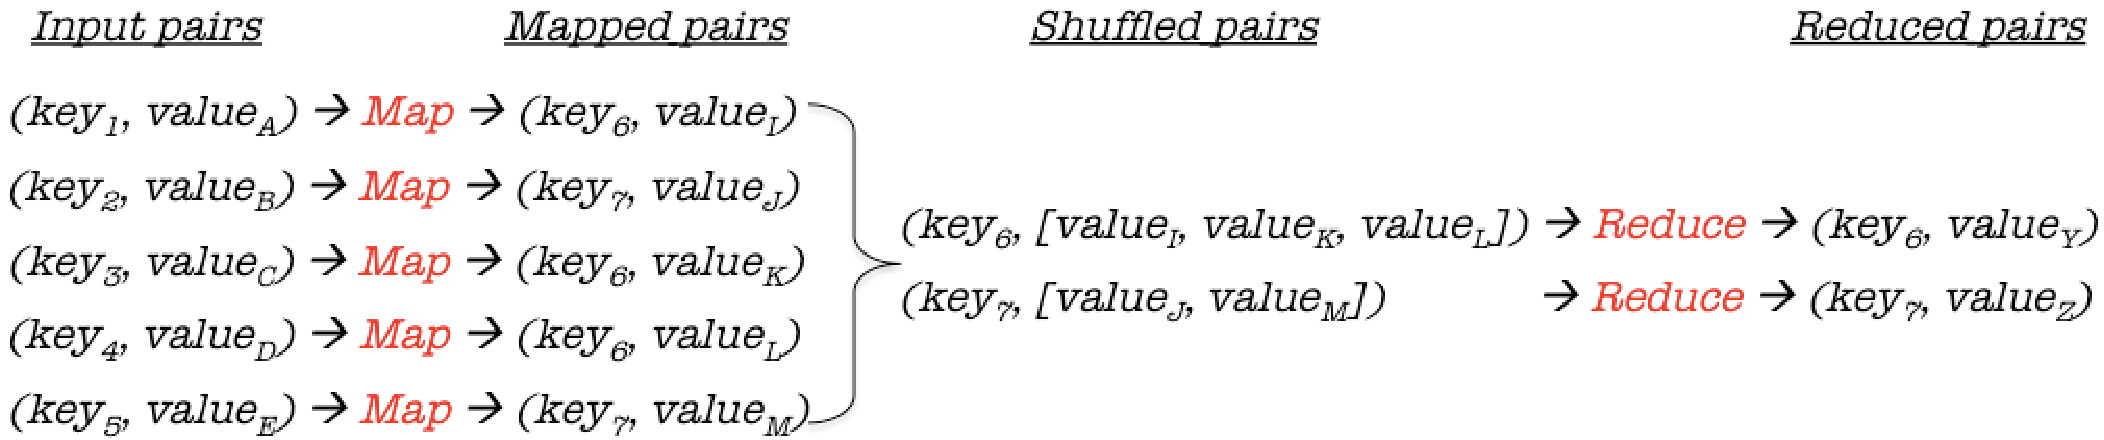
\includegraphics{res/mapreduce.pdf}}
%\caption{MapReduce workflow \label{mapreduce_workflow}}
%\end{figure*}

This decomposition enables data parallelism as the only dependency between the output of the maps and input of reduces. In 
practice, the map and reduce functions can be executed on many machines, leading to a naturally distributed computation. The most famous implementation
of this model is the Hadoop framework \cite{Hadoop:Website} which provides a distributed platform for executing MapReduce jobs. 
%This programming model is based on a representation of data as key-value pairs and on consecutive call of the map and reduce functions, that take as 
%parameter key-value pairs and that also return key-value pairs. The user of the framework has to provide the data format, and the body of the map and 
%reduce functions. The framework then handle parallel and join phases. Typically, massive map tasks (called Mapper) are triggered in parallel according 
%to the data format provided whereas reduce tasks (called Reducer) will gather and then process Mapper's output that have the same key to produce the 
%final output, as can be seen in Figure~\ref{mapreduce_workflow}. 

%\textit{- Distribution:} Many implementations of the MapReduce programming model are adapted to distribution, such as the Hadoop framework 
%\cite{Hadoop:Website}. Indeed, mappers usually process subsets of data that are independent from each other. It is thus natural to distribute mappers 
%across a set of machines, thereby scaling to terabytes of data to process. 

%\TODO{Not sure we need this, we have already justified the paper in the introduction. I suggest removing it}.
%In the context of this paper, using MapReduce to compute kNN join is 
%challenging in the sense that, to be efficient, the kNN query must be run for each point on a subset of the data rather than on the whole data set. It 
%is also a requirement to be compliant with the MapReduce model, since each part of the computation should be independent from each other. We will thus 
%review existing partitioning techniques to do that in the context of MapReduce, and also broader.
\section{Context}
\subsection{k Nearest Neighbors}
A nearest neighbors query consists in finding at most $k$ points in a data set $S$ that are the closest to a considered point $r$, in a dimensional space $d$. More formally, 
given two data sets $R$ and $S$ in $\mathbf{R}^d$, and given $r$ and $s$, two elements, with $r \in R$ and $s \in S$, we have:
\begin{myDef}
	Let $d(r,s)$ be the distance between $r$ and $s$. The \textbf{kNN query} of $r$ over $S$, noted $kNN(r,S)$ is the subset $\{s_i\} \subseteq S$ $\left(\left|\{s_i\}\right| = k\right)$, which is the $k$ nearest neighbors of $r$ in $S$, where $\forall$ $s_i \in kNN(r,S)$, $\forall$ $s_j \in S-kNN(r,S)$, $d(r,s_i) \leq d(r,s_j)$.
\end{myDef}
This definition can be extended to a set of query points:
\begin{myDef}
	The \textbf{kNN join} of two datasets $R$ and $S$, kNN($R$ $\ltimes$ $S$) is:
	kNN($R$ $\ltimes$ $S$)=\{($r$,kNN($r$,$S$)), $\forall$ $r \in R$\}	
\end{myDef}
Depending on the use case, it might not be necessary to find the exact solution of a kNN query, and that is why approximate kNN queries have been introduced. The idea is to have the $k^{th}$ approximate neighbor not far from the $k^{th}$ exact one, as shown in the following definition\footnote{Erratum: this definition corrects the one given in the conference version of this journal.}. 
\begin{myDef}
    The \textbf{$\left(1+\epsilon\right)$-approximate kNN query} for a query point $r$ in a dataset $S$, $AkNN(r,S)$ is a set of approximate $k$ nearest neighbors of $r$ from $S$, if the $k^{th}$ furthest result $s^{k}$ satisfies $s^{k*} \leq s^{k} \leq (1+\epsilon)s^{k*} $ $(\epsilon > 0)$ where $s^{k*}$ is the exact $k^{th}$ nearest neighbor of $r$ in $S$.
\end{myDef}
And as with the exact kNN, this definition can be extended to an approximate kNN join AkNN($R$ $\ltimes$ $S$).

\subsection{MapReduce}
MapReduce \cite{Dean:2008:MSD:1327452.1327492} is a parallel programming model that aims at efficiently processing large datasets. This programming 
model is based on three concepts: (i) representing data as key-value pairs, (ii) defining a map function, and (iii) defining a reduce function. 
The map function takes key-value pairs as an input, and produces zero or more key-value pairs. Outputs with the same key are then gathered together (shuffled) so that key-\{list of values\} pairs are given to reducers. The reduce function processes all the values associated
with a given key. 

The most famous implementation
of this model is the Hadoop framework \footnote{http://hadoop.apache.org/} which provides a distributed platform for executing MapReduce jobs. 


\subsection{Existing kNN Computing Systems}
The basic solution to compute kNN adopts a nested loop approach, which calculates the distance between every object 
$r_i$ in $R$ and $s_j$ in $S$ and 
sorts the results to find the $k$ smallest. This approach is computational intensive, making it unpractical for large or intricate datasets. Two
strategies have been proposed to work out this issue.  
%To overcome the limitation of this trivial method, many improvements have been done. These improvements can be divided into 2 categories:
The first one consists in reducing the number of distances to compute, by avoiding scanning the whole dataset. This strategy focuses on indexing the 
data through efficient data structures. For example, a one-dimension index structure, the $B^+$-Tree, is used in \cite{DBLP:journals/tods/JagadishOTYZ05} to index distances; 
\cite{MuX} adopts a multipage overlapping index structure R-Tree; 
%whose minimum bound is a rectangle (MBR);
\cite{Ciaccia:1997:MEA:645923.671005} 
proposes to use a balanced and dynamic M-Tree to organize the dataset; \cite{Yu:2010:HKJ:1713160.1713227} introduces a sphere-tree with a sphere-shaped minimum bound to reduce the number of areas to be searched; \cite{Andreica13sequentialand} presents a multidimensional quad-tree in order to be able to handle large 
amount of data; \cite{Bentley:1975:MBS:361002.361007} develops a kd-tree which is a  clipping partition method to separate the search space; %\TODO{[R2C1] paper [2] ---SOPHIE---Not Checked}
and \cite{Ji:2012:IGK:2408853.2408998} introduces a loose coupling and shared nothing distributed Inverted Grid Index 
structure for processing kNN query on MapReduce. 
%\end{itemize}
However, reducing the searched dataset might not be sufficient. For data in large dimension space, computing the distance might 
be very costly. That is why a second strategy focuses on projecting the high-dimension dataset onto a low-dimension one, while maintaining the 
locality relationship between data. Representative efforts refer to LSH (Locality-Sensitive Hashing) \cite{DBLP:conf/compgeom/2004} and 
Space  Filling Curve \cite{5447837}.


But with the increasing amount of data, these methods still can not handle kNN computation 
on a single machine efficiently. Experiments in \cite{10.1371/journal.pone.0044000} suggest using GPUs to significantly improve the 
performance of distance computation, but this is still not applicable for large datasets that cannot reasonably be 
processed on a single machine. 
%Despite these improvements, large dataset cannot  reasonably be processed on a single machine. 
More recent papers have focused on providing efficient distributed implementations. Some of 
them use ad hoc protocols based on well-known distributed architectures \cite{Novak:2006:MSD:1146847.1146866,Haghani_lshat}. But most of them 
use the MapReduce model as it is naturally adapted for distributed computation, like in \cite{Stupar10rankreduce-,Lu:2012:EPK:2336664.2336674,Zhang:2012:EPK:2247596.2247602}. In this paper, we focus on the kNN computing systems based on MapReduce, because of its 
inherent scalability and the popularity of the Hadoop framework.
%\section{Workflow}
In this section, we review the methods that have been used to perform kNN join on MapReduce. Overall, they all share the same 
workflow, comprised of three stages: (i)~data preprocessing (ii)~data partitioning and organization 
and (iii)~computation of kNN. We will focus on the 
following works: the initial (basic, not optimized) idea, which we 
call H-BkNNJ 
%\TODO{why this name? --B stands for basic--}
, and its improvements H-BNLJ (Block Nested Loop Join) and H-BRJ (Block Nested R-Tree Join) in \cite{Zhang:2012:EPK:2247596.2247602}, as well as more advanced 
solutions such as 
H-$z$kNNJ (z-value) in \cite{Zhang:2012:EPK:2247596.2247602}, RankReduce (Locality Sensitive Hashing) in \cite{Stupar10rankreduce-} and PGBJ (Voronoi) in \cite{Lu:2012:EPK:
2336664.2336674}. 

%\TODO{Check/rewrite --checked--}

%
%these two methods do not need any pre-processing or data organization 
%strategies. Additional, some advanced methods which invoke some pre-processing and data organization strategies such as H-
%zkNNJ \cite{Zhang:2012:EPK:2247596.2247602} and H-VDkNNJ \cite{Lu:2012:EPK:2336664.2336674} will also be presented.

%<<<<<<< .mine

% =======
%We review here the methods that have been used to perform kNN join on MapReduce. Here we mainly present the methods below: the basic idea (which we 
%call H-BkNNJ) and its improvement H-BNLJ \cite{Zhang:2012:EPK:2247596.2247602}, these two methods do not need any pre-processing or data organization 
%strategies. Additional, some advanced methods which invoke some pre-processing and data organization strategies such as H-zkNNJ \cite{Zhang:2012:EPK:
%2247596.2247602} and H-VDkNNJ \cite{Lu:2012:EPK:2336664.2336674} will also be presented.
%
%Totally, to process these methods on MapReduce we need 3 stages: (i) Data Pre-Processing (ii) Data Organization and (iii) Execution. We will present 
%these stages separately.>>>>>>> .r2824

\section{Workflow}\label{workflowsec}
We first introduce the reference algorithms that compute kNN over MapReduce. They are divided into two categories: (1) Exact solutions:  The basic kNN method called hereafter \textbf{H-BkNNJ}; The block nested loop kNN named \textbf{H-BNLJ} \cite{Zhang:2012:EPK:2247596.2247602}; A kNN based on Voronoi diagrams named \textbf{PGBJ} \cite{Lu:2012:EPK:2336664.2336674} and (2) Approximate solutions:  A kNN based on $z$-value (a space filling curve method) named \textbf{H-zkNNJ} \cite{Zhang:2012:EPK:2247596.2247602};  A kNN based on LSH, named \textbf{RankReduce} \cite{Stupar10rankreduce-}.

Although based on different methods, all of these solutions follow a common workflow which consists in three ordered steps: (i) data preprocessing, (ii) data partitioning and (iii) kNN computation. We analyze these three steps in the following sections.
%\subsection{Data Preprocessing}\label{data_preprocessing}
The preprocessing stage aims either at processing the initial dataset to reduce its complexity or produces extra information
about the data. It is an optional step, as some algorithms can directly work on the initial data, as H-BkNNJ, H-BNLJ and 
H-BRJ \cite{Zhang:2012:EPK:2247596.2247602}.
%Some kNN join methods directly treat the dataset, but some need to threat the transformation of the dataset. 
\vspace{2pt}

For high-dimensional data, the first pre-processing approach projects data onto low-dimensional ones. One way to reduce the complexity and size of the dataset is to use space-filling curves as shown in \cite{5447837}. The solution consists in mapping
high-dimensional data to low-dimensional ones while maintaining the locality relationship between each object with high 
probability (two elements that are close in a high-dimensional space should remain close in the reduced dimensional space). In \cite{Zhang:2012:EPK:2247596.2247602}, the authors compute the $z$-value of all data from $R$ and $S$. The $z$-value of a 
data is a one dimensional value that is  
calculated by interleaving the binary representation of the coordinates from MSB (Most Significant Bit) to LSB (Least 
Significant Bit). However, the ability of $z$-value to 
maintain the relative locality between objects in space is not good enough, especially when the dimension is high. Therefore, 
in practice, several random shifts of 
the data are generated, and additional $z$-values are computed, which aims to improve the accuracy at the cost of computation and space. 
%\TODO{check}. 
%This means that, the larger the data, the more overhead of the 
%partitioning step. 

Another way to reduce the dimension of data is LSH. In RankReduce \cite{Stupar10rankreduce-}, high-dimensional data are projected onto low-dimensional ones using 
\emph{Locality Sensitive Hashing (LSH)}. The idea is to use a group of locality preserving hash functions to map close points 
from the original data to the same hash value with high probability. The overall performance of LSH depends on parameter 
tuning \cite{Bawa:2005:LFS:1060745.1060840} which depends on the original dataset. Although it is likely for related objects 
to have
the same hash values, in general, one single
hash function cannot guarantee a satisfying accuracy. Often,
a group of hash functions is required in order to generate multiple hash tables
to reduce the number of collisions for distant objects.

In fact, as the quality of the projection is data dependent, both solutions in \cite{Zhang:2012:EPK:2247596.2247602} and 
\cite{Stupar10rankreduce-} duplicate the initial dataset and use different parameters for the projection to end up with 
several projected datasets. The purpose of this duplication is to alleviate information loss from the initial dataset: having 
multiple projected datasets enable to isolate potential errors.
Overall, those solutions are willing to pay the same computation several times on different projected datasets in trade for the complexity of data. 
%\TODO{already explained above for LSH, we need to fix this}.
\vspace{2pt}

%<<<<<<< .mine
Another approach consists in selecting leaders in the dataset which will drive the subsequent computation.
In PGBJ \cite{Lu:2012:EPK:2336664.2336674}, the preprocessing phase tries to identify pivot points (points that correspond 
more or less to the barycenter of a cluster of points) in the initial dataset which will lead a partition of the dataset. Thus, 
it is a primary selection before the partitioning stage. In paper \cite{Lu:2012:EPK:2336664.2336674}, three strategies to 
select the pivots are described.  
The "Random Selection" strategy generates a set of samples, and calculates the pairwise distance for every point in the 
samples, and then sums all the distances together. Then, the sample with the biggest summation of distances will be chosen as 
set of pivots. This strategy provides good results as long as the sample sets are big enough, to maximize the chance to select 
points in different clusters. 
The "Farthest Selection" strategy randomly chooses the first pivot. Then, the farthest point to the first pivot will be chosen 
as the second pivot, and so on until having the desired number of pivots. This strategy ensures 
that the distance between each selected point is as large as possible, but it is heavier to process than the previous one, as 
it requires the computing of a lot of distances. 
Finally, the "K-Means Selection" applies the 
traditional k-means method on a data sample to update the centroid of a cell as the new pivot each step, until the pivots do 
not change. With this strategy, the pivots are ensured to be in the middle of a cluster of points, but it is the heaviest 
strategy as it needs to converge towards the optimal solution.
As we will see in the next section, the quality of pivots has an important impact on the quality of the partitioning.
%However, the quality of the selected pivots is primary to balance the data as equally as possible.
%This approach will only divide the data into some sphere shaped partitions around the pivots.

%To sum up this part, preprocessing methods are based on two strategies: projection or pivots selection. The first method tends 
%to lose some information about the data but greatly reduces the complexity of the subsequent steps.
%On the contrary, the second method is more tedious to perform but preserves data, as it just a selection and not a 
%transformation.

%as we will see in the next section 
%=======
%Some kNN join methods directly treat the dataset, but some need to threat the transformation of the dataset. H-zkNNJ \cite{Zhang:2012:EPK:
%2247596.2247602} transforms the dataset into their $z$-value. $Z$-value is a kind of space-filling curve. It maps the high-dimensional data into low-
%dimension while holding the positional relationship between each object with a high probability. The $z$-value of an object is calculated by interleaving 
%the binary representation of its coordinates from MSB to LSB. The $z$-value could be calculated in the pre-processing part.
%RankReduce projects the high dimension data into a low dimension ones in using LSH. LSH is a group of hash functions based on locality preserving. They 
%can map the close points in high-dimensional space to the same hash value with a considerable probability. The hash value of each objects can also be 
%computed in the pre-processing step.
%
%Some partition methods for processing kNN on mapreduce need to firstly choose some representative points which are called pivots to define the 
%partition. H-VDkNNJ adopts a pre-processing stage to select a set of pivots to be used for partitioning. A more precise description can be found in 
%partition method part.
%>>>>>>> .r2824

\subsection{Data Preprocessing}\label{data_preprocessing}
The idea of data preprocessing is to transform the original data to benefit from particular properties. This step is 
done before the partitioning of data to pursue two different goals: (1) either to reduce the dimension of data (2) or 
to select central points of data clusters. 

To reduce the dimension, data from a high-dimensional space are mapped to a low-dimensional space by a linear or 
non-linear transformation. In 
this process, the challenge is to maintain the locality of the data in the low dimension space. In this paper, we focus 
on two methods to reduce 
data dimensionality.
The first method is based on space filling curve. Paper \cite{Zhang:2012:EPK:2247596.2247602} uses $z$-value as space-filling curve. The 
$z$-value of a data is a one dimensional value that is calculated by interleaving the binary representation of data coordinates from the most 
significant bit to the least significant bit. 
However, due to the loss of information during this process, this method can not fully guarantee integrity of the spatial location of data. 
In order to increase accuracy of this method, one can use several shifted copies of data and compute their $z$-values, although this increases the cost of computation and space. 
The second method to reduce data dimensionality is locality sensitive hashing (LSH) \cite{DBLP:conf/compgeom/2004,Datar:2004:LHS:997817.997857}. This method maps the high-dimensional data into low-dimensional ones, with L families of M locality preserving hash functions $\mathcal{H}$ = $\lbrace$ h(v) =  $\lfloor \frac{a \cdot v + b}{W}\rfloor$ $\rbrace$, where $a$ is a random vector, $W$ is the size of the buckets into which transformed values will fall, and 
$b$ $\in$ $\left[0, W\right]$. 
And it makes sure that:
\begin{eqnarray}
& if \  d(x, y) \leq d_1, Pr_\mathcal{H}\left[h(x)=h(y)\right] \geq p_1 \\
& if \  d(x, y) \geq d_2, Pr_\mathcal{H}\left[h(x)=h(y)\right] \leq p_2
\end{eqnarray}
where d(x, y) is the distance between two points x and y, and $d_1 < d_2$, $p_1 > p_2$. 


 As a result, the closer two points x and y are, the higher the probability the hash values of these two points h(x) and h(y) in the hash family $\mathcal{H}$ (the set of hash functions used) are the same. 
The performance of LSH (how well it preserves locality) depends on the tuning of its parameters L, M, and W. The 
parameter L impacts the accuracy of the projection: increasing L increases the number of hash families that will be used, it thus increases the accuracy of the positional 
relationship by avoiding fallacies of a single projection, but in return, it also increases the processing time 
because it duplicates data.
The parameter M impacts the probability that the adjacent points fall into the same bucket. The parameter W 
reflects the size of each bucket and thus, impacts the number of data in a bucket.
All those three parameters are important for the accuracy of the result. Basically, the point of LSH for computing $k$NN is to have some collisions to find enough accurate neighbors. On this point, the reference RankReduce paper~\cite{Stupar10rankreduce-} does not highlight enough the cost of setting the right value for all parameters, and show only one specific setup that allow them to have an accuracy greater than 70\%. 

Another aspect of the preprocessing step can be to select central points of data clusters. Such points are called 
\emph{pivots}. Paper \cite{Lu:2012:EPK:2336664.2336674} proposes 3 methods to select pivots. The \emph{Random 
Selection} strategy generates a set of samples, then calculates the pairwise distance of the points in the 
sample, and the sample with the biggest summation of distances is chosen as set of pivots. It 
provides good results if the sample is large enough to maximize the chance of selecting points from different 
clusters. The \emph{Furthest Selection} strategy randomly chooses the first pivot, and calculates the furthest 
point to this chosen pivot as the second pivot, and so on until having the desired number of pivots. This 
strategy ensures that the distance between each selected point is as large as possible, but it is more complex 
to process than the random selection method. Finally, the \emph{K-Means Selection} applies the traditional k-means 
method on a data sample to update the centroid of a cluster as the new pivot each step, until the set of 
pivots stabilizes. With this strategy, the pivots are ensured to be in the middle of a cluster, but it is 
the most computational intensive strategy as it needs to converge towards the optimal solution. The quality of 
the selected pivots is crucial, for effectiveness of the partitioning step, as we will see in the experiments.

%\subsection{Data Partitioning and Organization}
%kNN join is one type of spatial joins. It is a computation-intensive operation, because we should compute the pairwise 
%distance for every elements in R 
%and in S. So parallel processing is a good way for this operation especially when the size and dimension of data are big. 
%\TODO{we start directly with mapreduce, why not with centralized approaches? -- Discussion Needed --}
First attempts to compute kNN efficiently in shared-memory focused on particular data organizations, such that the neighbor set can be pruned and neighbor sorting is 
performed faster. 
%\TODO{check}. 
In the most popular methods, data are 
usually indexed using a tree structure like $B^+$-Tree \cite{DBLP:journals/tods/JagadishOTYZ05} or R-Tree \cite{MuX}. But as we 
target big data, shared-memory centric solutions cannot be easily applied to a shared-nothing platform as MapReduce. 
Instead, the dataset need to be separated into several sets, called partitions, such that, ideally, each partition is 
independent from others. It is nonetheless possible to use efficient data structures to improve local searching in a partition. 

As in any MapReduce computation, the data partition 
strategy will strongly impact CPU, network communication and disk usage, which in turn will impact the overall processing 
time\cite{DBLP:conf/hpcc/SongMHMYL13}
. 
The key to improve the performance is to preserve spatial locality of objects when decomposing data for tasks 
\cite{Zhou:1998:DPP:594718.594759}. This 
means making a coarse clustering in order to produce a reduced set of neighbors that are candidates for the final result. Intuitively,
the goal is to have a partitioning of data such as an element in a partition of $R$ will have its nearest neighbors 
in only one partition of $S$. More precisely, what we want is:

For every partition $R_i$ ($\cup_{i}R_i=R$), find a corresponding partition $S_j$ ($\cup_{j}S_j=S$), where
\begin{center}
$kNN(R_i \ltimes S) = kNN(R_i \ltimes S_j)$, and, 
$kNN(R \ltimes S) = \bigcup kNN(R_i \ltimes S_j)$
\end{center}
which means that, not only it is possible to compute kNN for each element of $R_i$ in a single $S_j$, but also the concatenation of the results for all $R_i$ is equal to the global kNN join.

%This is why we need a data partition strategy before processing the real kNN job. 
%Data partitioning is thus a key challenge for 
%parallel spatial join 
%processing. It is not only studied in kNN problem processing on top of MapReduce, but also studied by other parallel spatial 
%join processing such as in
%\cite{Zhou:1998:DPP:594718.594759}. However, depending on the kind of the problem and on the processing platform, the partitioning
%method varies.  
%So the methods which can partition data into shared-nothing subset such as some k-means methods or projection based methods are usually used for data organization in MapReduce. 
In this section, we present two partition methods that enable to separate the 
dataset into shared-nothing subsets while preserving locality information.
 
%In this section, we will first analyze the load balance problem for partitioning, then we will introduce several partitioning methods mainly classified into two categories. 

%As we described above, for the kNN join for two datasets R and S, the ideal situation is to firstly find out the partition for R, then generate the corresponding partition of S.
%Here we only list 2 types of the partition methods based on this guiding ideology have been used in running kNN join on MapReduce.

\subsubsection{Distance Based Partitioning}
The first partitioning method is based on Voronoi diagram, a method to divide the space into disjoint cells. The main property of this method 
is that every point in a cell is
closer to the pivot of this cell than to any other pivot. Because this method relies on the distance metric, it is naturally used to solve neighborhood problems. More formally, the 
definition of a Voronoi cell is as follow:
\begin{myDef}
Given a set of disjoint pivots: P = $\left\{ p_1, p_2, ..., p_i, ..., p_n \right\}$, the Voronoi Cell of $p_i$ $\left(0 < 
i \leq n \right)$ is: $
\forall$ i $\neq$ j, $VC\left(p_i\right) = \left\{p \| d\left(p, p_i\right) \leq d\left(p, p_j\right) \right\}$. 
\end{myDef}

\begin{figure}[t]
\centering
\scalebox{0.20}{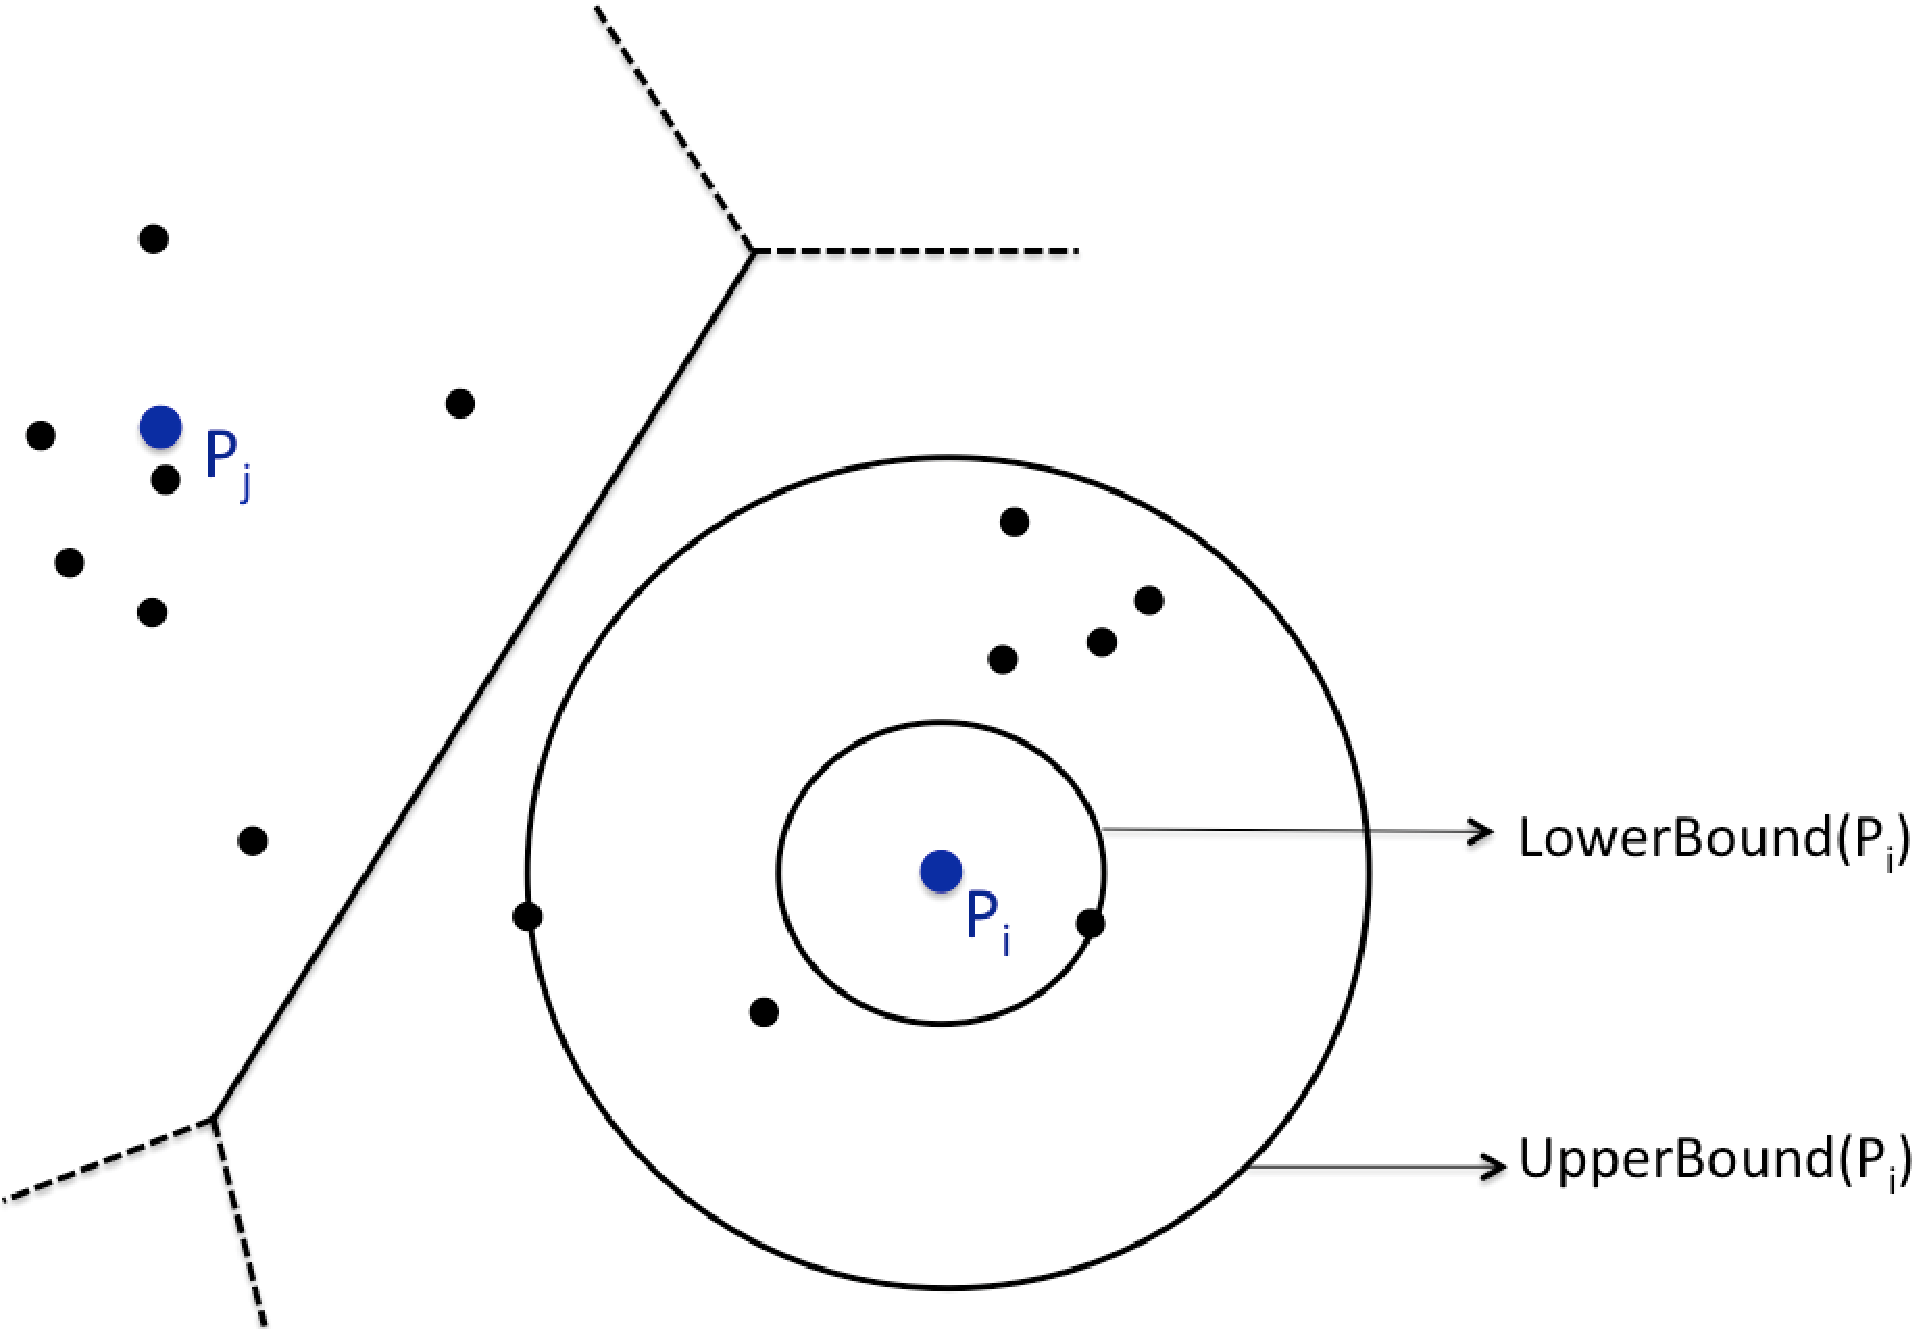
\includegraphics{res/voronoi-partition.pdf}}
\caption{Voronoi based partitioning for pivots $P_i$ and $P_j$ \label{voronoi_partition_figure}}
\end{figure}

Paper \cite{Lu:2012:EPK:2336664.2336674} gives a method to partition the dataset $R$ and $S$ using Voronoi diagram. 
After having identified the pivots in $R$ (as seen in the preprocessing section - \ref{data_preprocessing}), they compute the distance between every point and 
the pivots, and put the considered point into the cell of the closest pivot. This will  naturally give a partitioning of data. Afterwards, they also 
calculate, for each cell of $R$,
the upper (resp. lower) bound of the partition which corresponds to the sphere determined by the furthest (resp. closest) point (in $S$) from the pivot in 
the cell of $R$. Such bounds enable to quickly find the correct partition $S_j$ for a given partition $R_i$.
This data partitioning principle is shown in Figure~\ref{voronoi_partition_figure} where two pivots $P_i$ and $P_j$ have been chosen from the dataset.
%of the nearest neighbors in $S$ for each partition of $R$ to find out the corresponding partition of $S$ \TODO{rewrite}.

The main problem of this method is that it requires computing the distance of all elements to the pivots. Also, the distribution of the input data might 
not be known in advance. Hence, the pivots will have to be recomputed if the data changes, which limits dynamicity. Also, there is no 
guarantee that all cells will have an equal number of elements because of potential data skew. This can have a negative impact on the overall performance
because of load balancing issues.  

\subsubsection{Size Based Partitioning} 

Another type of partitioning method aims at dividing the data into some equal size partitions while preserving their locality 
information. \cite{Zhang:2012:EPK:2247596.2247602} proposes a partitioning strategy based on $z$-value described in the 
previous section. 
%They first compute the $z$-value of every points in $R$. 
In 
order to make every partition of $R$ have a similar number of objects, a sampling is first performed. They claim that the $n$ quantiles 
($n$ is equal to the number of partitions) of the sampling data is an unbiased estimation of the boundary point of each partition, with a
standard deviation $\leq$ $\epsilon\left|R\right|$ $\left( \epsilon > 0\right)$.
After having partitioned $R$ this way, the same sampling strategy is applied to $S$. For each of the boundary points 
of all $R_i$, the corresponding $k^{th}$ nearest neighbor is identified in $S$. These points are then used as boundary points of the corresponding $S_i$.
As a consequence, the partitions of $S$ are overlapping such that for any given point in $R$, all the $k$ nearest neighbors can always be found in a 
single partition of $S$. An example of $z$-value based partition is  given in Figure~\ref{projection_partition_figure}.
\begin{figure}[t]
\centering
\scalebox{0.20}{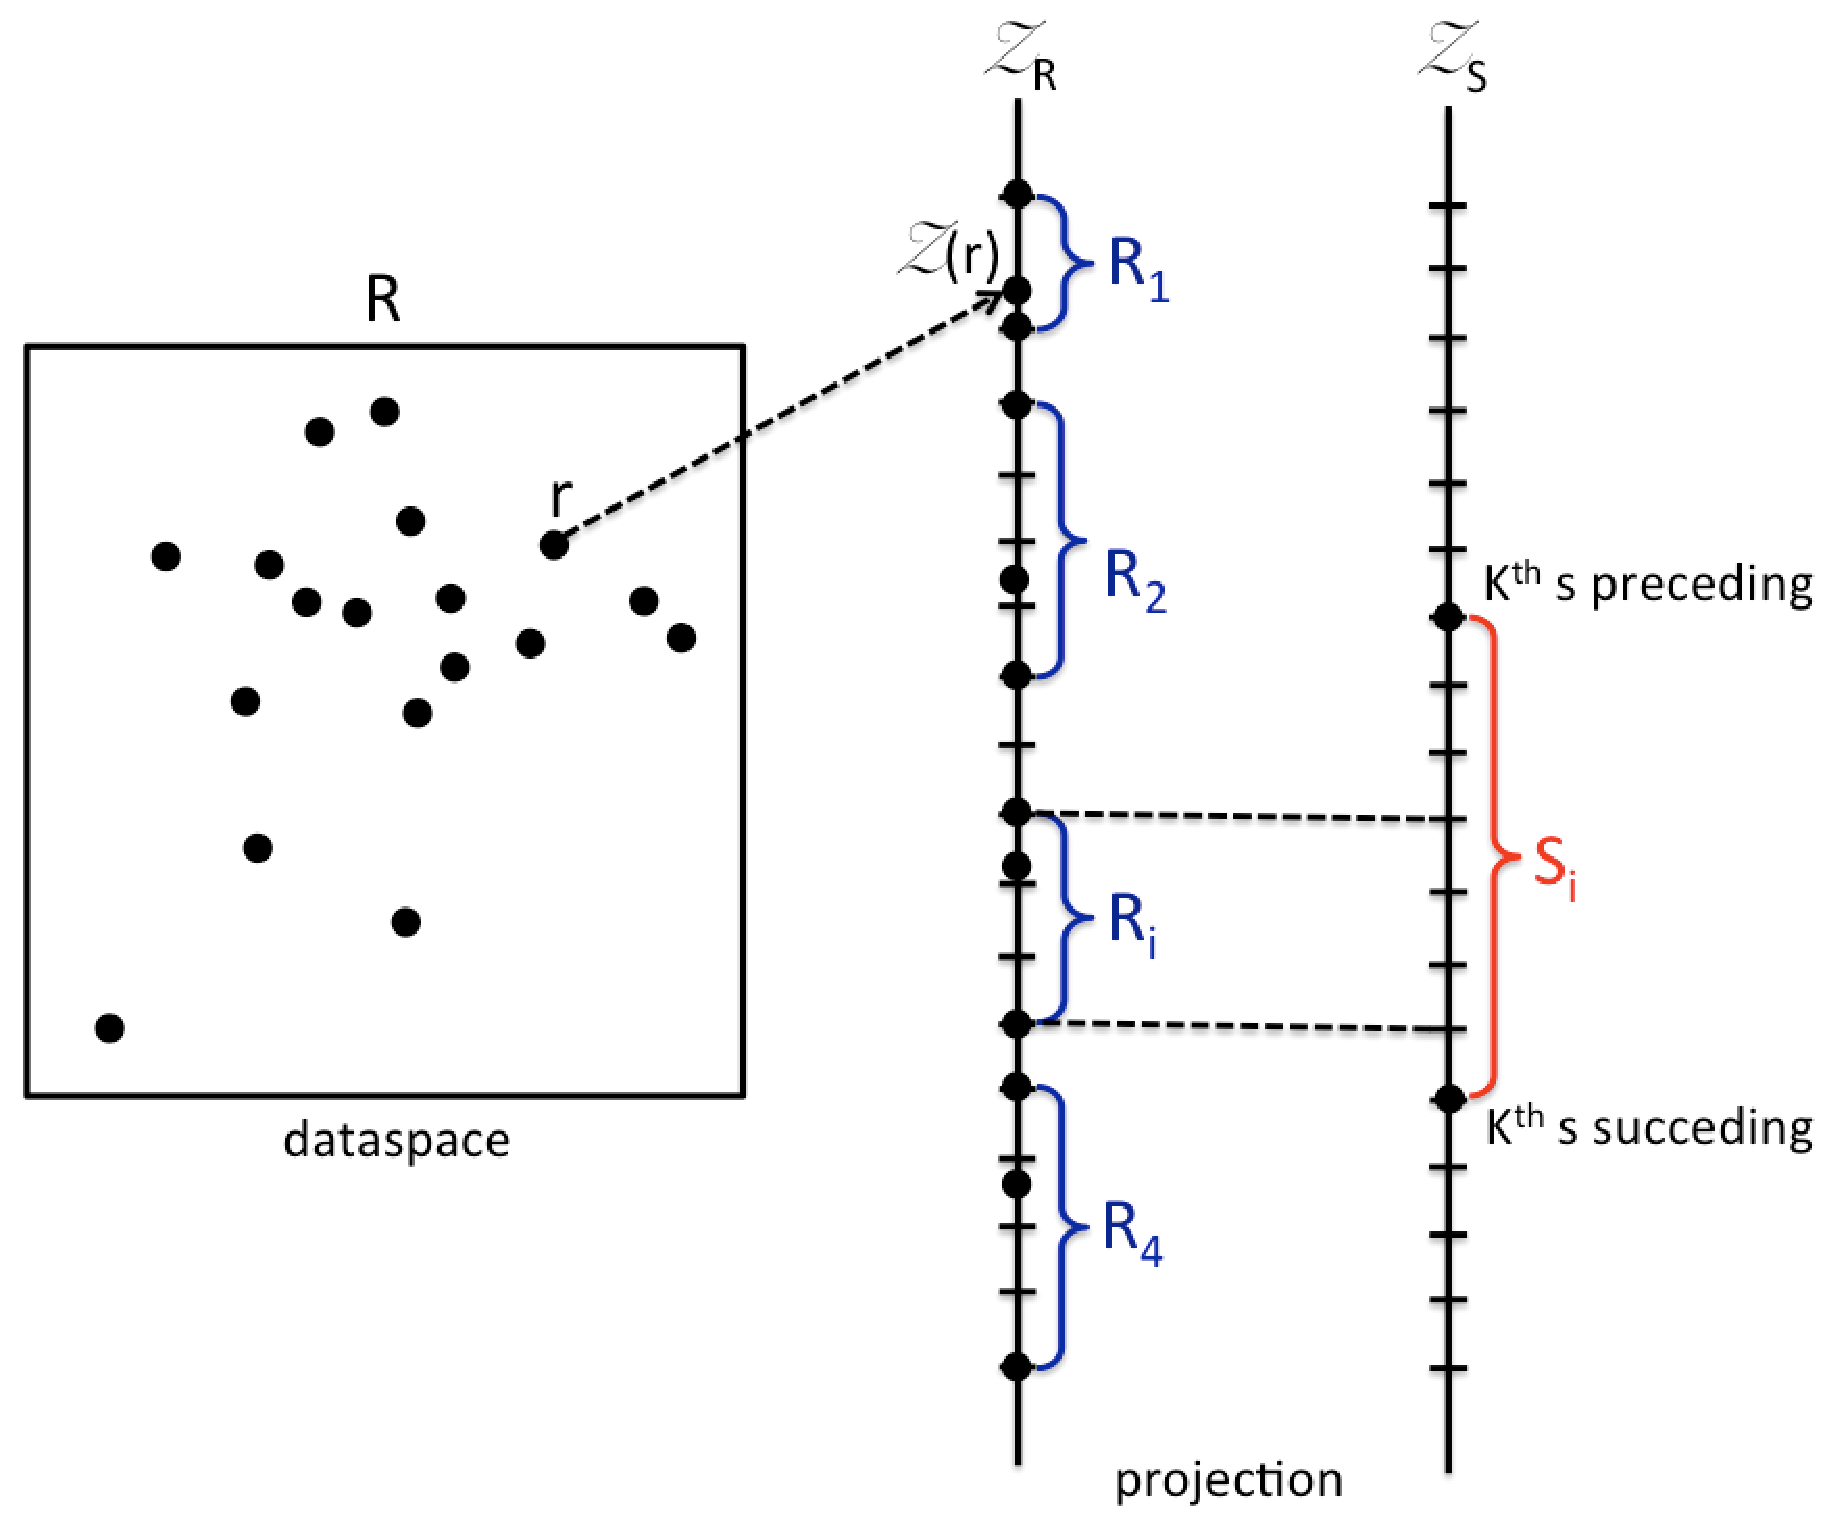
\includegraphics{res/projection-partition.pdf}}
\caption{$z$-value based partitioning \label{projection_partition_figure}}
\end{figure}
This method is likely to produce a substantially equivalent number of objects in each partition. 

Another similar size based partitioning method can be applied for datasets that are preprocessed with \emph{Locality Sensitive Hashing}, as illustrated in 
Figure~\ref{lsh_partition_figure}. With this method, the elements of $R$ that are projected to $LSH(R)$, are divided into 
quasi-equal size partitions using a sampling technique. The same technique can be applied to $S$ and $LSH(S)$. 



%To conclude this section, two kinds of partitioning method can be applied. The first kind, that we have called distance based partitioning, enables a 
%straight-forward partitioning of the raw data around pivots. However, this methods does not guarantee that all the $k$ nearest neighbors 
%will be found in a single partition. The number of partitions of $S$ needed to satisfy query points in a given partition of $R$ is dependent on the number 
%of partitions and the number of elements in each of them \TODO{check}. On the other hand, the second kind of partitioning method, called size based 
%partitioning, ensures to find all the $k$ 
%nearest neighbors in a constant number of partitions, for example, three partitions at maximum in \cite{Zhang:2012:EPK:2247596.2247602} (the one 
%considered and the ones directly to the left and to the right \TODO{not clear, the text above claim they need a single partition}). 
%To conclude this section, two kinds of partitioning methods can be applied for separating data while preserving their locality relationship. 
The strategy of partitioning will impact directly the number of tasks and the amount of computation. Distance based methods aim at dividing the close objects together by pre-selecting some pivots. Size based methods want to separate objects into equal size zones in which the points are ordered.
Regarding the implementation, \cite{Lu:2012:EPK:2336664.2336674} uses a MapReduce job to 
perform the partitioning. In \cite{Zhang:2012:EPK:
2247596.2247602}, both data preprocessing and data partitioning are completed in one MapReduce job.

\begin{figure}[t]
\centering
\scalebox{0.25}{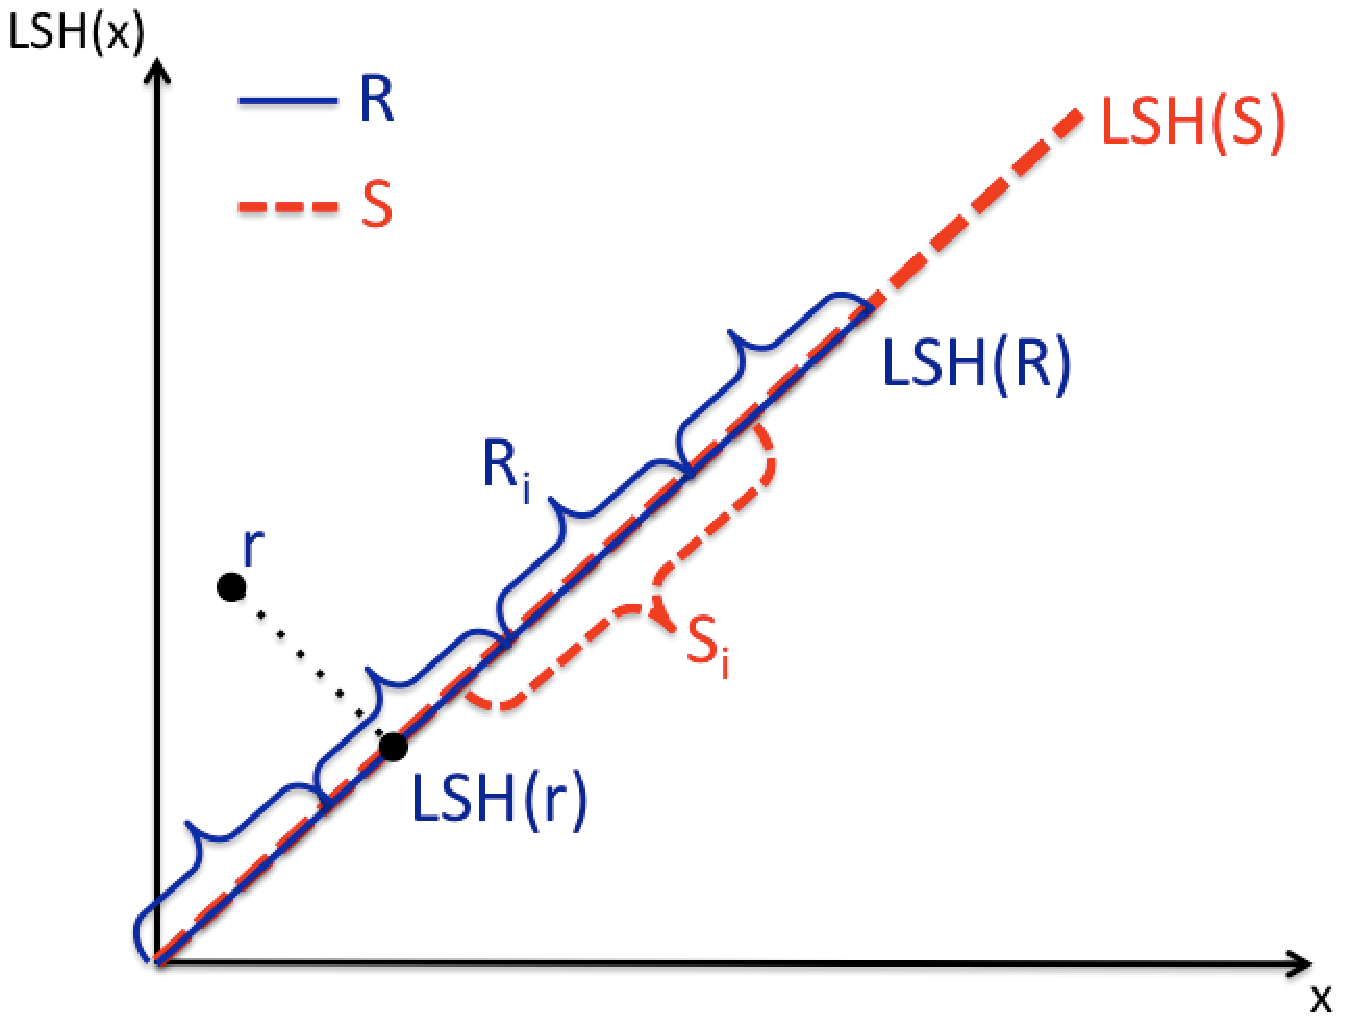
\includegraphics{res/lsh-partition.pdf}}
\caption{LSH based partitioning \label{lsh_partition_figure}}
\end{figure}
%LSH is an approximate approach and }. 
%Although it's more probable for the related objects to have the same hash value than the distance ones, normally one hash function can not guarantee
%the accuracy. We often need a group of hash functions to generate multiple hash tables to avoid the conflict probability of close objects.  



\subsection{Data Partitioning and Selection}
\label{partitioning}

MapReduce is a shared-nothing platform, so in order to process data on MapReduce, we need to divide the dataset into independent pieces, 
called partitions. When computing a kNN, we need to divide $R$ and $S$ respectively.
As in any MapReduce computation, the data partition strategy will strongly impact CPU, network communication and disk usages, which in turn will impact the overall processing time \cite{DBLP:conf/hpcc/SongMHMYL13}. Besides, a good partition strategy could help to reduce the number of data replications, thereby reducing the number of distances needed to be calculated and sorted.

However, not all the algorithms apply a special data partition strategy. For example, H-BNLJ simply divides $R$ into rows and $S$ into lines, making each subset of $R$ meeting with every subset of $S$. This ensures the distance between each object $r_i$ in $R$ and each object $s_j$ in $S$ will be calculated. This way of dividing datasets causes a lot of data replications. For example, in H-BNLJ, each piece of data is duplicated $n$ times (n is the number of subsets of $R$ and $S$), resulting in a total of $n^2$ tasks to calculate pairwise distances. This method wastes a lot of hardware resources, and ultimately leads a low  efficiency.

The key to improve the performance is to preserve spatial locality of objects when decomposing data for tasks \cite{Zhou:1998:DPP:594718.594759}. This means making a coarse clustering in order to produce a reduced set of neighbors that are candidates for the final result. Intuitively, the goal is to have a partitioning of data such that an element in a partition of $R$ will have its nearest neighbors in only one partition of $S$. 
Two partitioning strategies that enable to separate the datasets into independent partitions, while preserving locality 
information, have 
been proposed. They are described in the two next sections. 

\subsubsection{Distance Based Partitioning Strategy}
The distance based partitioning strategy we study in this paper is based on Voronoi diagram, a method to divide the space into disjoint cells. We can find other distance-based partitioning methods in the litterature, such as in~\cite{Ji:2012:IGK:2408853.2408998}, but we chose Voronoi diagram to represent distance-based partitioning method because it it can apply to data in any dimension. 
The main property of Voronoi diagram 
is that every point in a cell is
closer to the pivot of this cell than to any other pivot. More formally, the 
definition of a Voronoi cell is as follow:
\begin{myDef}
Given a set of disjoint pivots: \\ P = $\left\{ p_1, p_2, ..., p_i, ..., p_n \right\}$, the Voronoi Cell of $p_i$ $\left(0 < 
i \leq n \right)$ is: $
\forall$ i $\neq$ j, $VC\left(p_i\right) = \left\{p \| d\left(p, p_i\right) \leq d\left(p, p_j\right) \right\}$. 
\end{myDef}


Paper \cite{Lu:2012:EPK:2336664.2336674} gives a method to partition  datasets $R$ and $S$ using Voronoi diagram. 
The partitioning principles are illustrated in Figure~\ref{fig:voronoi_partition_figure}. 
\begin{figure}[h]
\centering
\scalebox{0.33}{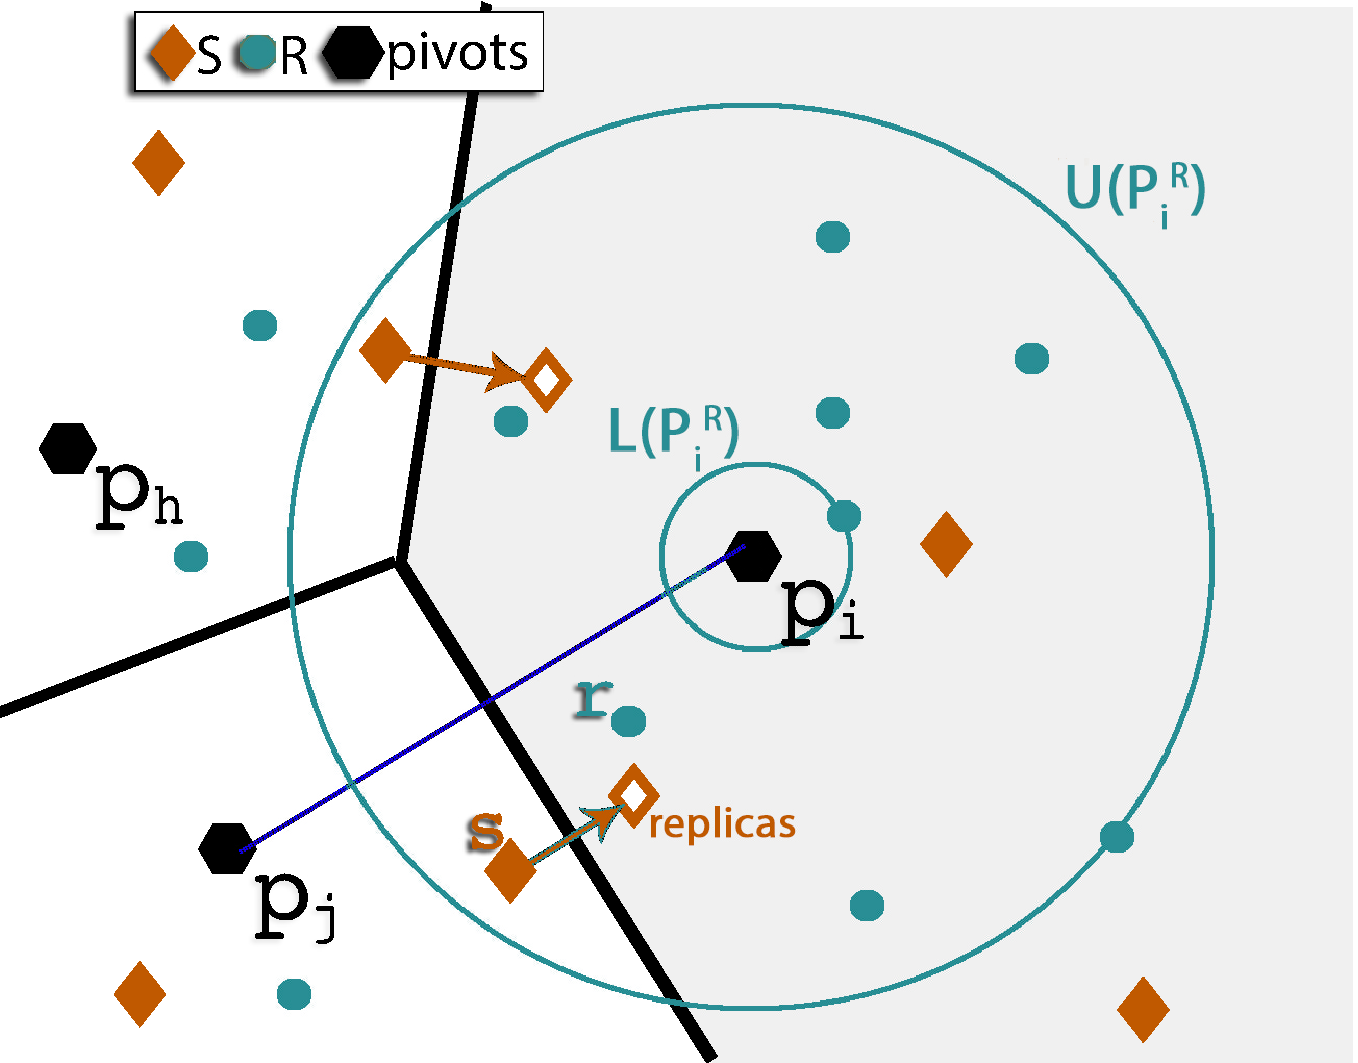
\includegraphics[width=\textwidth]{voronoi-partition.pdf} }
                \caption{Voronoi : cells partitioning and replication for cell $P_i$%based partitioning %for pivots $P_i$ and $P_j$
                }
                \label{fig:voronoi_partition_figure}         
\end{figure}%
After having identified the pivots $p_i$ in $R$ (c.f. Section~ \ref{data_preprocessing}), the distances between 
elements of each dataset and the pivots are computed. The elements are then put in the cell of the closest 
pivot, giving a partitioning of $R$ (resp. $S$) into $P_i^R$ (resp. $P_i^S$). For each cell, the upper bound 
$U(P^{R}_{i})$ (resp. the lower bound $L(P^{R}_{i})$) is computed as a sphere determined by the furthest (resp. 
nearest) point in $P_i^R$ from the pivot $p_i$.  The boundaries and other statistics are used to find 
candidate data from S in the neighboring cells. These data are then replicated in cell $P_i^S$. For example, in 
Figure~\ref{fig:voronoi_partition_figure}, the element $s$ of $P^{S}_{j}$ falls inside $U(P^{R}_{i})$ and is thus 
copied to $S_i$ as a potential candidate for the kNN of $r$.% \TODO{Check paper}. 



The main issue with this method is that it requires computing the distance from all elements to the pivots. Also, the distribution of the input data might 
not be known in advance. Hence, pivots have to be recomputed if data change.
 More importantly, there is no 
guarantee that all cells have an equal number of elements because of potential data skew. This can have a negative impact on the overall performance
because of load balancing issues. To alleviate this issue, the authors propose two grouping strategies, which will be discussed in 
Section~\ref{sec:load_balance}.

\subsubsection{Size Based Partitioning Strategy} 

Another type of partitioning strategy aims at dividing data into equal size partitions. Paper \cite{Zhang:2012:EPK:2247596.2247602} proposes a partitioning strategy based on $z$-value described in the 
previous section. 

In order to have a similar number of elements in all $n$ partitions, the authors first sample the dataset and compute the $n$ quantiles. These quantiles are an  unbiased estimation of the bounds for each partition. Figure~\ref{projection_partition_figure} shows an example for this method. In this example data are only shifted once. Then, data are projected using $z$-value method, and the interpolating ``Z" in the figure indicates the neighborhood after projection. Data is projected into a one dimension space, represented by 
$Z_{i}^{R}$ and $Z_{i}^{S}$ in the figure. $Z_{i}^{R}$ is divided into partitions using the sampling estimation explained above. For a given partition $R_i$, its corresponding $S_i$ is defined in $Z_{i}^{S}$ by copying the nearest $k$ preceding and the nearest $k$ succeeding points to the boundaries of $S_i$.
In  Figure~\ref{projection_partition_figure}, four points of $S_i$ are copied in partition 2, because they are considered as candidates for the query points in $R_i^2$.

 
\begin{figure}[h]
\centering
\scalebox{0.33}{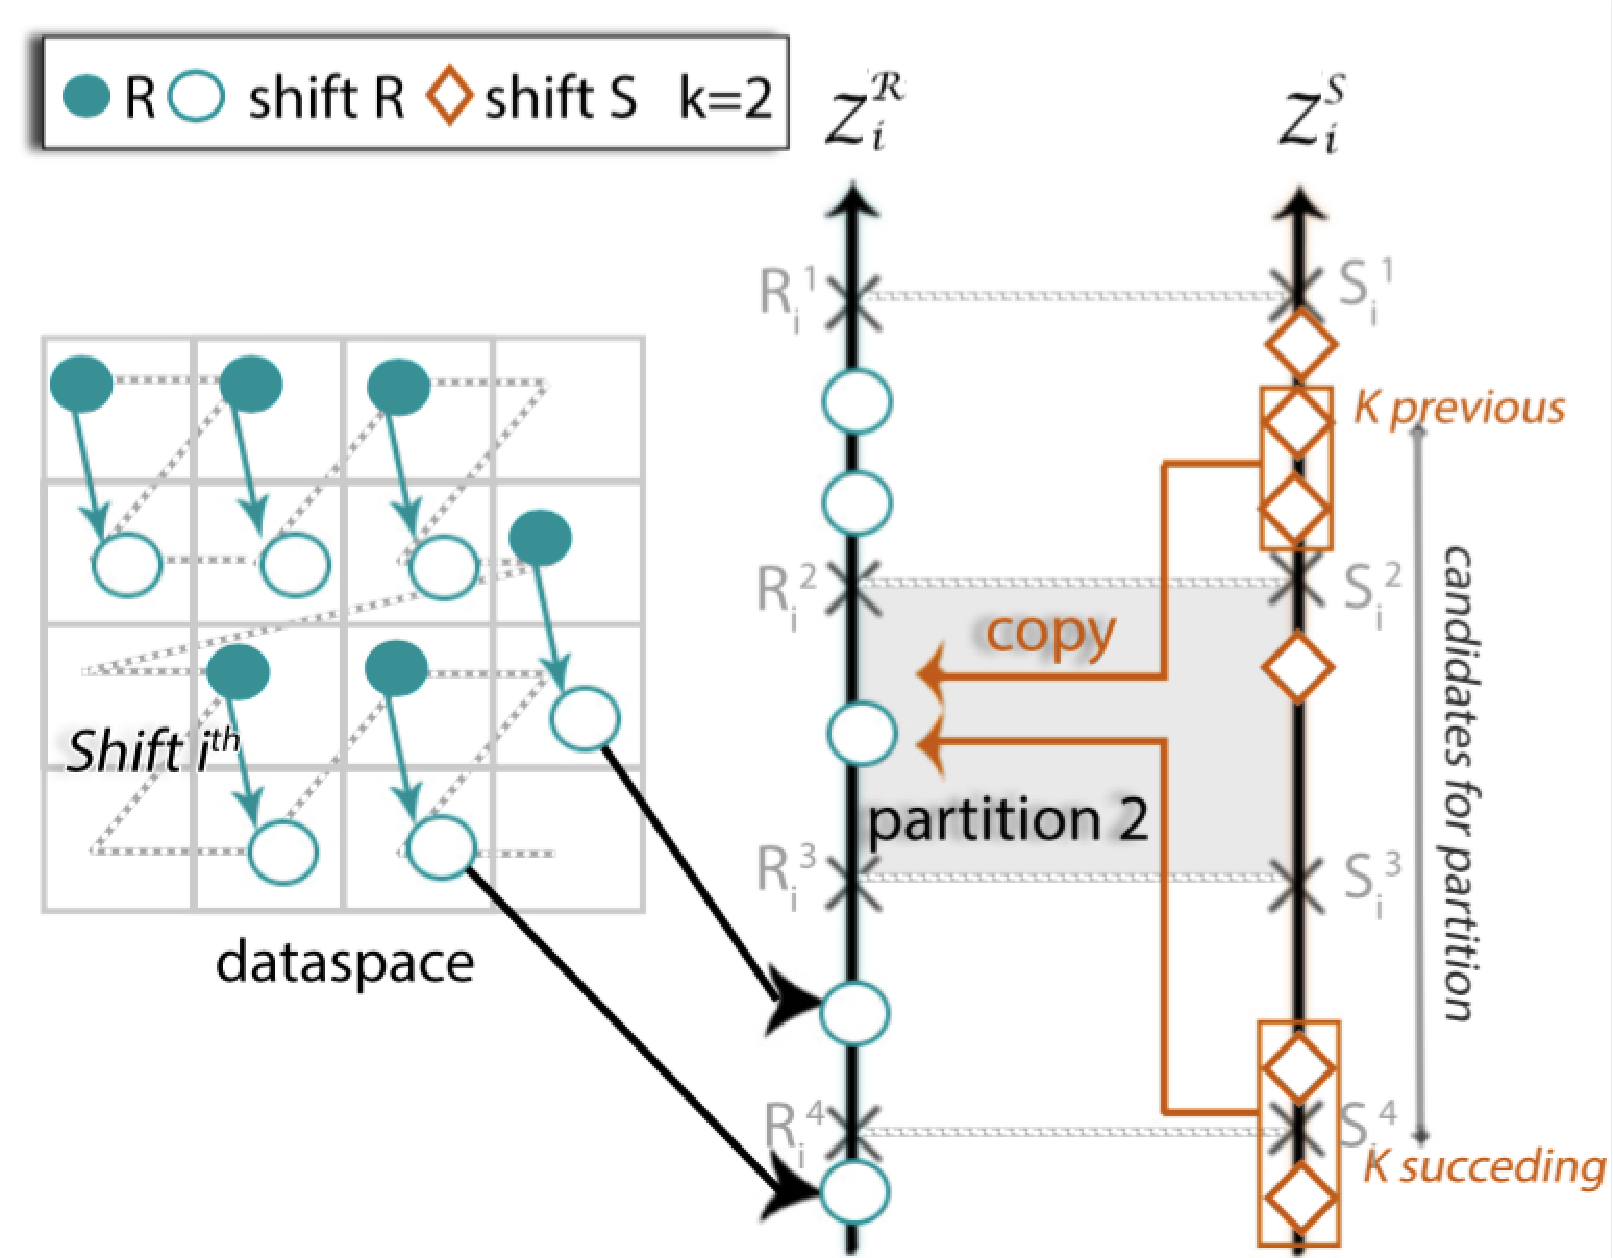
\includegraphics{projection-partition.pdf}}
\caption{$z$-value : partition \label{projection_partition_figure}}
\end{figure}


This method is likely to produce a substantially equivalent number of objects in each partition, thus naturally 
achieving load balancing. However, the quality of the result depends solely on the quality of the $z$-curve, which 
might be an issue for high dimension data. 


 
Another similar size based partitioning method uses Locality Sensitive Hashing to first project data into low dimension 
space as illustrated in Figure~\ref{lsh_partition_figure}. In this example, data is hashed twice using two hash 
families $a1$ and $a2$. Each hashed data is then projected in the corresponding bucket. The principle of this method is 
to result in collisions for data that is spatially close. So the data initially close in the high dimension space is 
hashed to the same bucket with a high probability, provided that the bucket size (parameter $W$ in LSH) is large enough 
to receive at least one copy of close data. 

 
The strategy of partitioning directly impacts on the number of tasks and the amount of computation. Distance based 
methods aim at dividing the space into cells that are driven by distance rules. Size based methods create equal size 
zones in which the points are ordered.
Regarding the implementation, \cite{Lu:2012:EPK:2336664.2336674} uses a MapReduce job to 
perform the partitioning. In \cite{Zhang:2012:EPK:2247596.2247602}, both data preprocessing and data partitioning are completed in a single MapReduce job.

\begin{figure}[h]
\centering
\scalebox{0.33}{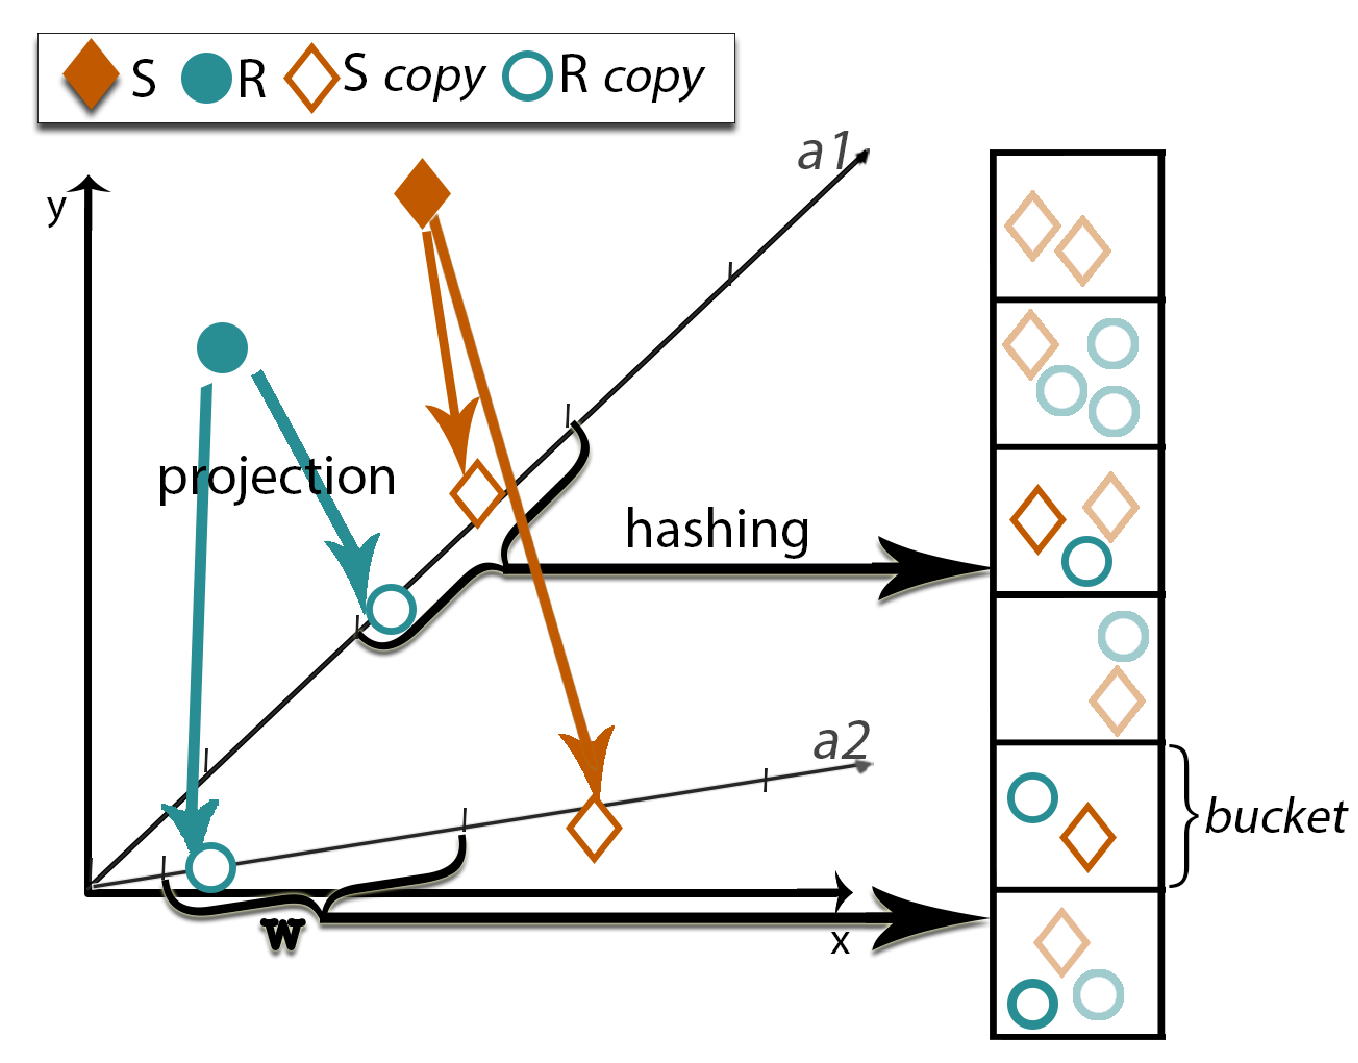
\includegraphics{lsh-partition.pdf}}
\caption{LSH : bucket \label{lsh_partition_figure}}
\end{figure} 

%\subsection{Computation} 

%\TODO{--CHECK--}
The general idea to compute a kNN, is to (i) calculate the distance between $r_i$ and $s_j$ for all $i$ and all 
$j$, and (ii) sort these distances in ascending order to 
find out the first $k$ results. In MapReduce, the idea is the same except that what is given to a task must be independent in order to ensure correctness without duplicating the whole dataset. The number of MapReduce jobs used for computing and sorting has
an impact on the global performance, given the complexity of the computation performed by each task and the amount of data to exchange between them. 
The preprocessing and partitioning steps can also affect the number of tasks that are further needed by each MapReduce job. 
%Also, the pre-processing and the partitioning of the data can also be performed with MapReduce. Hence, 
%depending on the chosen workflow, many different jobs are involved. 
In this section, we review the 
different strategies used to compute and sort distances efficiently using MapReduce. These different strategies can be divided into two categories: the ones 
using one round of MapReduce job and the ones using two rounds of MapReduce jobs. Then, those categories can be divided into two subcategories: the ones that do 
not preprocess and partition data before computation and the ones that implement the preprocessing and partitioning steps. We detail all these 
strategies in the following.

\subsubsection{One Round of MapReduce Job}

\textbf{Without preprocessing and partitioning.} 
The basic idea (H-BkNNJ) to compute a kNN with MapReduce is to have every Map task process a 
pair of $R_i$ and $S_j$, and perform a block nested loop on them to calculate the distance between $r_i \in 
R_i$ and $s_j \in S_j$,  $\forall$ $i$ and $j$. Note that, without any smart partitioning strategy, every possible blocks of one partition $R_i$ from $R$ and $S_j$ from $S$ should be calculated, leading to $n^2$ tasks totally where n is the number of partitions of $R$ and $S$.
%$S_j$ must represent the whole dataset $S$ to produce a correct output.
The output of the Map task is in the form of $\left(id(r_i), list
\left( id(s_{j}), d\left(r_i, s_j\right)\right)\right)$. The identifier of $r_i$, named $id(r_i)$, is used as a key and the 
associated value is a list containing the identifier of $s_j$ and the computed distance between $r_i$ and $s_j$. A reduce task then 
processes all computed distances for a given $r_i$, and sorts them in ascending order to 
output the top $k$ results. 
%This basic idea is explained in more details in \cite{Zhang:2012:EPK:2247596.2247602}.
%tasks will take the same partitions from the output of the Map tasks, merge all the results of the same key 
%together and sort $d\left(r_i, s_j\right)$ 
%in a descending order, and emit the top $k$ results. 
%Figure~\ref{knn_mapreduce} shows the basics of this process.
%\begin{figure}[t]
%\center
%\scalebox{0.3}{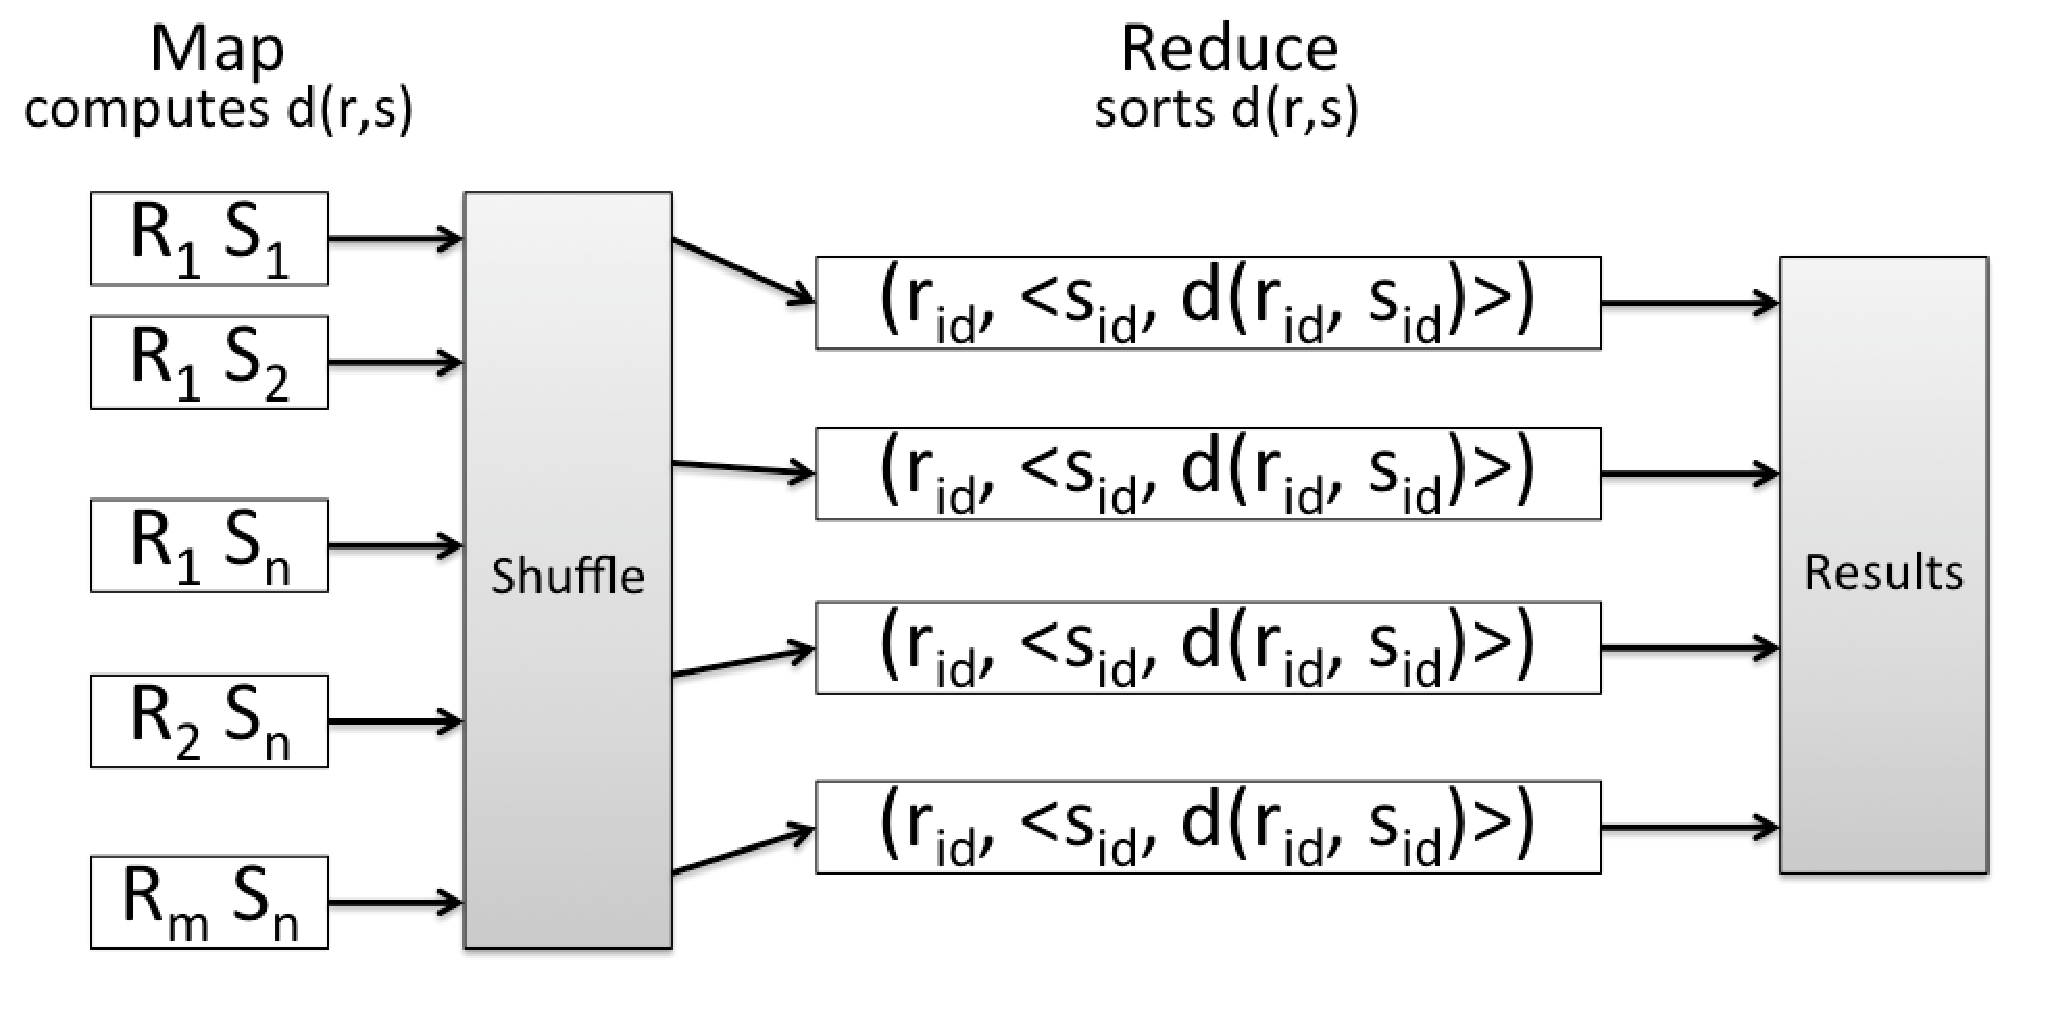
\includegraphics{res/knn-mapreduce.pdf}}
%\caption{Basic idea for processing kNN join in MapReduce \label{knn_mapreduce}}
%\end{figure}
\begin{figure*}[t]
\center
\scalebox{0.35}{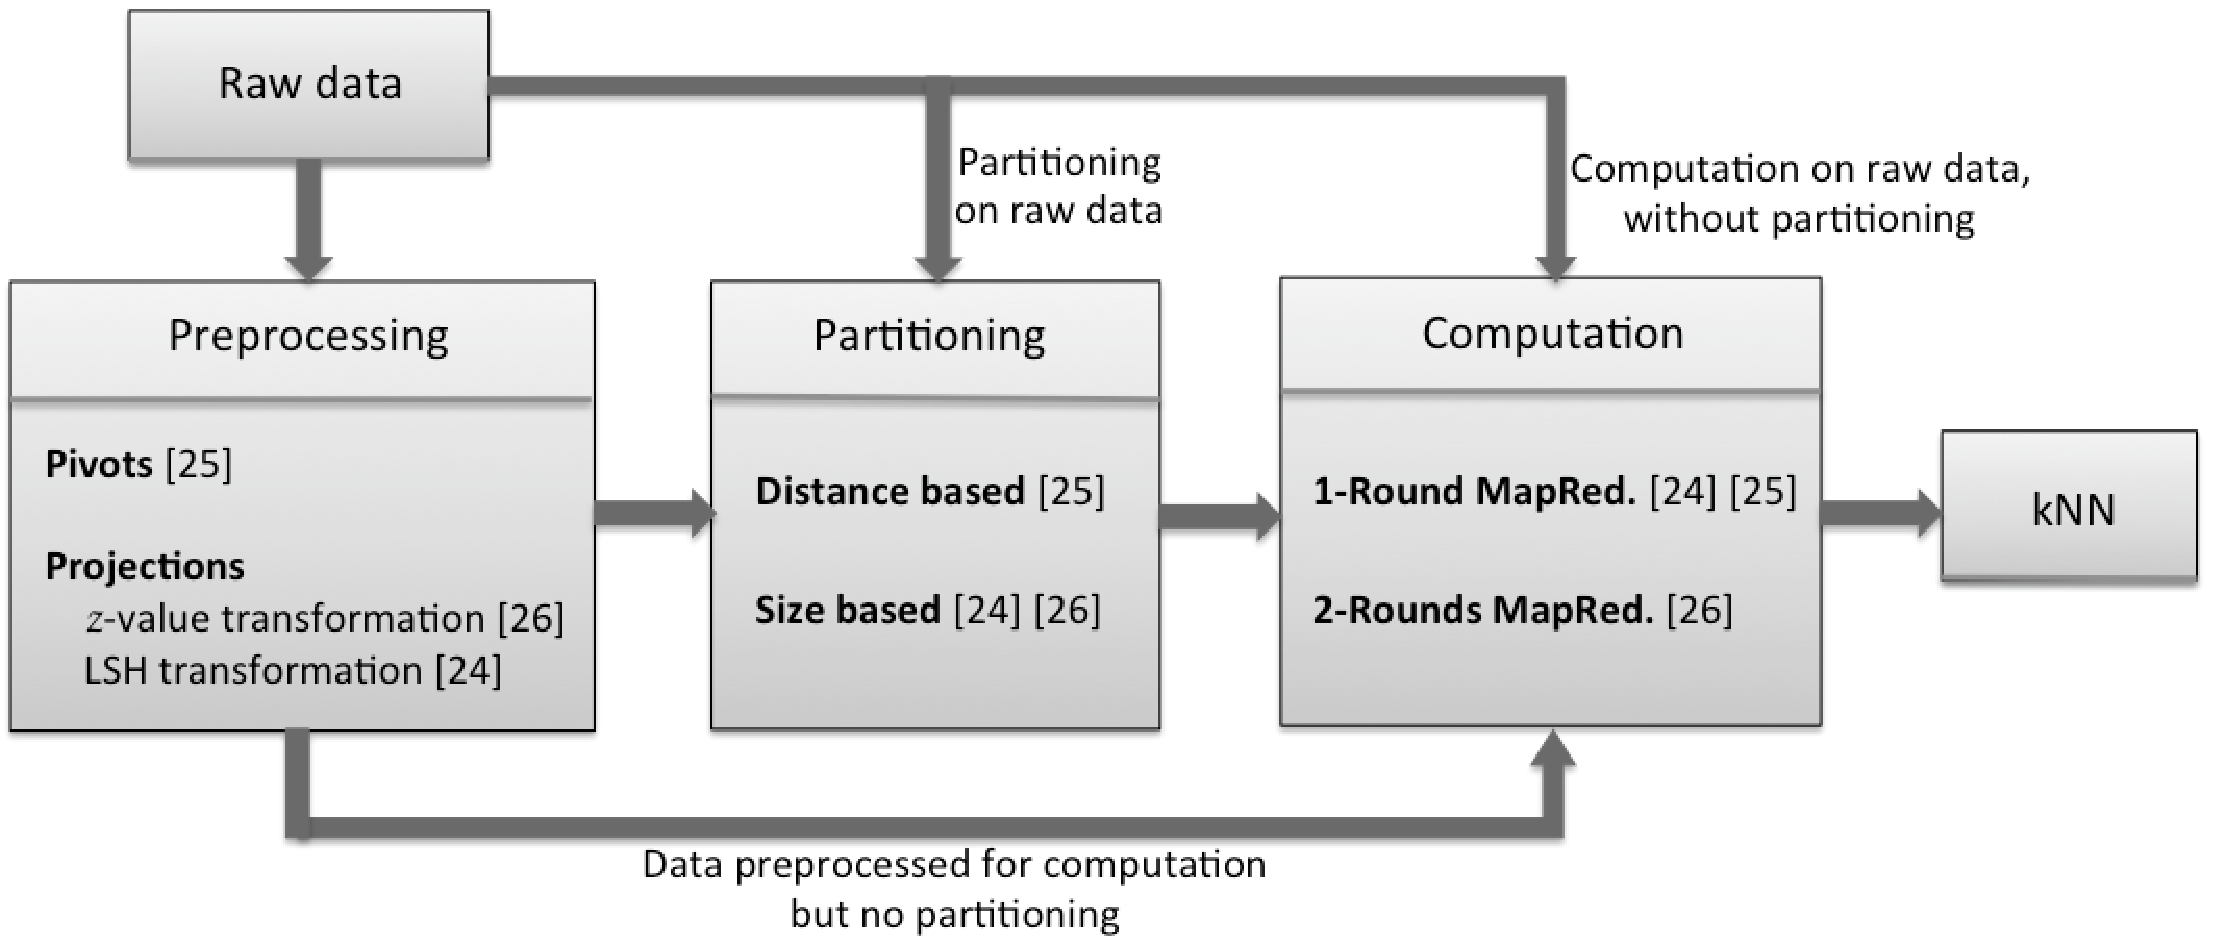
\includegraphics{res/workflow.pdf}}
\caption{Usual workflow of a kNN computation using MapReduce \label{workflow}}
\end{figure*}


\textbf{With preprocessing and partitioning.} To reduce the number of tasks used to calculate the distances, in other words, to reduce the number of pairs formed by $R_i$ and $S_j$, PGBJ \cite{Lu:2012:EPK:2336664.2336674} uses a preprocessing and distance based partitioning strategy, which ensures that each partition $R_i$ has only one corresponding partition $S_i$ needed to be searched, which reduces the number of tasks to $n$. %In this work, 
%they pre-select similar objects (close points) in $R$ and form a partition with them using distance based partitioning 
%\TODO{not already explained in previous section? --CHECK--}
%, and they subsequently find the 
%corresponding partition in $S$. 
Once the blocks of $R_i$ and $S_i$ identified, they perform the same calculation as in the H-BkNNJ technique. Because of 
their data organization, they are able to reduce the number of tasks, greatly improving the performance.

In RankReduce \cite{Stupar10rankreduce-}\footnote{Although RankReduce only compute kNN for a single query, it is 
easy to extend it to a full kNN join}, the authors first preprocess and partition data into buckets using 
LSH. Their Map function computes the distance of all points in the partition, and then sorts the local distances to output the local 
 $k$ nearest neighbors for each point in the partition, together with their distance in form of $\left(id(r_i), list
\left( id(s_{j}), d\left(r_i, s_j\right)\right)\right)$.
 %$\left(query, \left(neighbor, distance\right)\right)$. 
 %\TODO{why don't we have the same notation than before with ri, d() ...}
These key-value pairs are then pulled by Reducers where they are sorted and issued as final results.

Overall, the main limitation of these approaches is that the number of values to be sorted in the reduce phase
can be extremely large, up to $\left|S\right|$, if the
pre-processing and partitioning have not significantly reduced the set of candidate points.
%when the filtering on the reference points is too coarse. \TODO{reference points? can we say: if the
%pre-processing and partitioning have not significantly reduced the set of candidates}.
%\TODO{I don't like partitioning here, another word like filtering? -- ?? --}. 
This greatly limits the applicability of such approach. 


\subsubsection{Two Rounds of MapReduce Jobs}
\textbf{Without preprocessing and partitioning.} 
To overcome the previously described limitation, multiple successive MapReduce jobs are required. The idea is to have the first job output
the top $k$ for each pair ($R_i$, $S_j$). Then, the second job is used to merge all the top $k$ values for a 
given $r_i$ and to perform the merging and sorting of all local top $k$ values (instead of all values), producing the final global top $k$. Such approach is used in H-BNLJ 
\cite{Zhang:2012:EPK:2247596.2247602} and greatly improves sorting time. %And the authors also indicate that we can index the local blocks of S by R-Tree and improve H-BNLJ to H-BRJ.\TODO{is this related to this section?}

%H-BkNNJ method only uses one MapReduce job, but we need to sort $\left|S\right|$ numbers of $d\left(r_i, s_j\right)$ for every object $r_i$. The sort
%algorithm in MapReduce is Quick Sort and Merge Sort by default, their complexity is $\left|S\right| \times Log \left|S\right|$. When $\left|S\right|$ is 
%large, this process is very time consuming. So, paper \cite{Zhang:2012:EPK:2247596.2247602} gives an improvement H-BNLJ. H-BNLJ uses two MapReduce jobs 
%to achieve the same goal. Mapper 1 will get a piece of $R_i$ and $S_j$, Reducer 1 will calculate the distance between $\forall$ $r_i \in R_i$ and $s_j 
%\in S_j$, Mapper 2 sort the results of Reducer 1 and emit the local top $k$ results, Reducer 2 pull the local result of the same key, merge and sort them 
%then give the global top $k$ results. The authors also point out that we can use some index structures like R-Tree to index the local $S$ blocks in order 
%to speed up finding the nearest neighbors.


\textbf{With preprocessing and partitioning.} 
A last possibility is based on the z-value preprocessing.
%the two previous methods: one job for pre-processing and partitioning, one for 
%computing the distances, and a lost one for filtering and sorting the results. 
In H-zkNNJ \cite{Zhang:2012:EPK:2247596.2247602} the authors propose to generate several shifted copies of $R$ and $S$ (to improve the 
accuracy), and to determine the bounds of the partitions of $R_i$ and the 
corresponding $S_i$ in a pre-processing MapReduce job. So here, the preprocessing and partitioning step is completely integrated in MapReduce. Then, the first MapReduce round of computation takes the partitions $R_i$ and $S_i$ previously determined, and computes the candidate neighbor set, named 
$C_i\left(r\right)$,  for $\forall r_i \in R_i$, which contains $k$ local nearest objects immediately before $r_i$ and $k$ objects after $r_i$ ($2k$ objects totally). %\TODO{not clear. Notation seems inconsistent, why r and not r\_i?}
The second MapReduce round decides the exact result $\forall r_i \in R$ from the candidate neighbor set $kNN\left(r, C_i\left(r\right)\right)$.
%\TODO{how? what does the job do in practice?}
%\TODO{don't like kNN(r,...) here, can it be simpler?}
So in total, three MapReduce jobs are launched, and among them, two are actually devoted to the kNN computation. As the number of points that are in the candidate neighbor set is small, thanks to the drastic partitioning (itself due to a drastic preprocessing), the cost of computation and communication is extremely reduced.

\subsection{Computation} 
The main principle to compute a kNN, is to (i) calculate the distance between $r_i$ and $s_j$ for all $i$, 
$j$, and (ii) sort these distances in ascending order to 
pick the first $k$ results. The number of MapReduce jobs for computing and sorting has
a significant impact on the global performance of the kNN computation, given the complexity of MapReduce task and the amount of data to exchange between them. 
The preprocessing and partitioning steps impact on the number of MapReduce tasks that are further needed for the core computation. 
%Also, the pre-processing and the partitioning of the data can also be performed with MapReduce. Hence, 
%depending on the chosen workflow, many different jobs are involved. 
In this section, we review the 
different strategies used to finally compute and sort distances efficiently using MapReduce. These different strategies can be divided into two categories, depending on the number of jobs they require. Those categories can themselves be divided into two subcategories: the ones that do 
not preprocess and partition data before computation and the ones that implement the preprocessing and partitioning steps. 

\subsubsection{One MapReduce Job}

\noindent \textbf{Without preprocessing and partitioning strategies.} 

\noindent The naive solution (\HBK) only uses one MapReduce job to calculate and sort the distances, and only the Map Phase is done in parallel. The Map tasks will cut datasets into splits, and label each split with its original dataset ($R$ or $S$). The Reduce task then takes one object $r_i$ and one object $s_j$ to form a key-value pair $<r_i, s_j>$, and calculate the distance between them, then for each key $r_i$ sort the distances with every object in $S$, leading the number of distances need to be sorted to $|S|$. Since only the Map phase is in parallel, and only one Reduce task is used for calculating and sorting, when the datasets becomes large, this method will quickly exceed the processing capacity of the computer. Therefore, it is only suitable for small datasets.

\vspace{0.3em}

\noindent \textbf{With preprocessing and partitioning strategies.} 

\noindent \VO~ \cite{Lu:2012:EPK:2336664.2336674} uses a preprocessing step to select the pivot of each partition and a distance based partitioning 
strategy to ensure that each subset $R_i$ only needs one corresponding subset $S_i$ to form a partition where the kNN of all $r_i \in R_i$ can 
be found. Therefore, in the computation step, Map tasks find the corresponding $S_i$ for each $R_i$ according to the information provided by 
the partitioning step. Reduce tasks then perform the kNN join inside each partition of $<R_i, S_i>$.


Overall, the main limitation of these two approaches is that the number of values to be sorted in the Reduce task
can be extremely large, up to $\left|S\right|$, if the
preprocessing and partitioning steps have not significantly reduced the set of searched points.

This aspect can limit the applicability of such approaches in practice. 


\subsubsection{Two Consecutive MapReduce Jobs}
To overcome the previously described limitation, multiple successive MapReduce jobs are required. The idea is to have the first job output the local top $k$ for each pair $(R_i, S_j)$. Then, the second job is used to merge all the top $k$ values for a given $r_i$ and to merge and sort all local top $k$ values (instead of all values) producing the final global top $k$.

\vspace{0.3em}

\noindent \textbf{Without preprocessing and partitioning strategies.} 

\noindent \HBNLJ~ does not have any special preprocessing or partitioning strategy. The Map Phase of the first job distributes $R$ into $n$ rows and $S$ into $n$ columns. The $n^2$ Reduce tasks output the local kNN for each object $r_i$ in the form of $(r_{id}, s_{id}, d(r, s))$.

Since each $r_{id}$ has been replicated $n$ times, the Map Phase of the second MapReduce job will pull every candidate of $r_i$ from the $n$ pieces of $R$, and form $(r_{id}), list(s_{id}, d(r, s))$. Then each Reduce task will sort $list(s_{id}, d(r, s))$ in ascending order of $d(r, s)$ for each $r_i$, and finally, give the top $k$ results.

 Moreover, in order to avoid the scan of the whole dataset of each block, some index structures like R-Tree \cite{Zhang:2012:EPK:2247596.2247602} or Hilbert R-Tree \cite{6967143} can be used to index the local $S$ blocks. 

\vspace{0.3em}

\noindent \textbf{With preprocessing and partitioning strategies.} 


\noindent
In \Z~ \cite{Zhang:2012:EPK:2247596.2247602} the authors propose  to define the bounds of the partitions of $R$ and then to determine from this the 
corresponding $S_i$ in a preprocessing job. So here, the preprocessing and partitioning steps are completely integrated in MapReduce. Then, a 
second MapReduce job takes the partitions $R_i$ and $S_i$ previously determined, and computes for all $r_i$ the candidate neighbor set, which 
represents the points that could be in the final kNN\footnote{Note that the notion of candidate points is different from local top $k$ points.}.
To get this candidate neighbor set, the closest $k$ points are taken from either side of the considered point (the partition is in dimension 1), which leads to exactly 2$k$ candidate points.
The third MapReduce round determines the exact result for each $r_i$ from the candidate neighbor set.
So in total, this solution uses three MapReduce jobs, and among them, the last two are actually devoted to the kNN core 
computation. As the number of points that are in the candidate neighbor set is small (thanks to the drastic 
partitioning, itself due to a drastic preprocessing), the cost of computation and communication is extremely reduced.

In \LSH~ \cite{Stupar10rankreduce-}\footnote{Although RankReduce only computes kNN for a single query, it is 
directly expandable to a full kNN join.}, the authors first preprocess  data to reduce the dimentionality and partition data into buckets 
using LSH. In our implementation, like in \Z,  one MapReduce job is used to calculate the local kNN for each $r_i$, and 
a second one is used to find the global ones.

%\subsection{Summary}
So far, we have studied the different ways to go through a kNN computation from a workflow point of view with three main steps.
The first step focuses on data preprocessing, either for selecting pivots for each partition or for projecting data from high dimension to low dimension.
The second step is in charge of data partitioning and organization in the partitions using distance based method or size based method. The last step of the workflow is to actually compute the kNN in one or two MapReduce jobs. Figure~\ref{workflow} summarizes the 
workflow we have gone through in this section and the techniques that are associated with each step.

%\begin{figure*}[t]
%\center
%\scalebox{0.35}{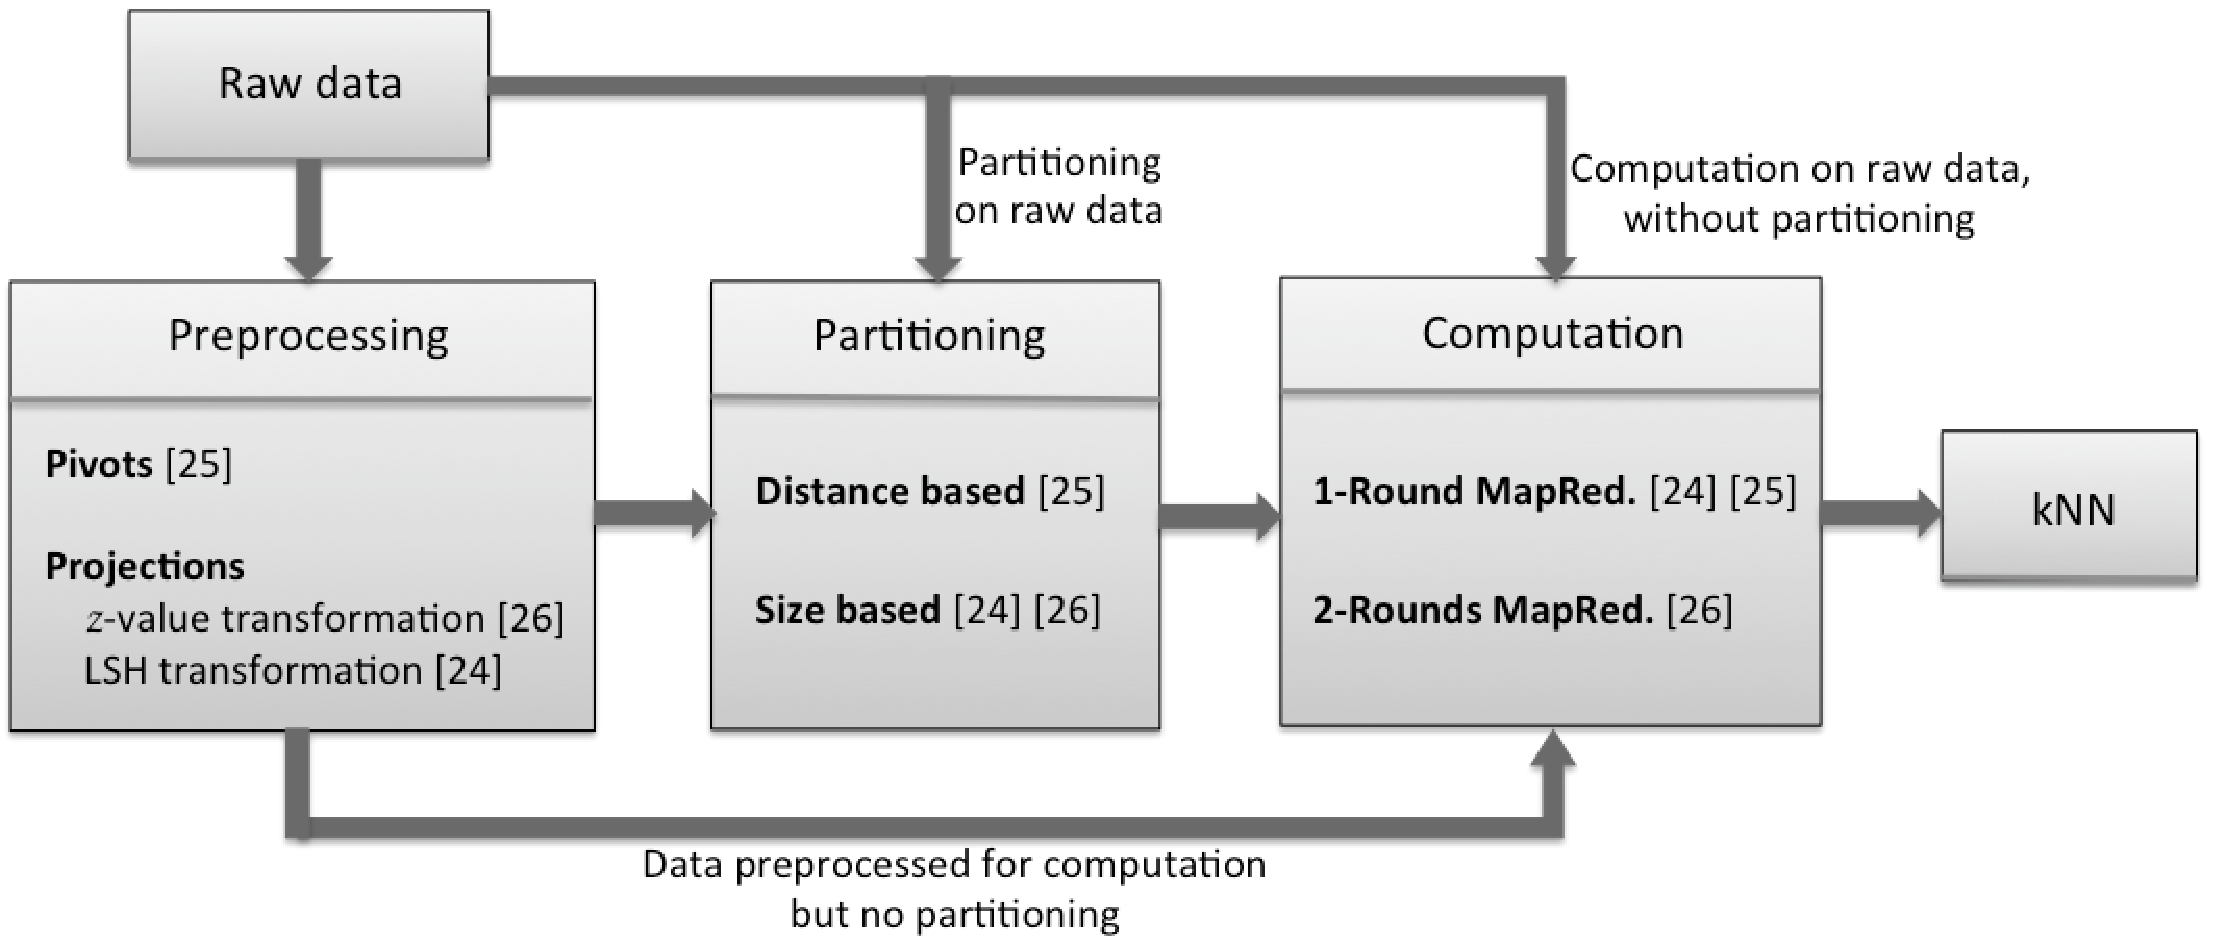
\includegraphics{res/workflow.pdf}}
%\caption{Usual workflow of a kNN computation using MapReduce \label{workflow}}
%\end{figure*}

\subsection{Summary}
So far, we have studied the different ways to go through a kNN computation from a workflow point of view with three main steps.
The first step focuses on data preprocessing, either for selecting dominating points or for projecting data from high dimension to low dimension.
The second step aims at partitioning and organizing data such that the following kNN core computation step is lighten. This last step can use one or two MapReduce jobs depending on the number of distances we want to calculate and sort.
%amount of data that are left from the previous steps. 
\begin{figure*}[htp]
\center
\scalebox{0.35}{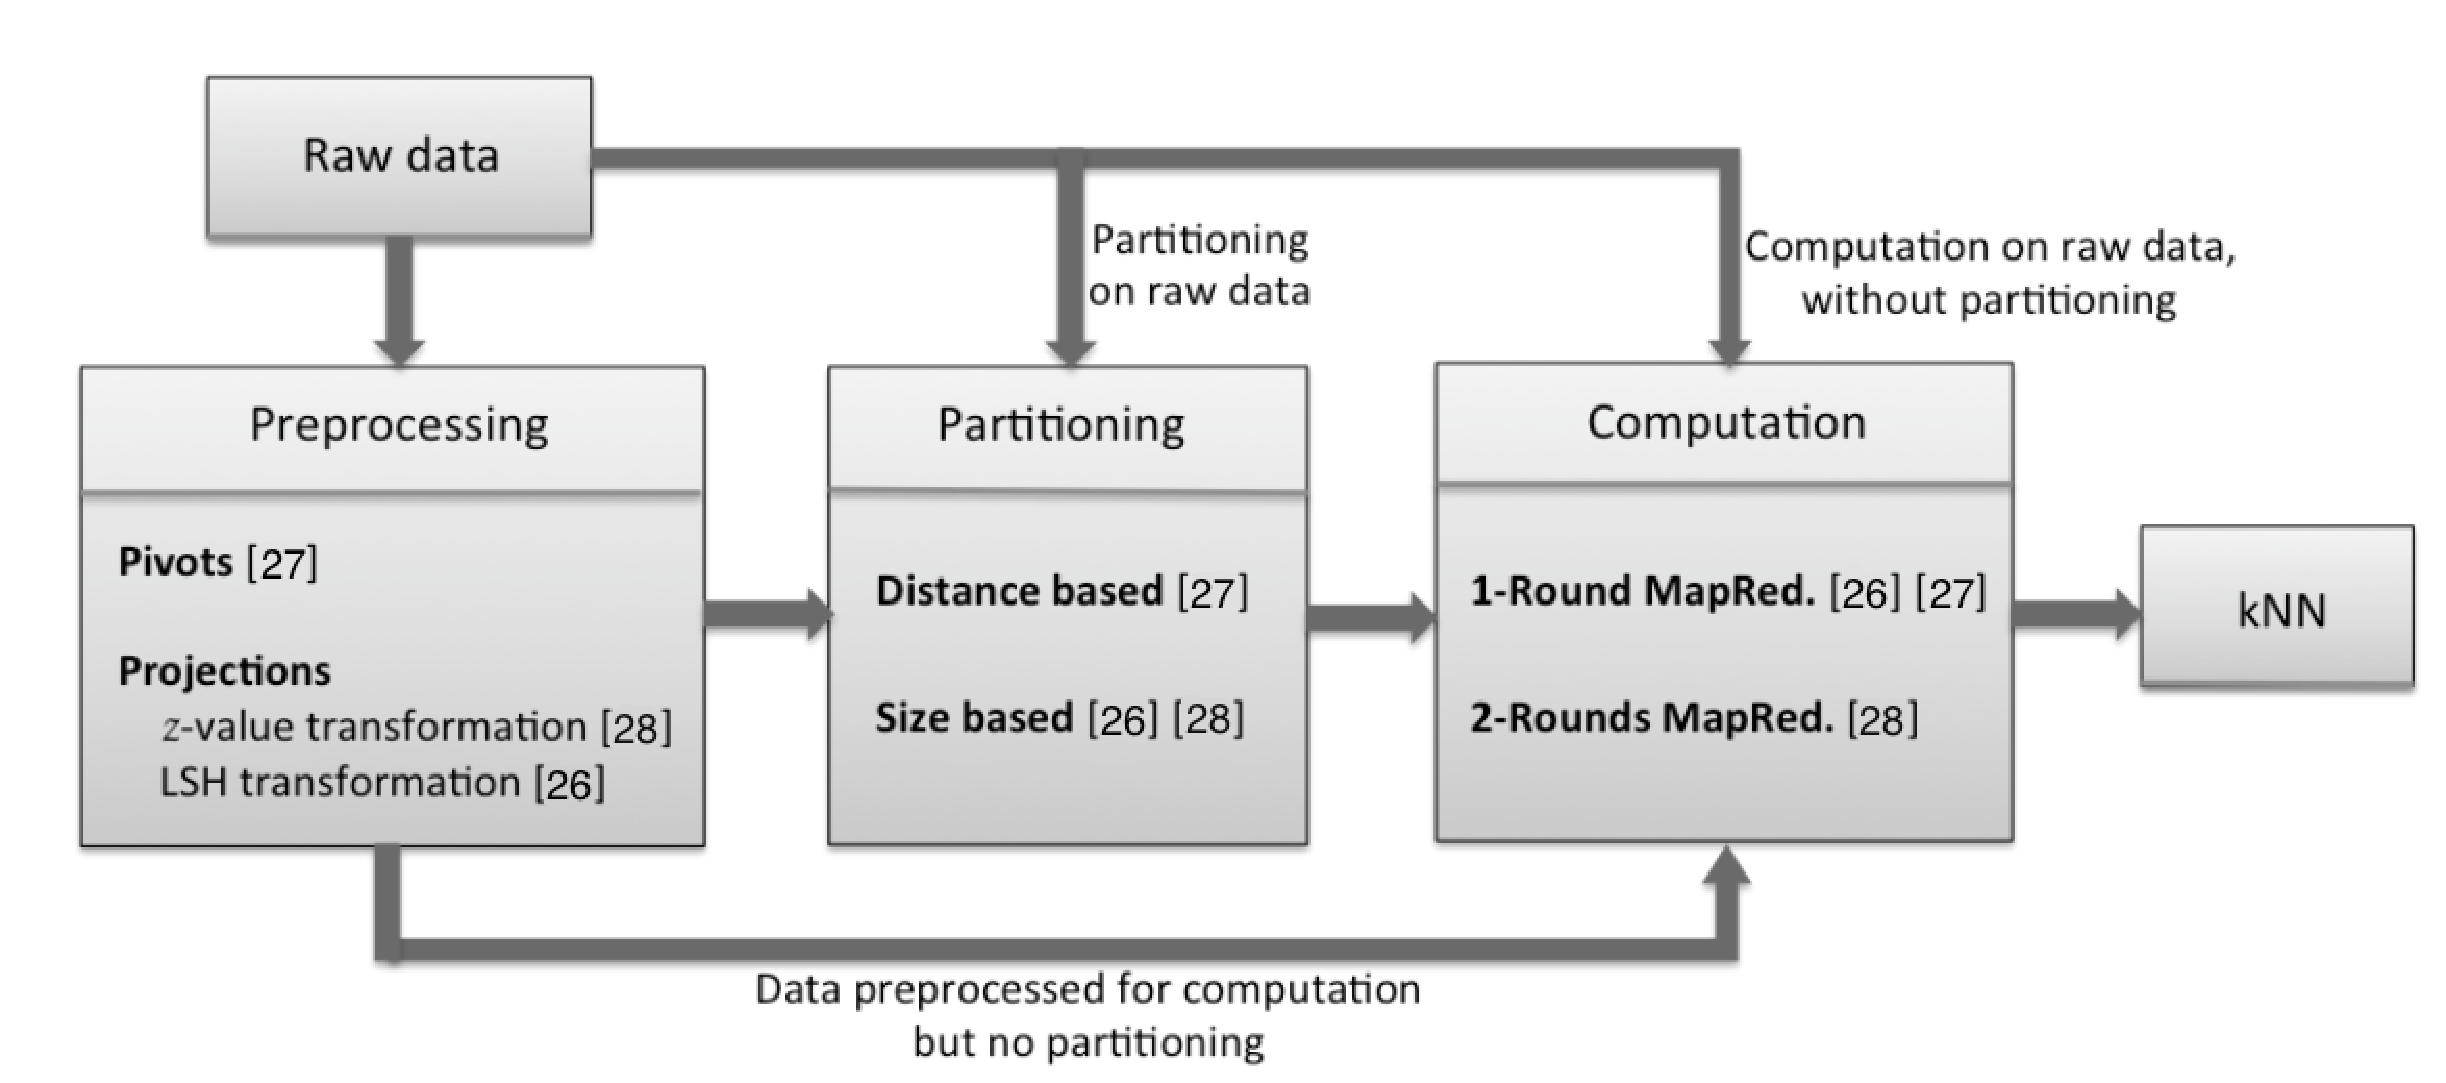
\includegraphics{workflow.pdf}}
\caption{Usual workflow of a kNN computation using MapReduce \label{workflow}}
\end{figure*}
Figure~\ref{workflow} summarizes the 
workflow we have gone through in this section and the techniques associated with each step.

%\subsection{Load Balance}
In a MapReduce job, the completion time of the Map phase and the Reduce phase depends on the longest-running task. This makes load balancing particularly 
important. In this sense, the partitioning strategy should ensure that the processing time of each task is roughly the same, so as to achieve the optimal 
overall 
performance. In our context, each task is used to calculate the pairwise distance of $<r_i, s_i>$ in the partition $<R_i, S_i>$. Thus, the number of distances that needs to be 
calculated is $\left| R_i \right|$ $\times$ $\left| S_i \right|$. If all tasks have to compute 
the same number of distances, they should have a roughly equivalent duration.  Hence, the optimal partition strategy should make:
\begin{center}
 $\forall$ i $\neq$ j, $\left| R_i \right|$ $\times$ $\left| S_i \right|$ = $\left| R_j \right|$ $\times$ $\left| S_j \right|$.
\end{center}

This is hard to ensure in practice. It is however possible
to obtain a sub-optimal solution in the following situation. Since 
$S_i$ is the set of possible nearest neighbors for the 
elements in $R_i$, then:
\begin{center}
$\forall$ i $\neq$ j, 

if $\left| R_i \right|$ = $\left| R_j \right|$ or $\left| S_i \right|$ = $\left| S_j \right|$, 

then $\left| R_i \right|$ $\times$ $\left| S_i \right|$ $\approx$ $\left| R_j \right|$ $\times$ $\left| S_j \right|$
\end{center} 
That is to say, if the number of objects in each partition of $R$ is equivalent, then the sum of the number of $k$ nearest neighbors of all objects in each partition can be considered approximately equivalent, and vice versa.

So an efficient partitioning should try to enforce either (1) $\left| R_i \right|$ = $\left| R_j \right|$ or (2) $\left| S_i \right|$ = $\left| S_j 
\right|$.
%When using space filling curves, the distance from the optimal solution (the true kNN) is often bounded, as explained in \cite{liao2001high}.

In \cite{Zhang:2012:EPK:2247596.2247602}, the authors give a short proof which 
shows that the worst-case complexity for (1) is equal to:
\begin{equation}
O\left(\left|R_i\right| \times log\left|S_i\right|\right) = O\left(\frac{\left|R\right|}{n} \times log\left|S\right|\right) \label{eq:complexity1}
\end{equation}


and for choice (2), the worst-case complexity is equal to:
\begin{equation}
O\left(\left|R_i\right| \times log\left|S_i\right|\right) = O\left(\left|R\right|\times log\frac{\left|S\right|}{n}\right) \label{eq:complexity2}
\end{equation}
where $n$ is the number of partitions. Since $n$~$\ll \left|S\right|$, the 
optimal partitioning is achieved when $\left| R_i \right|$ = $\left| R_j \right|$.


\subsection{Accuracy}
%Among the systems we have introduced, one crucial property that we have not 
%discussed yet is whether the system produces a reliable answer or not. In 
%order to quickly get answers, some systems prefer to loosen the accuracy of the 
%kNN computation. That is, in an approximate kNN computation, the results are 
%the same as in an exact kNN computation with a high probability. Nevertheless, results can be sub-optimal in some cases and even 
%incorrect with a low probability. This can be acceptable in situations where responsiveness is crucial, for example when there are user interactions. In 
%some other cases, only an exact 
%kNN computation is appropriate. Hence it is an important criteria, depending on the use cases.  

Usually, the lack of accuracy is the direct consequence of techniques such as  $z$-values and LSH used in the pre-processing step. In 
\cite{Zhang:2012:EPK:2247596.2247602} (H-zkNNJ), the authors show that when the dimension of the data increases, the quality of 
the results tends to decrease. This can be counterbalanced by increasing the number of random shifts applied to the data, thereby 
increasing the size of the resulting dataset. Experiments show that three 
shifts of the initial dataset (in dimension 15) are sufficient to achieve a good approximation 
(less than 10\% of errors shown in the experiences), while controlling the computation time. A similar result can be obtained with LSH by 
increasing the number of hash functions used. However, when using space filling curves, the distance from the optimal solution (the true kNN) is often bounded, which is not the case for LSH, as explained in \cite{liao2001high}.

%a consequence of a pre-processing step 
%performed to make the whole computation faster.
%
% Indeed, when dimensionality 
%increases, the distance between the nearest and the furthest neighbors tends to 
%decrease \cite{Beyer:1999:NNM:645503.656271}. This so called  
%\emph{curse of dimensionality} strongly influences the efficiency of tree-based exact kNN methods. 
%%\TODO{How? and why are we talking about centralized 
%%approaches here?}
%Also, dealing with data in high dimension greatly increases the complexity of the 
%partitioning and the computation of the distances. Many techniques such as 
%Voronoi-based diagrams or k-means, are in 
%theory applicable but become increasingly inefficient as the number of 
%dimensions increases. 
%
%Thus, one widely used method consists in reducing each point in the 
%data space into a point in a single dimension, while preserving the distance 
%relation between points. The representative techniques are $z$-values and LSH, as seen in the preprocessing section \ref{data_preprocessing}. 
%However this step cannot be performed without loss of precision, and 
%consequently the whole remaining process of the kNN computation suffers from 
%this reduction, possibly leading to incorrect results.
%
%In \cite{Zhang:2012:EPK:2247596.2247602} (H-zkNNJ), the authors reduce the dimension of 
%their data into one dimension, and are then able to partition 
%the data into intervals that contain the desired number of nearest neighbors. 
%By doing so, the authors gain one order of magnitude on the time needed 
%to compute approximate kNN compared to the most efficient exact solution they 
%found, and the gap tends to grow as the number of dimensions of the data 
%increases. However, when the dimension of the data increases, the quality of 
%the results tends to decrease, which they are able to counteract by 
%increasing the number of different shifts used to reduce the dimension of the 
%data to one dimension. The authors show in their experimentation that three 
%shifts of the initial dataset are sufficient to achieve a good approximation 
%(less than 10\% of errors shown in the experiences), while controlling the computation time.
%%\TODO{This 
%%is the z-value paper?Give more qualitative details maybe? do they 
%%theoretically estimate the error? What about the LSH paper? any result?}
%
%LSH is also one of the projection method aimed to transform data from high dimension to low dimension. The performance of LSH depends on parameter tuning. Like z-value method, we also need to process projection many times to increase the accuracy. But unlike z-value who generates some shifts of the original data, LSH will perform directly on the original data but with many hash functions.

%Although approximate, these solutions 
%are indeed fully usable in practice and can provide a high level of confidence, depending on the quality of results required by the application. 
%Nonetheless, error bounds are difficult nay impossible to compute, and mostly experiments enable to find the best parameters for a given approximate computation.
%\TODO{we need a better conclusion. Is there a bound or the error depends on the dataset? Is the gain always an order of magnitude? what is the cost of shifting?}

\section{Theoretical Analysis}\label{analysis}
\label{sec:analysis}
\subsection{Load Balance}
\label{sec:load_balance}
%MapReduce is a parallel and shared-nothing platforme.In Map Phase or Reduce Phase, each task will be done in parallel, so the computation time depends on the completion time of the longest task. 
In a MapReduce job, the Map tasks or the Reduce tasks will be processed in parallel, so the 
overall computation time of each phase depends on the completion time of the longest task. 
Therefore, in order to obtain the best performance, it is important that each task performs 
substantially the same amount of computation.  When considering load balancing in this section, we 
mainly want to have the same time complexity in each task. Ideally, we want to calculate roughly 
the same number of distance between $r_i$ and $s_j$ in each task.

For \HBK, there is no load balancing problem. Because in this basic method, only the Map Phase is treated in parallel. In Hadoop each task will process 64M data by default.

\HBNLJ~ cuts both the dataset $R$ and the dataset $S$ into $p$ equal-size pieces, then those pieces are 
combined pairwise to form a partition of $<R_i, S_j>$. Each task will process one block of data 
so we need to ensure that the size of the data block handled by each task is roughly the 
same. However, \HBNLJ~ uses a random partitioning method which can not exactly divide 
the data into equal-size blocks. 

\VO~ uses Voronoi diagram to cut the data space of $R$ into cells, where each cell is represented 
by its pivot. Then the data are assigned to the cell whose pivot is the nearest from it. For each 
$R$ cell, we need to find the corresponding pieces of data in $S$. Sometimes, the data in $S$ may be 
potentially needed by more than one $R$ cells, which will lead to the duplication of some 
elements of $S$. Thus the number of distances to be calculated in each task, i.e. the relative time 
complexity of each task is:
\begin{center}
$\mathcal{O}\left(Task\right)$ = $\left|P_i^R\right| \times \left(\left|P_i^S\right| + \left|RepS_c\right| \right)$
\end{center}
where $\left|P_i^R\right|$ and $\left|P_i^S\right|$ represents the number of elements in cell $P_i^R$ or 
$P_i^S$ respectively, and $\left|RepS_c\right|$ the number of replicated elements for the cell. 
Therefore, to ensure load balancing, we need to ensure that $\mathcal{O}\left(Task\right)$ is roughly the 
same for each task.
\VO~ introduces two methods to group the cells together to form a bigger cell which is the 
input of a task. \label{pgbj_grouping}
On one hand, the \emph{geo grouping} method supposes that close cells have a higher probability to 
replicate the same data. On the other hand, 
the \emph{greedy grouping} method estimates the cells whose data are more likely to be replicated. This approximation gives an upper bound on 
the complexity of the computation for a particular cell, which enables grouping of the cells that have the most replicated data in 
common. This leads to a minimization of replication and leads to groups that generate the same workload. 

And the \Z~ method assumes:

\begin{center}
$\forall$ i $\neq$ j, 

if $\left| R_i \right|$ = $\left| R_j \right|$ or $\left| S_i \right|$ = $\left| S_j \right|$, 

then $\left| R_i \right|$ $\times$ $\left| S_i \right|$ $\approx$ $\left| R_j \right|$ $\times$ $\left| S_j \right|$
\end{center} 
That is to say, if the number of objects in each partition of $R$ is equivalent, then the sum of 
the number of $k$ nearest neighbors of all objects in each partition can be considered 
approximately equivalent, and vice versa.
So an efficient partitioning should try to enforce either (i) $\left| R_i \right|$ = $\left| R_j 
\right|$ or (ii) $\left| S_i \right|$ = $\left| S_j 
\right|$.
In paper \cite{Zhang:2012:EPK:2247596.2247602}, the authors give a short proof which 
shows that the worst-case computational complexity for (i) is equal to:
\begin{equation}
\mathcal{O}\left(\left|R_i\right| \times log\left|S_i\right|\right) = \mathcal{O}\left(\frac{\left|R\right|}{n} \times log\left|S\right|\right) \label{eq:complexity1}
\end{equation}
and for choice (ii), the worst-case complexity is equal to:

\begin{equation}
\mathcal{O}\left(\left|R_i\right| \times log\left|S_i\right|\right) = \mathcal{O}\left(\left|R\right|\times log\frac{\left|S\right|}{n}\right) \label{eq:complexity2}
\end{equation}
where $n$ is the number of partitions. Since $n$~$\ll \left|S\right|$, the 
optimal partitioning is achieved when $\left| R_i \right|$ = $\left| R_j \right|$.

In \LSH, a custom partitioner is used to load balance tasks between reducers. Let $W_{h}=\mid R_{h} \mid \times \mid S_{h} \mid$ be the weight of bucket $h$. A bin packing algorithm is used such that each reducer ends up 
with approximately the same amount of work. More precisely, let $\mathcal{O}\left(R_i\right)  = \sum_{h}{W_{h}}$ the
work done by reducer $R{i}$, then this methods guarantees that 
\begin{equation}
\forall i \neq j, \mathcal{O}\left(R_i\right)  \approx  \mathcal{O}\left(R_j\right)
\end{equation}
Because the weight of a bucket is only an approximation of the computing time, this method can only give an
approximate load balance. Having a large number of buckets compared to the number of reducers significantly improves
the load balancing.   


\subsection{Accuracy}

Usually, the lack of accuracy is the direct consequence of techniques to reduce the 
dimensionality with techniques such as $z$-values and LSH. In 
\cite{Zhang:2012:EPK:2247596.2247602} (\Z), the authors show that when the dimension of the 
data increases, the quality of 
the results tends to decrease. This can be counterbalanced by increasing the number of random 
shifts applied to the data, thereby 
increasing the size of the resulting dataset. Their experiments show that three 
shifts of the initial dataset (in dimension 15) are sufficient to achieve a good approximation 
(less than 10\% of errors measured), while controlling the computation time. 
Furthermore, paper \cite{5447837_full} shows a detailed theoretical analyses showing that, for any fixed dimension, by using only $\mathcal{O}$(1) random shifts of data, the $z$-value method returns a constant factor approximation in terms of the radius of the $k$ nearest neighbor ball.

For LSH, the accuracy is defined by the probability that the method will return the real nearest neighbor. Suppose that 
the points within a distance $d = \left|p-q\right|$ are considered as close points. The probability \cite{4472264} that 
these two points end up in the same bucket is: 
\begin{equation}
p(d) = Pr_\mathcal{H}\left[h(p)=h(q)\right] \\
=\int_{0}^{W} \frac{1}{d} f_s (\frac{x}{d})(1-\frac{x}{W})dx
\end{equation}
where W is the size of the bucket and $f_s$ is the probability density function of the hash function $\mathcal{H}$. 
From this equation we can see that for a given bucket size W, this probability decreases as the distance $d$ 
increases. Another way to improve the accuracy of LSH is to increase the number of hashing families
used. The use of LSH in \LSH~has an interesting consequence on the number of results. Depending on the parameters, 
the number of elements in a bucket might be smaller than $k$. 
Overall, unlike $z$-value, the performance of LSH depends a lot on parameter tuning. 
%\subsection{Complexity}
\begin{figure*}[t]
\center
\scalebox{0.6}{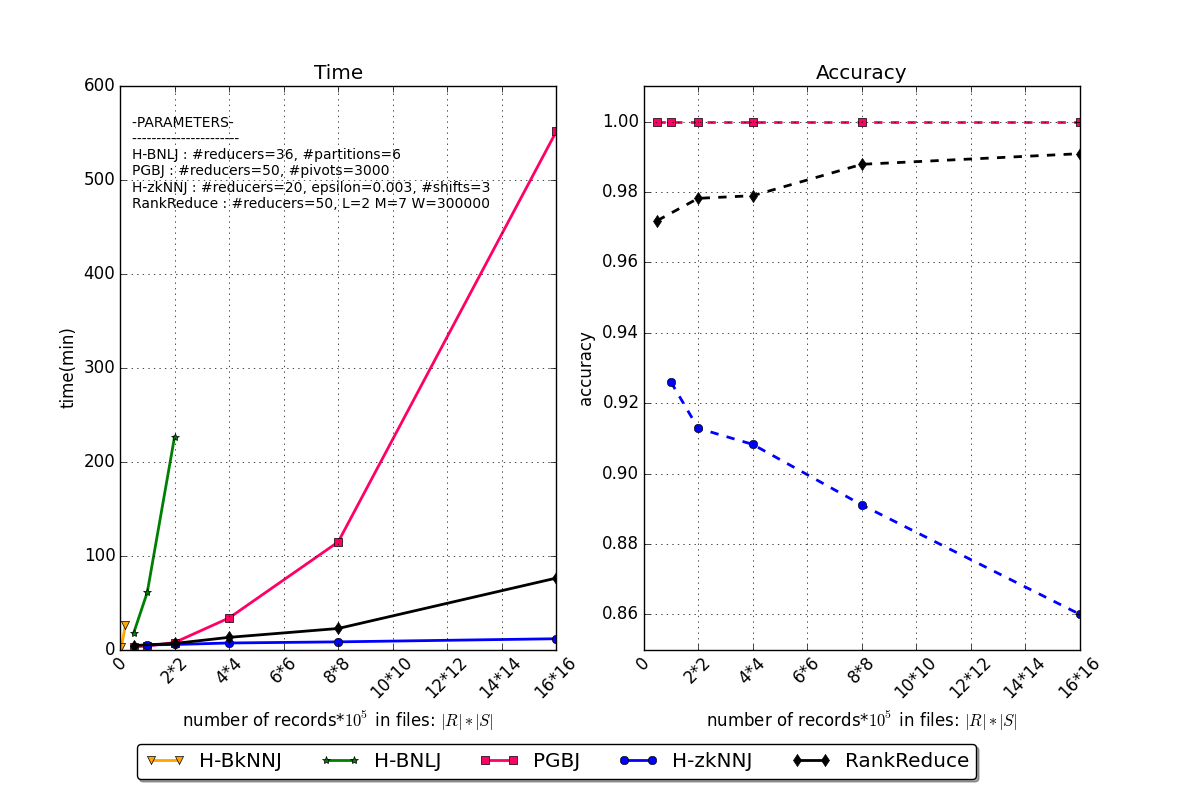
\includegraphics{res/time.png}}
\caption{Completion time and accuracy of knn mapreduce algorithms\label{experiment}}
\end{figure*}
Computational complexity is often used to describe the execution time of an algorithm. When computing kNN with MapReduce, additional factors strongly impact the execution time: 
\begin{itemize}

\item[(1)] \textbf{The number of MapReduce jobs:} Starting a job (whether in 
Hadoop\cite{Jiang:2010:PMI:1920841.1920903} or any other platform) requires some initialization steps 
such as allocating resources and copying data. Those steps can be very time 
consuming.

\item[(2)] \textbf{The number of Map tasks and Reduce tasks used to calculate kNN$\left(R_i \ltimes S\right)$:} The larger this number is, the more 
information is exchanged through the network during the Shuffle phase. 
Moreover, scheduling a task also incurs an overhead.

\item[(3)] \textbf{The number of distances to compute and to sort for each object $r_i$:} Sorting is a dominating operation, so the number of elements to be 
sorted also impacts computation time.
\end{itemize} 

%Here, we analyze the previously described systems 

The basic method H-BkNNJ only uses one MapReduce job, and requires  
$n^2$ Map tasks to calculate the distances where $n$ is the number of 
partitions. The complexity of sorting all distances for one  $r_i$ in $R$ is $
\left|S\right| \times log\left|S\right|$. Since $S$ is usually a large 
dataset, this method quickly becomes impracticable.

To overcome this limitation, H-BNLJ or H-BRJ \cite{Zhang:2012:EPK:2247596.2247602} uses 2 MapReduce jobs, again 
with $n^2$ Map tasks to compute the distances. However, using of a second 
job significantly reduces the complexity of sorting  to $\left|n \cdot k
\right| \times log\left|n \cdot k\right|$, where $n$ is the number of 
partitions and $k$ is the number of nearest neighbors 
queried.

PGBJ\cite{Lu:2012:EPK:2336664.2336674} performs a pre-processing phase followed by 2 MapReduce jobs. This method also 
only uses $n$ Map tasks to calculate the distances. Overall, the sorting complexity is reduced to $\left|S_i\right| \times log\left|S_i\right|$. 

H-zkNNJ\cite{Zhang:2012:EPK:2247596.2247602} also begins by a pre-processing phase and uses in total 3 MapReduce jobs in 
exchange for taking only $n$ Map tasks to compute the distances. Moreover, they only take $
\left(r_i, C_i\left(r_i\right)\right)$, that is the candidate neighbors set, into account. Since $C_i\left(r_i\right)$ contains only $2k$ neighbors for each  
$r_i$, the complexity is now reduced to $\left|2 \cdot k\right| \times log\left|2 \cdot k\right|$.
\subsection{Global Complexity}
\label{section:global_complexity}
Carefully balancing the number of jobs, tasks, computation and communication 
is an important part of designing an efficient distributed algorithm.
All the $k$NN algorithms studied in this survey have different characteristics. We will now describe them 
and outline how they can impact the execution time. 

\begin{itemize}
\item[(1)] \textbf{The number of MapReduce jobs:} Starting a job (whether in 
Hadoop\cite{Jiang:2010:PMI:1920841.1920903} or any other platform) requires some initialization steps 
such as allocating resources and copying data. Those steps can be very time 
consuming.
\item[(2)] \textbf{The number of Map tasks and Reduce tasks used to calculate $k$NN$\left(R_i \ltimes S\right)$:} The 
larger this number is, the more 
information is exchanged through the network during the shuffle phase. 
Moreover, scheduling a task also incurs an overhead. But the smaller this number is, the more computation is done by 
one machine.
\item[(3)] \textbf{The number of final candidates for each object $r_i$:
%\sout{ i.e each r of original dataset R:}
} %Sorting is 

We have seen that advanced algorithms use pre-processing and partitioning techniques to reduce this number as much as possible. The goal
is to reduce the amount of data transmitted and the computational cost. 


\end{itemize} 

 

Together these three points impact two main overheads that affect the performance:
\begin{itemize}
\item Communication overhead, which can be considered as the amount of data transmitted over the network during the 
shuffle phases. 

\item Computation overhead, which %which is the CPU overhead used to calculate by each task. This overhead 
is mainly composed of two parts: 1). computing the distances, 2). finding the $k$ smallest distances. It is also 
impacted by the complexity (dimension) of the data.
\end{itemize}

 

Suppose the dataset is $d$ dimensional, the overhead for computing the distance is roughly the same for every $r_i$ and 
$s_j$ for each method. The difference comes from the number of distances to 
sort for each element $r_i$ to get the top $k$ nearest neighbors. Suppose that the dataset $R$ is divided into $n$ splits. 
Here $n$ represents the number of partitions of $R$ and $S$ for \HBNLJ~ and \Z, the number of cells after using the 
grouping strategy for \VO~ and the number of buckets for \LSH. %the number of tasks can be represented by $n$.
Assuming there is a good load balance for each method, the number of elements in one split $R_i$ can be 
considered as $\frac{\left|R\right|}{n}$. Finding the $k$ closest neighbors efficiently for a given $r_i$ can be done using 
a priority queue, which less costly than sorting all candidates.


%Here we go through the details for each methods.
Since all these algorithms uses different strategies, their steps cannot be directly compared. Nonetheless,
to provide a theoretical insight, we will now compare their complexity for the last phase, which is common to all of 
them. 


The basic method \HBK~only uses one MapReduce job, and requires  
only one Reduce task to compute and sort the distances. The communication overhead is $\mathcal{O} 
(\left|R\right|+\left|S\right|)$. The number of final candidates for one $r_i$ is $|S|$. The complexity of finding the 
$k$ smallest distances for $r_i$ is $\mathcal{O}(
\left|S\right| \cdot log\left(k\right))$. Hence, the total cost for one task is $\mathcal{O}(\left|R\right| 
\cdot \left|S\right| \cdot \log\left(k\right))$. Since $R$ and $S$ are usually large 
datasets, this method quickly becomes impracticable.

To overcome this limitation,  {\bf \HBNLJ}  \cite{Zhang:2012:EPK:2247596.2247602} uses two MapReduce jobs, with $n^2$  
tasks 
to compute the distances.
Using a second  job significantly reduces the number of final candidates to $nk$. 
The total communication overhead is $\mathcal{O}(n\left|R\right|+n\left|S\right|+kn\left|R\right|)$. The 
complexity of finding the $k$ elements for each $r_i$ is reduced to $\left(n \cdot k
\right) \cdot log\left(k\right)$. Since each task has $\frac{\left|R\right|}{n}$ elements, the total sort overhead for 
one task is $\mathcal{O}(\left|R\right| \cdot k \cdot log(k))$.


{\bf \VO} \cite{Lu:2012:EPK:2336664.2336674} performs a preprocessing phase followed by two MapReduce jobs. This method 
also 
only uses $n$ Map tasks to compute the distances and the number of final candidates falls to $|S_i|$. Since this method 
uses a distance based partitioning method, 
the size of $|S_i|$ varies, depending on the number of cells
required to perform the computation and the number of replications ($\left|RepS_c\right|$, see 
Section~\ref{sec:load_balance}) required by each cell. As 
such, the computational complexity cannot be expressed easily.%\TODO{Check in the original paper what the authors say about this}. 
%It equals to the sum of the number of data in the cells of this group additionally to the dataset $S$ replicated 
%inside of this group.
%For one group, PGBJ sorts its cells to avoid to search in all the dataset $S_i$ thanks to a threshold. In worst case, 
%per one $r_i$, its computing becomes $|S_i|*log(k)$. In the best case its search only in its own cells.
Overall, finding
the $k$ elements is reduced to $\mathcal{O}(\left|S_i\right| \cdot log\left|k\right|)$ for each $r_i$, and 
$\mathcal{O}(\frac{\left|R\right|}{n} \cdot \left|S_i\right| \cdot log\left|S_i\right|)$ in total per task.
 The communication overhead is $\mathcal{O}(\left|R\right| + \left|S\right| + \left|RepS_c\right|\cdot n)$. In the 
 original 
paper the authors gives a formula to compute $\left|RepS_c\right|\cdot n$, which is the total number of 
replications for the whole dataset $S$. %, and the authors gives a formulation for 

In {\bf \LSH} \cite{Stupar10rankreduce-}, the initial dataset is projected by $L$ hash  families into 
buckets.
After finding the local candidates in the second job, the third job combines the local results to 
find the global $k$ nearest neighbor. For each $r_i$, the number of final candidates is $L\cdot k$. Finding the $k$ 
elements takes $\mathcal{O}(L \cdot k \cdot log(k))$ per $r_i$, and $\mathcal{O}(|R_i| \cdot L \cdot k \cdot log(k))$ 
per task. The total communication cost becomes $\mathcal{O}(|R|+|S|+k\cdot |R|)$.



{\bf \Z}\cite{Zhang:2012:EPK:2247596.2247602} also begins by a preprocessing phase and uses in total three MapReduce 
jobs in exchange for requiring only $n$ Map tasks. For a given $r_i$, these tasks 
process elements from the candidate neighbor set $C\left(r_i\right)$. By construction, $C\left(r_i\right)$ only 
contains  $\alpha \cdot k$ neighbors, where $\alpha$ is the number of shifts of the original dataset. The complexity is now reduced to $\mathcal{O}(\left(\alpha \cdot k\right) \cdot log\left(k\right))$ for one $r_i$, 
and $\mathcal{O}(\frac{\left|R\right|}{n} \cdot \left(\alpha \cdot k\right) \cdot log\left(k\right))$ in total 
per task. The communication overhead is 
$\mathcal{O}(\frac{1}{\varepsilon^2}+\left|S\right|+k \cdot \left|R\right|)$, with $\varepsilon \in (0,1)$, a parameter
of the sampling process. \\

From the above analysis we can infer the following. \HBK~only uses one task, but this task needs to calculate the 
entire data set. 
\HBNLJ~uses $n^2$ tasks to greatly reduce the amount of data processed by each task. However this also increases the 
amount of data to be exchanged among the nodes. This should prove to be a major bottleneck. 
\VO, \LSH~and \Z~all use three jobs which reduces the number of tasks to $n$, and thus reduces the communication 
overhead.

Although the computational complexity 
of each task depends on various parameters of the preprocessing phases, it is possible to outline a partial 
conclusion from this analysis. There are basically three performance brackets. First, the least efficient should be 
\HBK, followed by \HBNLJ. \VO, \LSH~and 
\Z~are theoretically the most efficient. Among them, \VO~has the largest number of final candidates. For \LSH~and
\Z~, the number of final candidates is of the same order of magnitude. The main difference lies in the communication
complexity, more precisely in $\frac{1}{\varepsilon^2}$ compared to $\left|R\right|$. As the dataset size increases,
we will have eventually  $\left|R\right| \gg \frac{1}{\varepsilon^2}$. Hence, \Z~seems to be the theoretically most
efficient for large query sets.

%%\begin{table*}[htp]
%\centering
%\begin{tabular}{|c|c|c|c|c|c|c|}
%\hline
%\multirow{2}{*}{\textbf{Systems}}  & \multirow{2}{*}{\textbf{Preprocessing}} & \multirow{2}{*}{\textbf{Partitioning}}                                              
%& \multirow{2}{*}{\textbf{Accuracy}} & \multicolumn{3}{c|}{\textbf{Complexity}} \\ \cline{5-7} 
%                                                                     &                                                                         &                                                                            & \multicolumn{1}{l|}{}                          & \textbf{Total Jobs} & \textbf{Tasks}               & \textbf{Sort}                                           \\ \hline
%\begin{tabular}[c]{@{}c@{}}\textbf{H-BkNNJ}\\ (Basic Method)\end{tabular}     & None                                                                    & None                                                                       & Exact                                          & 1          & 1                   & $\left|S\right| \times log\left|S\right|$                 \\ \hline
%\begin{tabular}[c]{@{}c@{}}\textbf{H-BNLJ} \cite{Zhang:2012:EPK:2247596.2247602} \\ (Zhang et al.)\end{tabular}      & None                                                                    & None                                                                       & Exact                                          & 2          & $p^2$ & $\left(n \cdot k\right) \times log\left(n \cdot k\right)$ \\ \hline
%\begin{tabular}[c]{@{}c@{}}\textbf{PGBJ} \cite{Lu:2012:EPK:2336664.2336674}\\ (Luet al.)\end{tabular}            & \begin{tabular}[c]{@{}c@{}}Pivots\\ Selection\end{tabular}              & \begin{tabular}[c]{@{}c@{}}Distance Based\\ (Voronoi Diagram)\end{tabular} & Exact                                          & 3          & $\left|grouping\right|$                   & $\left|S_i\right| \times log\left|S_i\right|$             \\ \hline
%\begin{tabular}[c]{@{}c@{}}\textbf{RankReduce} \cite{Stupar10rankreduce-}\\ (Stupar et al.)\end{tabular} & LSH                                                                     & Size Based                                                                 & Approximate                                    & 3           & $\left|buckets\right|$   & $\left(L \cdot k\right) \times log\left(L \cdot k\right)$ \\ \hline
%\begin{tabular}[c]{@{}c@{}}\textbf{H-zkNNJ} \cite{Zhang:2012:EPK:2247596.2247602}\\ (Zhang et al.)\end{tabular}     & \begin{tabular}[c]{@{}c@{}}Z-Value\\ (Space Filling\\ Curve)\end{tabular} & Size Based                                                                 & Approximate                                    & 3          & n                  & $\left(2 \cdot k\right) \times log\left(2 \cdot k\right)$ \\ \hline
%\end{tabular}
%\caption{Summary table of kNN computing systems with MapReduce \TODOREP{(qui est n qui est i ect....)}}\label{summary_table}
%\end{table*}


% Please add the following required packages to your document preamble:
% \usepackage{multirow}
\begin{table*}[htp]
\centering
\renewcommand{\arraystretch}{1.3} 
\begin{tabular}{|c|c|c|c|c|c|c|c|}
\hline
\multirow{4}{*}{\centering{ \bf Methods}}                                            & \multirow{4}{*}{\centering{\textbf{Preprocessing}}}                                & 
\multirow{4}{*}{\centering{\textbf{Partitioning}}}                                   &
\multirow{4}{*}{\centering{\textbf{Accuracy}}} &
\multicolumn{4}{c|}{\textbf{Complexity}}                                                                                \\ \cline{5-8} 
                                                                              &                                                                           &                                                                            &                                    & \textbf{Jobs} & \textbf{Tasks}   &\textbf{\begin{tabular}[c]{@{}c@{}} Final\\ Candidate \\ (per $r_i$)\end{tabular}} & \multicolumn{1}{c|}{\textbf{Communication}} \\ \hline
\begin{tabular}[c]{@{}c@{}}\textbf{H-BkNNJ}\\ (Basic Method)\end{tabular}    & None                                                                      & None                                                                       & Exact                              & 1             & 1                                                      &                                           $|S|$                                   &                                            $\mathcal{O} (\left|R\right|+\left|S\right|)$ \\ \hline
\begin{tabular}[c]{@{}c@{}}\textbf{H-BNLJ} \cite{Zhang:2012:EPK:2247596.2247602} \\ (Zhang et al.)\end{tabular}      & None                                                                      & None                                                                       & Exact                              & 2             & $n^2$  & $nk$                                   &                \begin{tabular}[c]{@{}c@{}}                            $\mathcal{O}(n\left|R\right|$ \\
$+n\left|S\right|+kn\left|R\right|)$ \end{tabular} \\ \hline
\begin{tabular}[c]{@{}c@{}}\textbf{PGBJ} \cite{Lu:2012:EPK:2336664.2336674}\\ (Lu et al.)\end{tabular}             & 
\begin{tabular}[c]{@{}c@{}}Pivots\\ Selection\end{tabular}                & \begin{tabular}[c]{@{}c@{}}Distance \\ 
Based\end{tabular} & Exact                              & 3             & 
n                                                     &  $\left|S_i\right|$                                   & 
\begin{tabular}[c]{@{}c@{}}                                  $\mathcal{O}(\left|R\right|$ \\
$ + \left|S\right| + \left|RepS_c\right|\cdot n)$ \end{tabular}                                    \\ \hline
\begin{tabular}[c]{@{}c@{}}\textbf{\LSH} \cite{Stupar10rankreduce-}\\ (Stupar et al.)\end{tabular} & 
LSH                                                                       & Size 
Based                                                                 & Approximate                        & 
3             & n                   & 
\begin{tabular}[c]{@{}c@{}}
$L \cdot k $
\end{tabular}                            &           \begin{tabular}[c]{@{}c@{}}   $ \mathcal{O}(|R|+|S|$ \\ $+ 
k \cdot |R|)$          \end{tabular}                     \\ \hline
\begin{tabular}[c]{@{}c@{}}\textbf{H-zkNNJ} \cite{Zhang:2012:EPK:2247596.2247602}\\ (Zhang et al.)\end{tabular}    & 
\begin{tabular}[c]{@{}c@{}}Z-Value\end{tabular} & Size 
Based                                                                 & Approximate                        & 
3             & n                  & \begin{tabular}[c]{@{}c@{}}$\alpha \cdot k 
$\end{tabular}                                   &    $\mathcal{O}(\frac{1}{\varepsilon^2}+\left|S\right|+k \cdot 
\left|R\right|)$                                         \\ \hline
\end{tabular}
\caption{Summary table of kNN computing systems with MapReduce
%\TODOREP{Y'a encore des erreurs !!! pour z la dernire phase t'as juste $shift*k$ candidates c'est ds la phase 2 ou tu extrait $2*k$. communication overhead pour Zvalue est fausse aussi.
%en plus ca apporte rien si au moins on rajoute une cologne intermediate candidate.
%Apres pour PGBJ vous mettez 1 colonne pas deux ainsi que pour HBKNNJ
%}
\label{summary_table_new}
}
\end{table*}


\begin{table*}[htp]
\centering
\renewcommand{\arraystretch}{1.3} 
\begin{tabular}{|c|c|c|c|c|c|c|c|}
\hline
\multirow{4}{*}{\centering{ \bf Methods}}                                            & \multirow{4}{*}{\centering{\textbf{Preprocessing}}}                                & 
\multirow{4}{*}{\centering{\textbf{Partitioning}}}                                   &
\multirow{4}{*}{\centering{\textbf{Accuracy}}} &
\multicolumn{4}{c|}{\textbf{Complexity}}                                                                                \\ \cline{5-8} 
                                                                              &                                                                           &                                                                            &                                    & \textbf{Jobs} & \textbf{Tasks}   &\textbf{\begin{tabular}[c]{@{}c@{}} Final\\ Candidate \\ (per $r_i$)\end{tabular}} & \multicolumn{1}{c|}{\textbf{Communication}} \\ \hline
\begin{tabular}[c]{@{}c@{}}\textbf{H-BkNNJ}\\ (Basic Method)\end{tabular}    & None                                                                      & None                                                                       & Exact                              & 1             & 1                                                      &                                           $|S|$                                   &                                            $\mathcal{O} (\left|R\right|+\left|S\right|)$ \\ \hline
\begin{tabular}[c]{@{}c@{}}\textbf{H-BNLJ} \cite{Zhang:2012:EPK:2247596.2247602} \\ (Zhang et al.)\end{tabular}      & None                                                                      & None                                                                       & Exact                              & 2             & $n^2$  & $nk$                                   &                \begin{tabular}[c]{@{}c@{}}                            $\mathcal{O}(n\left|R\right|$ \\
$+n\left|S\right|+kn\left|R\right|)$ \end{tabular} \\ \hline
\begin{tabular}[c]{@{}c@{}}\textbf{PGBJ} \cite{Lu:2012:EPK:2336664.2336674}\\ (Lu et al.)\end{tabular}             & 
\begin{tabular}[c]{@{}c@{}}Pivots\\ Selection\end{tabular}                & \begin{tabular}[c]{@{}c@{}}Distance \\ 
Based\end{tabular} & Exact                              & 3             & 
n                                                     &  $\left|S_i\right|$                                   & 
\begin{tabular}[c]{@{}c@{}}                                  $\mathcal{O}(\left|R\right|$ \\
$ + \left|S\right| + \left|RepS_c\right|\cdot n)$ \end{tabular}                                    \\ \hline
\begin{tabular}[c]{@{}c@{}}\textbf{\LSH} \cite{Stupar10rankreduce-}\\ (Stupar et al.)\end{tabular} & 
LSH                                                                       & Size 
Based                                                                 & Approximate                        & 
3             & n                   & 
\begin{tabular}[c]{@{}c@{}}
$L \cdot k $
\end{tabular}                            &           \begin{tabular}[c]{@{}c@{}}   $ \mathcal{O}(|R|+|S|$ \\ $+ 
k \cdot |R|)$          \end{tabular}                     \\ \hline
\begin{tabular}[c]{@{}c@{}}\textbf{H-zkNNJ} \cite{Zhang:2012:EPK:2247596.2247602}\\ (Zhang et al.)\end{tabular}    & 
\begin{tabular}[c]{@{}c@{}}Z-Value\end{tabular} & Size 
Based                                                                 & Approximate                        & 
3             & n                  & \begin{tabular}[c]{@{}c@{}}$\alpha \cdot k 
$\end{tabular}                                   &    $\mathcal{O}(\frac{1}{\varepsilon^2}+\left|S\right|+k \cdot 
\left|R\right|)$                                         \\ \hline
\end{tabular}
\caption{Summary table of kNN computing systems with MapReduce
%\TODOREP{Y'a encore des erreurs !!! pour z la dernire phase t'as juste $shift*k$ candidates c'est ds la phase 2 ou tu extrait $2*k$. communication overhead pour Zvalue est fausse aussi.
%en plus ca apporte rien si au moins on rajoute une cologne intermediate candidate.
%Apres pour PGBJ vous mettez 1 colonne pas deux ainsi que pour HBKNNJ
%}
\label{summary_table_new}
}
\end{table*}

%\vspace{-0.25cm}
\subsection{Wrap up}
Although the workflow for computing kNN on MapReduce is the same for all existing solutions, the guarantees offered by each of them vary a lot. As load 
balancing is a key point to shrink completion time, one should carefully choose the partitioning method to achieve this goal. Also, the accuracy of the 
computing system is crucial: are exact results really needed? If not, then one might trade accuracy for efficiency, by using data transformation 
techniques before the actual computation. 
Complexity of the global system should also be taken into account for particular needs, although it is often related to the accuracy: an exact system is 
usually more complex than an approximate one.
Finally, none of the systems really offers a way to handle data updates. This is due to the specific partitioning performed before computing. Indeed, an 
efficient partitioning is adapted to a particular dataset, and might not be adapted to another.
Table~\ref{summary_table} is a summary table of the systems we have examined and their main characteristics.



\subsection{Wrap up}
Although the workflow for computing kNN on MapReduce is the same for all existing solutions, the guarantees offered by each of them vary a lot. As load 
balancing is a key point to reduce completion time, one should carefully choose the partitioning method to achieve this goal. Also, the accuracy of the 
computing system is crucial: are exact results really needed? If not, then one might trade accuracy for efficiency, by using data transformation 
techniques before the actual computation. 
Complexity of the global system should also be taken into account for particular needs, although it is often related to the accuracy: an exact system is 
usually more complex than an approximate one.
Table~\ref{summary_table_new} shows a summary of the systems we have examined and their main characteristics.

Due to the multiple parameters and very different steps for each algorithm, we had to limit our complexity analysis to 
common operations. Moreover, for some of them, the complexity depends on parameters set by a user or some properties
of the dataset. Therefore, the total processing time might be different, in practice, than the one predicted by the 
theoretical analysis. That is why it is important to have a thorough experimental study.

%\section{Evaluation}\label{evaluation}
In order to compare theoretical performance and performance in practice, we performed an extensive experimental evaluation of the algorithms described in the 
previous sections.

The experiments were run on two clusters of Grid'5000\footnote{\url{www.grid5000.fr}}, one with Opteron 2218 processors 
and 8GB of memory, the other with Xeon E5520 processors and 32GB of memory, using Hadoop 1.3, 1Gb/s Ethernet and SATA hard drives. %\TODO{hard disk type, 
%ethernet. . Not useful, too much details}. 
We follow the default configuration of 
Hadoop: (1) the number of 
replications for each split of data is set 
to 3; (2) the number of slot of each node is 1, so only one map/reduce task is processed on the node at one time.
%\TODO{(3) the virtual memory for each map/reduce tasks is: xxx}

We evaluate the five approaches presented before.
% following approaches in the experiments.
%
%\begin{itemize}
%
%\item \textbf{H-BkNNJ:} the naive method.
%
%\item \textbf{H-BNLJ:} the block nested loop method.
%
%\item \textbf{PGBJ:} the method using Voronoi Diagram to partition data
%
%\item \textbf{RankReduce:} the method using LSH to reduce the dimension of data
%
%\item \textbf{H-zkNNJ:} the method using z-value to reduce the dimension of data
%
%\end{itemize}

 For \Z~and \HBNLJ, we took the source code provided by the authors as a starting 
point\footnote{\url{http://ww2.cs.fsu.edu/~czhang/knnjedbt/}} and added some modifications to reduce the size of 
intermediate files. The others were implemented from scratch using the 
description provided in their respective papers.

When implementing \LSH, we added a reduce phase to the first MapReduce job to compute some statistics information for 
each bucket. These information is used for achieving good load balance. %Using these statistics, a custom partitioner 
%distributes buckets among the 
%reducers to try to achieve good work balance. 
Moreover, in the original version, the authors only use one 
hash function. To improve the precision, we choose to use multiple families and hash functions depending on the 
dataset. Finally, our version of \LSH~ uses three MapReduce jobs instead of two.

Most of the experiments were ran using two different datasets: 

\begin{itemize}

\item \textbf{OpenStreetMap: }we call it the \emph{Geographic - or Geo - dataset}. The Geo dataset  
involves geographic XML data in two dimensions\footnote{Taken from: \url{http://www.geofabrik.de/data/download.html}}. 
This is a real dataset containing the location and description of objects. The data is organized by region. We extract 
$256*10^5$ records from the region of France.

\item \textbf{Catech 101: }we call it the \emph{Speeded Up Robust Features - or SURF - dataset}. It is a public set of images\footnote{Taken from: \url{www.vision.caltech.edu/Image_Datasets/Caltech101}}, which contains 101 categories of pictures of objects, and 40 to 800 images per category. 
SURF\cite{Surf} is a detector and a descriptor for points of interest in images, which produces image data
%Image feature descriptors are known to be high dimensional data, so we chose to use SURF\cite{Surf}, which produces image data
in 128 dimensions.  We extract 32 images per category, each image has between 1000 and 2000 descriptors.

\end{itemize}

In order to learn the impact of dimension and dataset, we use 5 additional datasets: \textbf{El Nino: } in 9 dimensions; \textbf{HIGGS: } in 28 dimensions; \textbf{TWITTER: } in 77 dimensions; \textbf{BlogFeedBack: } in 281 dimensions; and \textbf{Axial Axis: } in 386 dimensions. These data sets are all downloaded from UCI Machine Learning Repository\footnote{Taken from: \url{https://archive.ics.uci.edu/ml/}}.

%In order to learn the impact of dimension and dataset, we also use: \textbf{El Nino: }(in 9 dimensions) consists of nearly 70 moored buoys spanning the equatorial Pacific to measure oceanographic and surface meteorological variables; \textbf{HIGGS: }(in 28 dimensions) has been produced using Monte Carlo simulations, where the first 21 features (columns 2-22) are kinematic properties and the last seven features are functions of the first 21 features  to help discriminate between the two classes; \textbf{TWITTER: }(in 77 dimensions) contains two different social networks Tom’s Hardware (TH) (41 million visitors per month) and Twitter (TW) (500 million visitors per month); \textbf{SIFT: }(in ) \TODO{I didn't find any description}; \textbf{BlogFeedBack: }(in 281 dimensions) originates from blog posts; and \textbf{Axial Axis: }(in 386 dimensions) was retrieved from a set of 53500 CT images from 74 different 
%patients (43 male, 31 female). These data sets are all downloaded from UCI Machine Learning Repository\footnote{Taken from: \url{https://archive.ics.uci.edu/ml/}}.

We use a self-join for all our experiments, which means we use two datasets of equal sizes for $R$ and $S$ 
($|R|=|S|$). We also vary the number of 
records of each dataset from $0.125*10^5$ to $256*10^5$.
For all experiments, we have set $k=20$ unless specified otherwise. 
%The specified number of records is always the same for both $R$ and $S$ (query points and database points), i.e $|R|=|S|$ 
%although $R\cap S = \emptyset$ <- non au contraire R=S

We study the methods from the following aspects:
\begin{itemize}

\item The impact of data size

\item The impact of $k$

\item The impact of dimension and dataset

\end{itemize}

And we record the following information: the processing time, the disk space required, the recall and precision, and the communication overhead.

To assess the quality of the approximate algorithms, we compute two commonly used metrics and use the results of 
the exact algorithm \VO~as a reference. First, we define the recall as $ recall = \frac{\mid A(v) \bigcap I(v) 
\mid}{\mid  
I(v) \mid}$%\cite{Dong:2008:MLP:1458082.1458172_full}  
, where  $I(v)$ are the exact kNN of $v$ and $A(v)$ the kNN found 
by the approximate methods. Intuitively, the recall measures the ability of an algorithm to find the correct kNNs.
Another metric, the precision is defined by $precision =  \frac{\mid A(v) \bigcap I(v) \mid}{\mid  
A(v) \mid}$. It measures the fraction of correct kNN in the
final result set. By definition, the following properties holds: (1) $recall \leq precision$ because all the tested 
algorithms return up to $k$ elements. (2) if an approximate algorithms outputs $k$ elements, 
then  $ recall = precision$. 

Each algorithm produces intermediate data so we compute a metric called \emph{Space requirement} based on the size of
intermediate data ($Size_{intermediate}$), the size of the result ($Size_{final}$) and the size of the correct kNN 
($Size_{correct}$). We thus have $space = \frac{Size_{final}+Size_{intermediate}}{Size_{correct}}$.
% of possible kNN of $v$.
%Several parameters can impact the performance of computing kNN on MapReduce. We will focus on the size of the 
%input data in number of records for both $R$ and $S$, the number of machines used in the MapReduce cluster (thereafter 
%number of \emph{nodes}), the value of $k$ of the kNN query. 


We start by evaluating the most efficient number of machines to use (hereafter called \emph{nodes}) in terms of resources and computing 
time. For that, we measure the computing time of all algorithm for three different data input size of the geographic dataset.
The result can be seen on Figure \ref{fig:geo_data_nodes}.
\begin{figure}[!h]
 \centering
 %Fichier généré par excel/Nodes.xlsx 
 %Avec données datares/geo/nodes/
 %Fichier python perf/src/geo/timebyNodes.py
 \includegraphics[width=0.5\textwidth]{img-perf/geo/data/nodes.pdf}
 \caption{Impact of the number of nodes on computing time  \label{fig:geo_data_nodes}}
\end{figure}
As expected, the computing time is strongly related to the number of nodes. Adding more nodes increases parallelism, reducing the
overall computing time. There is however a significant slow down after using more than 15 machines. Based on those
results, and considering the fact that we later use larger datasets, we conducted all subsequent experiments using at 
most 20 nodes.


\subsection{Geographic dataset}
\label{section:geo_dataset}

%%%% generated by 2-time.py
\begin{figure*}[htp]
	\centering
	\begin{subfigure}[b]{0.35\textwidth}
		\includegraphics[width=\textwidth]{img-perf/geo/data/time.pdf} 
		\caption{Time}
		\label{fig:geo_data_time}
	\end{subfigure}%
	\begin{subfigure}[b]{0.35\textwidth}
		\includegraphics[width=\textwidth]{img-perf/geo/data/memory.pdf} 
		\caption{Result size and Disk Usage}
		\label{fig:geo_data_memory}
	\end{subfigure}%
	\begin{subfigure}[b]{0.35\textwidth}
		\includegraphics[width=\textwidth]{img-perf/geo/data/accuracy.pdf} 
		\caption{Recall and Precision \label{fig:geo_data_acc}}
	\end{subfigure}%
	\caption{Geo dataset impact of the data set size \label{geo_dataset}}
\end{figure*}


For all experiments in this section, we used the parameters described in Table~\ref{table:parameters_geo}.
Details regarding each parameter can be found in sections \ref{data_preprocessing} and  \ref{partitioning}. For 
RankReduce, the value of $W$ was adapted to get the best performance from each dataset. For datasets up to $16*10^5$
records, $W=32*10^{5}$, up to $25*10^{5}$ records, $W=25*10^{5}$ and finally, $W=15*10^{5}$ for the rest of the 
experiments. 

% shown in Table~\ref{table:parameters_geo}.
\begin{table}[ht]
\begin{center}{\renewcommand{\arraystretch}{1.2} % to prevent equation from being chopped 
\begin{tabular}{|c|c|c|c|}
\hline
\textbf{Algorithm} & \textbf{Partitioning} & \textbf{Reducers} & \textbf{Configuration}  \\ \hline
\HBNLJ             & 10 partitions  & 100 reducers & \\ \hline
\VO               & 3000 pivots     & 25 reducers       & \begin{tabular}[c]{@{}c@{}}k-means \\ + greedy\end{tabular} 
\\ \hline
\LSH          & $W = \left\{
\begin{array}{l}  
	32*10^{5}\\    
    25*10^{5}\\
	15*10^{5}\\
\end{array}\right.$
%$32*10^{5}$
% \TODO{this is plustot the size of bucket but not the number of partition. ??}           
& 25 reducers       & \begin{tabular}[c]{@{}c@{}}L = 2\\ M = 7\end{tabular}       \\ \hline
\Z~           & 10 partitions         & 30 reducers       & 3 shifts, 
p=10                                                     \\ \hline
\end{tabular}
}
\caption{Algorithm parameters \label{table:parameters_geo} for geographic dataset}
\end{center}
\end{table}


\subsubsection{Impact of input data size}
Our first set of experiments measures the impact of the data size on execution time, disk space and recall. 
Figure~\ref{fig:geo_data_time} shows the global computing time of all algorithms, varying 
the number of records from $0.125 * 10^{5}$ to $256 * 10^{5}$. The global computing time increases more or less 
exponentially for all algorithms, but only \Z~and \LSH~can process medium to large datasets. For 
small datasets, \VO~can compute an exact solution as fast as the other algorithms. 


Figure~\ref{fig:geo_data_memory} shows the space requirement of each algorithm as a function of the final output size. 
To 
reduce the footprint of each run, intermediate data are compressed. For example, for 
\HBNLJ, the size of intermediate data is $2.6$ times bigger than the size of output data. Overall, the algorithms with 
the
lowest space requirements are \LSH~and \VO.

Figure~\ref{fig:geo_data_acc} shows the recall and precision of the two approximate algorithms, \Z~and \LSH. Since \Z~
always return $k$ elements, its precision and recall are identical. 
As the number of records increases, its recall decreases, while still being high, because of the 
space filling curves used in the preprocessing phase.
On the other hand, the recall of \LSH~is always lower than its precision because it outputs less than $k$ elements. It
benefits from larger datasets because more data end up in the same bucket, increasing the 
number of candidates. Overall, the quality of \LSH~was found to be better than \Z~on the Geo dataset. 

%\input{parts/exp-dim-figure.tex}
\subsubsection{Impact of k}
Changing the value of $k$ can have a significant impact on the performance of some of the kNN 
algorithms. We experimented on a dataset of $2*10^5$ records (only $5*10^4$ for \HBNLJ~ 
for performance reasons) with values for $k$ varying from 2 to 512. Results are shown in 
Figure~\ref{fig:geo_impact_k} using a logarithmic scale on the x-axis.

First, we observe a global increase in computing time (Figure~\ref{fig:geo_k_time}) which matches the complexity 
analysis performed earlier. 
As $k$ increases, the performance of \Z, compared to the other advanced algorithms, decreases. This is due to the 
necessary replication of the $z$-values of $S$ throughout the partitions to find enough candidates: the core 
computation is thus much more complex. 

%%% generated by A4-ratioByK.py
\begin{figure*}[htp]
	\centering
	\begin{subfigure}[b]{0.35\textwidth}
		\includegraphics[width=\textwidth]{img-perf/geo/k/time.pdf} 
		\caption{Time\label{fig:geo_k_time}}       
	\end{subfigure}%
	\begin{subfigure}[b]{0.35\textwidth}
		\includegraphics[width=\textwidth]{img-perf/geo/k/memory.pdf} 
		\caption{Result size and Disk Usage\label{fig:geo_k_memory} }
	\end{subfigure}%
	\begin{subfigure}[b]{0.35\textwidth}
		\includegraphics[width=\textwidth]{img-perf/geo/k/accuracy.pdf} 
		\caption{Recall and Precision \label{fig:geo_k_acc}}            
	\end{subfigure}%
	\caption{ Geo dataset with 200k records (50k for H-BNLJ), impact of $K$  }
	\label{fig:geo_impact_k}
\end{figure*}

Second, the algorithms can also be distinguished considering their disk usage, visible on 
Figure ~\ref{fig:geo_k_memory}. The global tendency is that the ratio of intermediate data size over the final data 
size decreases. This means that for each algorithm the final 
data size grows faster than the intermediate data size. As a consequence, there is no particular algorithm that 
suffers from such a bottleneck at this point.
\VO~is \ the most efficient from this aspect. Its replication of data occurs independently of the number of 
selected neighbors. Thus, increasing $k$ has a small impact on this algorithm, both in computing time and space 
requirements. On this figure, an interesting observation can also be made for \Z. For $k=2$, it has by far the 
largest disk
usage but becomes similar to the others for larger values. 
This is because \Z~creates a lot of intermediate data (copies of the initial dataset, vectors for the space 
filling curve, sampling...) irrespective of the value of $k$. As $k$ increases, so does the output size, mitigating the 
impact of these intermediate data. 

Surprisingly, changing $k$ has a different impact on the recall of the approximate kNN methods, as can be seen on 
Figure~\ref{fig:geo_k_acc}.
For \LSH, increasing $k$ has a negative impact on the recall which sharply decreases when $k\geq 64$. This is
because the window parameter ($W$) of LSH was set at the beginning of the experiments to achieve the best performance for this
particular dataset. However, it was not modified for various of $k$. Thus it became less optimal as $k$ increased. This 
shows there is a link between global parameters such 
as $k$ and parameters of the LSH process. When using \Z, 
increasing $k$  improves the precision: the probability to have incorrect points is reduced as there are more 
candidates in a single partition. 

\subsubsection{Communication Overhead}
Our last set of experiments looks at inter-node communication by measuring the amount of data transmitted during the
shuffle phase (Figure~\ref{fig:geo_communication}). The goal is to compare these measurements with the theoretical 
analysis in Section~\ref{section:global_complexity}, 

%%%% Generated with   2-time.py  and A4-ratioByK.py
\begin{figure*}[htp]
	\centering
	\begin{subfigure}[b]{0.48\textwidth}
		\includegraphics[width=\textwidth]{img-perf/geo/data/shuffle.pdf} 
		\caption{Impact of the data set size\label{fig:geo_data_shuffle}}
	\end{subfigure}%
	\begin{subfigure}[b]{0.48\textwidth}
		\includegraphics[width=\textwidth]{img-perf/geo/k/shuffle.pdf} 
		\caption{Impact of $K$ with $2*10^5$ records ($0.5*10^5$ for H-BNLJ) \label{fig:geo_k_shuffle}}
	\end{subfigure}%
	\caption{Geo dataset, communication overhead \label{fig:geo_communication}}      
\end{figure*}

\emph{Impact of data size.} For Geo dataset (Figure~\ref{fig:geo_data_shuffle}), \HBNLJ~has indeed a lot of 
communication. For a dataset of $1*10^5$ records, the shuffle phase transmits almost $4$ times the original size.
Both \LSH~and \Z~have a constant factor of $1$ because of the duplication of the original 
dataset
to improve the recall. The most efficient algorithm is \VO~for two reasons. First it does not duplicate the 
original dataset and second, it relies on various grouping strategies to minimize replication.

\emph{Impact of k.}
We have performed another set of experiments, with a fixed dataset of $2*10^5$ records (only $0.5*10^5$ for \HBNLJ). 
The results can be seen in Figure~\ref{fig:geo_k_shuffle}. For different values of $k$, we have a similar hierarchy 
than with the data size. For \LSH~and \Z, the shuffle increases linearly because the number of candidates in the second 
phase depends on $k$. Moreover \Z~also replicates $k$ previous and succeeding elements in the first phase, and because 
of that, its overhead becomes significant for large $k$. Finally in \VO, $k$ has no impact on the shuffle phase.


\subsection{Image Feature Descriptors (SURF) dataset}
\label{section:surf_dataset}
We now investigate whether the dimension of input data has an impact on the kNN algorithms using the SURF dataset.
We used the Euclidian distance between descriptors to measure image similarity. 
For all experiments in this section, the parameters mentioned in Table~\ref{table:parameters} are used.
\begin{table}[h]
\begin{center}{\renewcommand{\arraystretch}{1.2}
\begin{tabular}{|c|c|c|c|}
\hline
\textbf{Algorithm} & \textbf{Partitioning} & \textbf{Reducers} & 
\textbf{Configuration}                                              \\ \hline
\HBNLJ            & 10 partitions         & 100 reducers      
&                                                             \\ \hline
\VO               & 3000 pivots           & 25 reducers       & \begin{tabular}[c]{@{}c@{}}k-means \\ + 
geo\end{tabular} \\ \hline
\LSH         & W = $10^7$     & 25 reducers       & \begin{tabular}[c]{@{}c@{}}L 
= 5\\ M = 7\end{tabular}       \\ \hline
\Z~           & 6 partitions         & 30 reducers       & 5 shifts                                                    
\\ \hline
\end{tabular}
}
\caption{Algorithm parameters \label{table:parameters} for SURF dataset}
\end{center}
\end{table}

%\input{parts/exp-surf-figure.tex}


%%%% Generated by B00-surf.py
\begin{figure*}[htp]
	\centering
	\begin{subfigure}[b]{0.35\textwidth}
		% \fbox{
		\includegraphics[width=\textwidth]{img-perf/surf/data/time.pdf}
		% }
		\caption{Time\label{fig:surf_data_time}}    
	\end{subfigure}%
	\begin{subfigure}[b]{0.35\textwidth}
		%\fbox{
		\includegraphics[width=\textwidth]{img-perf/surf/data/memory.pdf}
		%}
		\caption{Result size and Disk Usage\label{fig:surf_data_memory}}
	\end{subfigure}%       
	\begin{subfigure}[b]{0.35\textwidth}
		%\fbox{
		\includegraphics[width=\textwidth]{img-perf/surf/data/accuracy.pdf}
		%}
		\caption{Recall and Precision\label{fig:surf_data_acc}}        
	\end{subfigure}%  
	\caption{Surf, impact of the dataset size
		%\\ \small {Parameters : \textbf{HBNLJ} : 10partitions, \textbf{PGBJ}:$3*10^{3} pivots$, Geo grouping, kmeans 
		%sample, \textbf{RankReduce}: $L=5,M=7,W=10^{7}$ HZKNNJ : $3shift$} 
		\label{fig:surf_dataset} }
\end{figure*}

%%%% Generated by A4-ratioByK-SURF.py
\begin{figure*}[htp]
	\centering
	\begin{subfigure}[b]{0.35\textwidth}
		%\fbox{
		\includegraphics[width=\textwidth]{img-perf/surf/k/time.pdf} 
		%}
		\caption{Time\label{fig:surf_k_time} }
		
	\end{subfigure}%
	\begin{subfigure}[b]{0.35\textwidth}
		% \fbox{
		\includegraphics[width=\textwidth]{img-perf/surf/k/memory.pdf} 
		%}
		\caption{Result size and Disk Usage\label{fig:surf_k_memory}}
	\end{subfigure}%
	\begin{subfigure}[b]{0.35\textwidth}
		%\fbox{
		\includegraphics[width=\textwidth]{img-perf/surf/k/accuracy.pdf}
		%}
		\caption{Recall and Precision\label{fig:surf_k_acc}}
		
	\end{subfigure}%
	\caption{Surf dataset with 50k records, impact of $K$,
		%\\ \small{Parameters : \textbf{HBNLJ} : 10partition, \textbf{PGBJ}:$3*10^3 pivots$, Geo grouping, kmeans 
		%sample,\textbf{RankReduce}: $L=5,M=7,W=10^7$ HZKNNJ : $3shift$}  
		\label{fig:surf_impact_k}}
\end{figure*}


\subsubsection{Impact of input data size}

Results of experiments when varying the number of descriptors are shown in Figure~\ref{fig:surf_dataset} using a log 
scale on the x-axis. We omitted \HBK~as it could not process the data in reasonable time.
In Figure~\ref{fig:surf_data_time}, we can see that the execution time of the algorithms follows globally 
the same trend as 
with the Geo dataset, except for \VO. It is a computational intensive algorithm because the replication process implies 
calculating a lot of Euclidian distances. When in dimension 128, this part tends to dominate the overall computation 
time. Regarding disk usage (Figure~\ref{fig:surf_data_memory}), \Z~is very high because  we had to increase the number 
of shifted copies from $3$ to $5$ to 
improve the recall. Indeed, compared to the Geo dataset, it is very low (Figure~\ref{fig:surf_data_acc}). Moreover, as 
the number of descriptors 
increases, \Z~goes from 30\% to 15\% recall. As explained before, the precision was found to be equal to the recall, which means the 
algorithm always returned $k$ results. This, together with the improvement using more shifts, proves that the 
space filling curves using in \Z~are less efficient with high dimension data. 
%A solution is to 
%increase the number of shifted copies from $3$ to $5$. But the impact of time is double and no very efficient, it 
%increases just to $0.05$ the recall . \TODO{I'm confused, was the shift increased or not?}

\subsubsection{Impact of $k$}

Figure \ref{fig:surf_impact_k} shows the impact of different values of $k$ on the algorithms using a logarithmic scale 
on the x-axis.
Again, since for \HBNLJ~and \Z, the complexity of the sorting phase is dependent on $k$, we can observe a 
corresponding increase of the execution time (Figure~\ref{fig:surf_k_time}). For 
\LSH, the time varies a lot depending on $k$. This is because of the stochastic nature of the projection used in 
LSH. It can lead to buckets containing different number of elements, creating a load imbalance and some values
of $k$ naturally lead to a better load balancing. \VO~is very dependent on the value of $k$ because of the grouping 
phase. Neighboring cells are added until there are enough elements to eventually identify the $k$ nearest neighbors. 
As a consequence, a large $k$ will lead to larger group of cells and increase the computing time. 

Figure~\ref{fig:surf_k_memory} shows the effect of $k$ on disk usage. \Z~starts with a very high ratio of 74 
(not showed on the Figure) and 
quickly reduces to more acceptable values. 
 \LSH~also experiences a similar pattern to a lesser extend. As opposed to the Geo dataset, SURF 
descriptors cannot be efficiently compressed, leading to large intermediate files.

Finally, Figure~\ref{fig:surf_k_acc} shows the effect of $k$ on the recall. As $k$ increases, the recall and precision 
of \LSH~ decreases for the same reason as with the Geo dataset. Also, for large $k$, the recall becomes lower
than the precision because we get less than $k$ results. The precision of \Z~decreases but eventually shows an upward 
trend. The increased number of requested neighbors increases the number of preceding and
succeeding points copied, slightly improving the recall.
%  the number of searched $k$ reduce the probability to make 
%mistake and, 
%contrarily to \LSH, no $k$ is missing in the result (recall = precision) \TODO{Rewrite}

\subsubsection{Communication Overhead}
With the SURF dataset, we get a very different behavior than with the Geo dataset. The shuffle phase of \VO~is very 
costly (Figure~\ref{fig:surf_data_shuffle}). This is an indication of large replications incurred by the large 
dimension of the data and a poor choice of pivots. When they are too close to each other, entire cells have to be 
replicated during the grouping phase.

%%%% Generated by B00-surf.py and A4-ratioByK-SURF.py
\begin{figure*}[htp]
	\centering
	\begin{subfigure}[b]{0.48\textwidth}
		\includegraphics[width=\textwidth]{img-perf/surf/data/shuffle.pdf}
		\caption{Surf, impact of the dataset size\label{fig:surf_data_shuffle}}        
	\end{subfigure}% 
	\begin{subfigure}[b]{0.48\textwidth}
		\includegraphics[width=\textwidth]{img-perf/surf/k/shuffle.pdf} 
		\caption{Surf dataset with 50k records, impact of $K$,\label{fig:surf_k_shuffle}}
	\end{subfigure}%
	\caption{Communication overhead for the Surf dataset}      
\end{figure*}


For \LSH~the shuffle is decreased but stay important, essentially because of the replication factor of $5$. Finally,
the shifts of original data in \Z~lead to a large communication overhead. 


Considering now $k$, we have the same behavior we observed with the Geo dataset. The only difference is \VO~which now exhibits a
large communication overhead (Figure~\ref{fig:surf_k_shuffle}). This is again because of the choice of pivots and 
the grouping of the cells. However, this overhead remains constant, irrespective of $k$. 

\subsection{Impact of Dimension and Dataset}
We now analyze the behavior of these algorithms according to the dimension of  data. Since 
some algorithms are dataset dependent (i.e the spatial distribution of data has an impact on 
the outcome), we need to separate data distribution from the dimension. Hence, we use two
different kinds of datasets for these experiments. First, we use real world data of various 
dimensions\footnote{archive.ics.uci.edu/ml/datasets.html}. Second, we have built specific datasets by generating 
uniformly distributed data to limit the impact of clustering. All the experiments were performed using 
$0.5*10^5$ records and $k=20$. 
 
%
% \begin{table}[h]
% 	\begin{center}
% 		\begin{tabular}{|c|c|c|}
% 			\hline 
%% 			& \multicolumn{2}{|c|}{Size} \\
%% 			\cline{2-3}
% 			Dimension & Real & Synthetic \\
% 			\hline
% 			2 & 7.1MB & 846KB \\
% 			9 & 3.5MB & 2.8MB \\
% 			28 & 35MB & 8MB  \\
% 			77& 23MB & 21MB \\
% 			128 & 63MB & 36MB  \\
% 			281 & 60MB & 78MB\\
% 			386 & 73MB & 107MB  \\
% 			\hline
% 		\end{tabular}
%% 		\caption{Size of $0.5*10^{5}$ records for $R$ and $S$ in dimension experiments\label{table:datasetup_dim}
% 			\TODO{Do we keep it?}}
% 	\end{center}
% \end{table}
 



%%%% Generated by 3-dim.py
\begin{figure*}[ht]
	\centering
	\begin{subfigure}[b]{0.5\textwidth}
		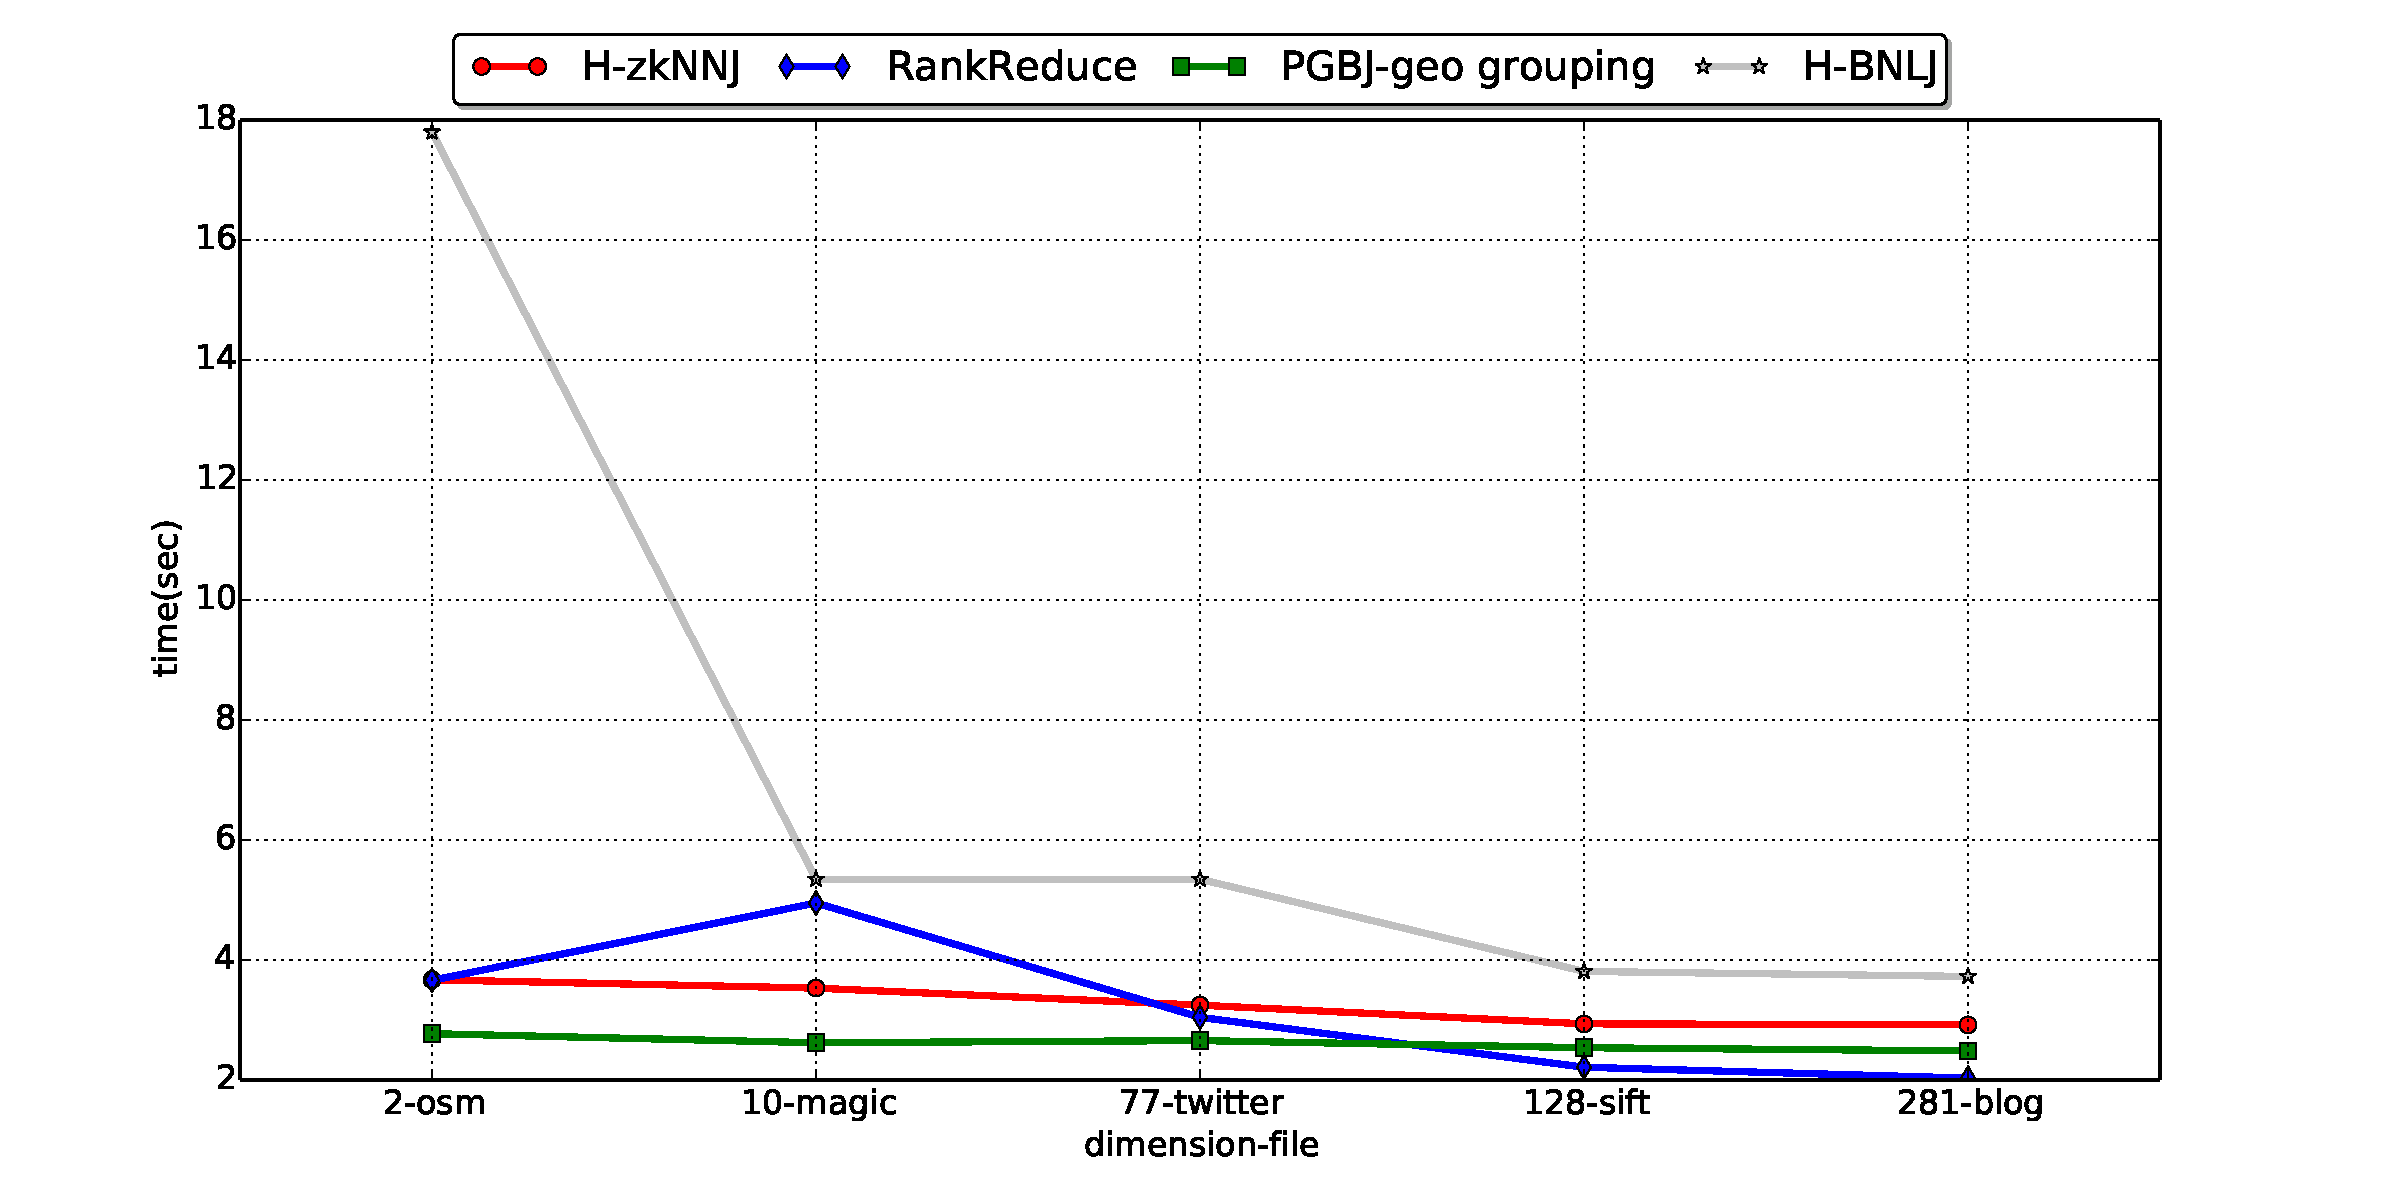
\includegraphics[width=1\textwidth]{img-perf/dim/datasettime.pdf} 
		\caption{Execution time% for real datasets of various dimensions%
		}
		\label{fig:dim_time}
	\end{subfigure}\begin{subfigure}[b]{0.5\textwidth}
	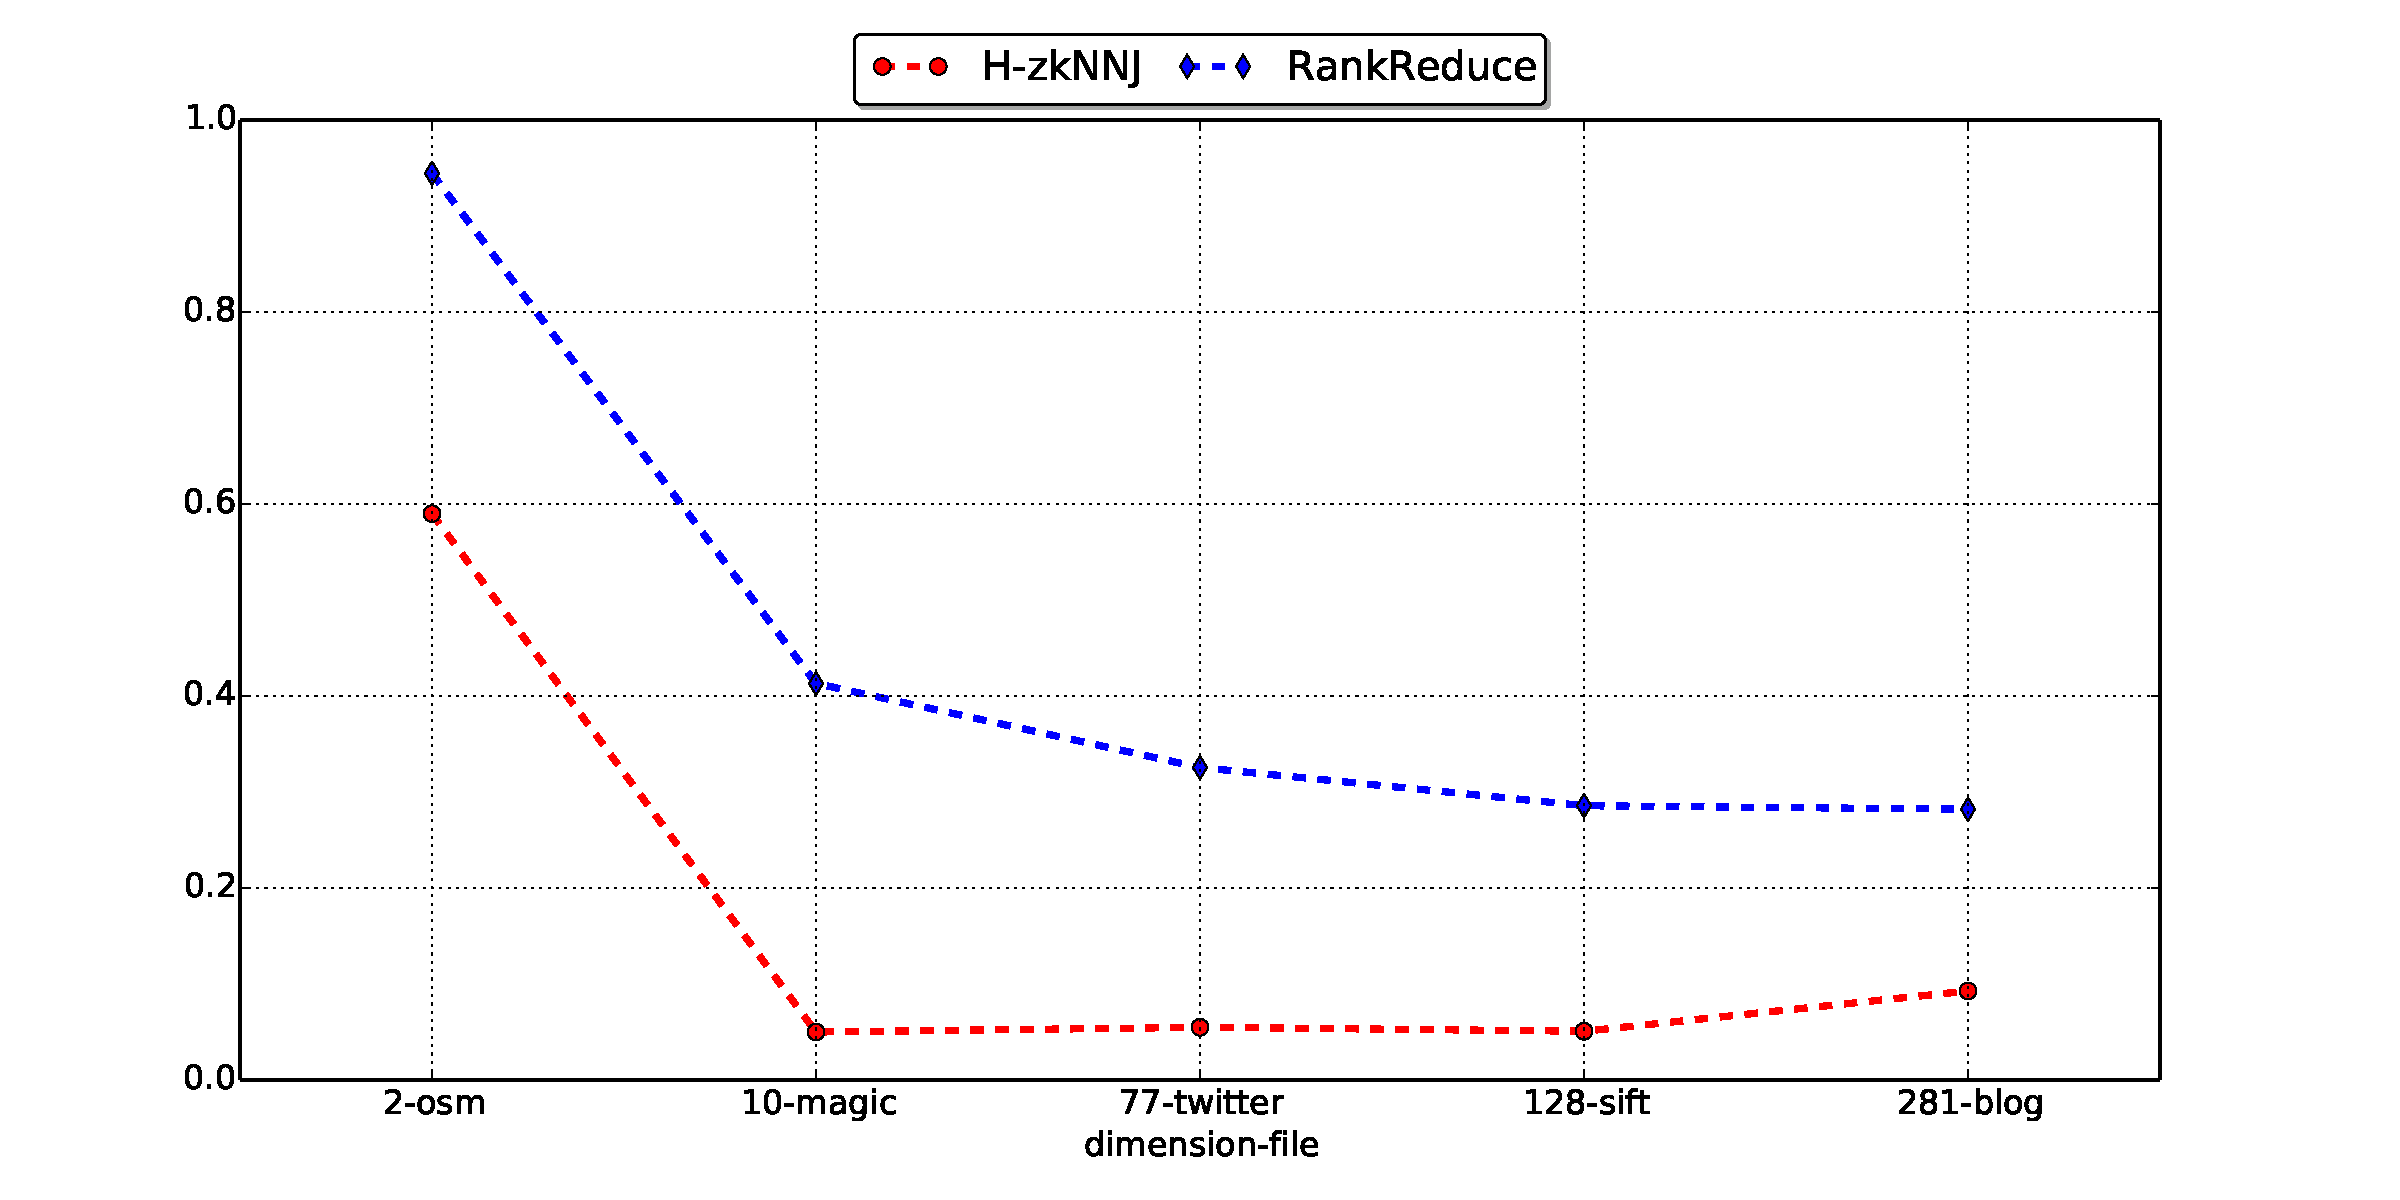
\includegraphics[width=1\textwidth]{img-perf/dim/datasetacc.pdf} 
	\caption{Recall and Precision %for real datasets of various dimensions%
	}
	\label{fig:dim_acc}
\end{subfigure}%
\caption{Real datasets of various dimensions}
\label{fig:dim_real}
\end{figure*} 

\begin{figure*}[ht]
	\centering
	\begin{subfigure}[b]{0.5\textwidth}
		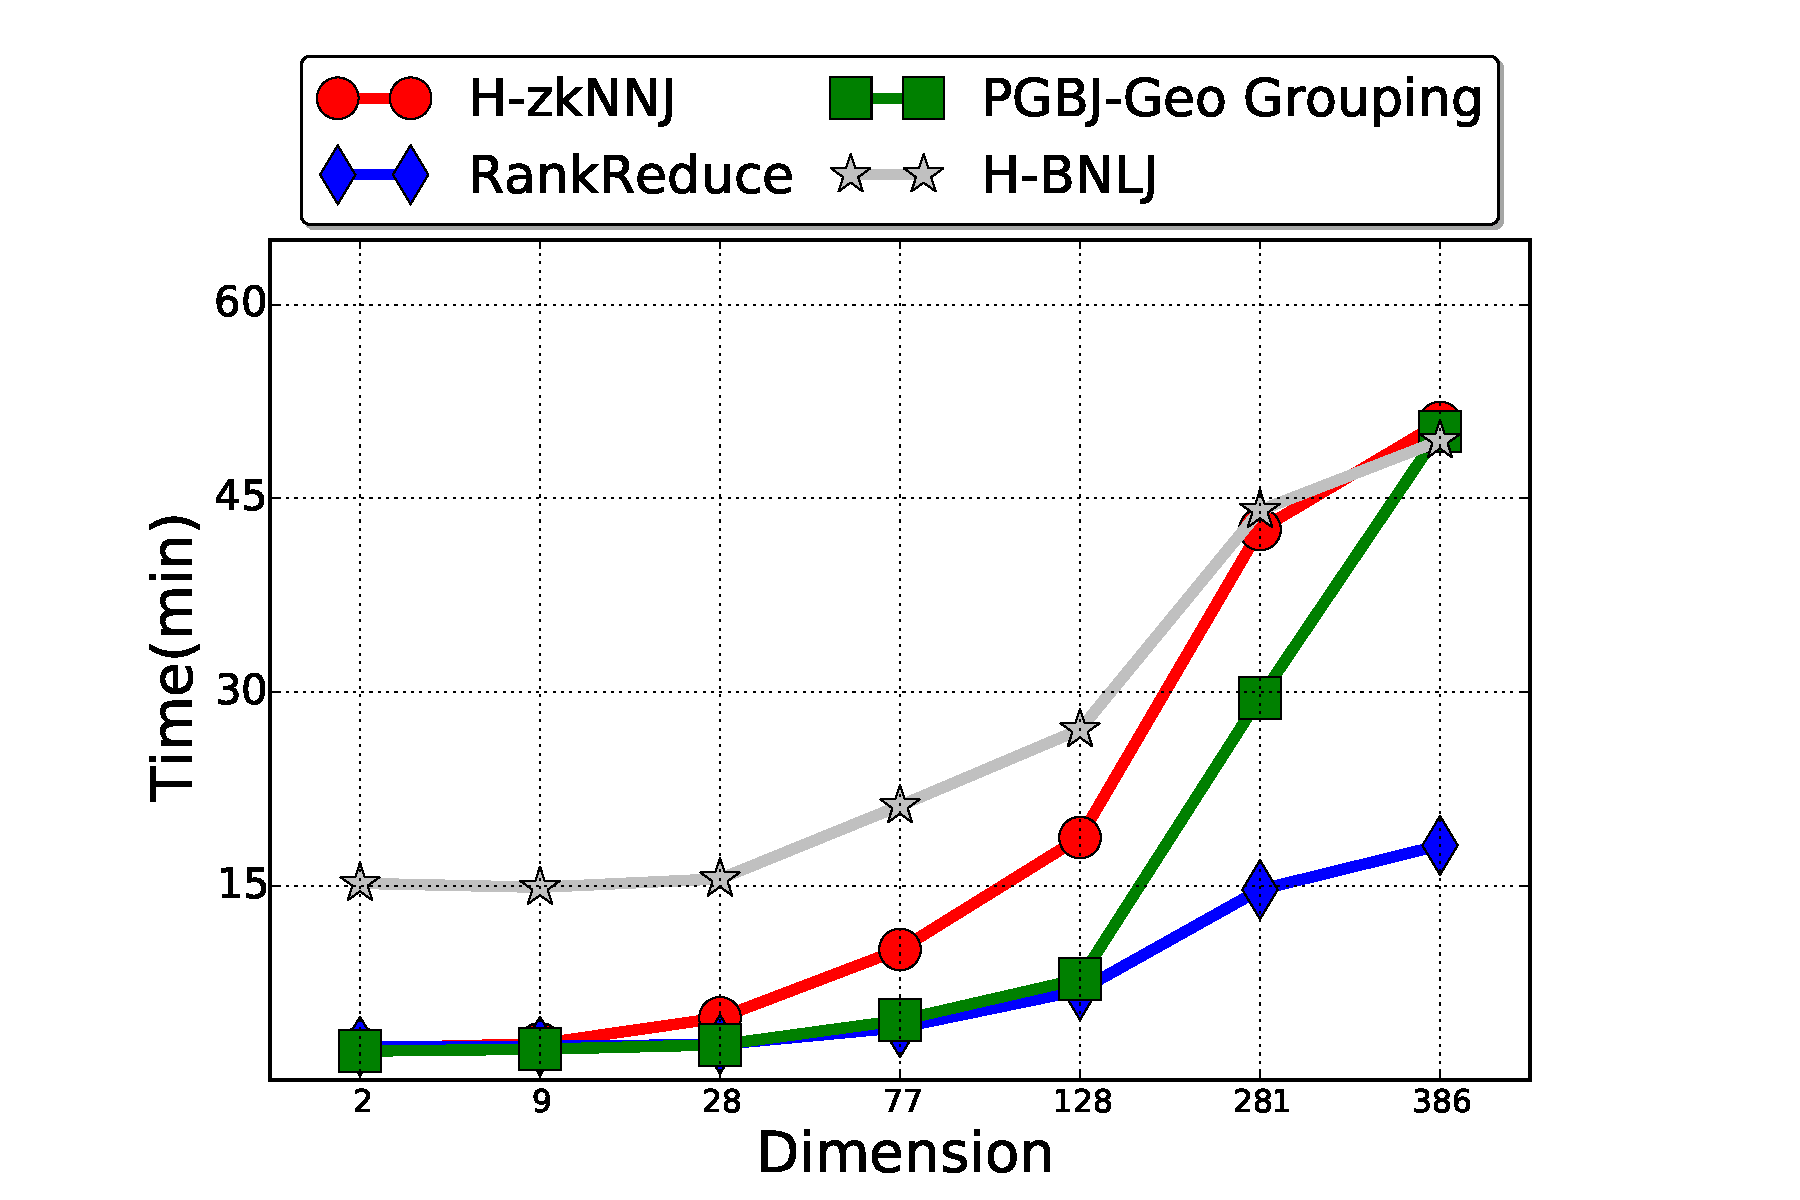
\includegraphics[width=1\textwidth]{img-perf/dim/randtime.pdf} 
		\caption{Execution time% for real datasets of various dimensions%
		}
		\label{fig:rand_time}
	\end{subfigure}\begin{subfigure}[b]{0.5\textwidth}
	
	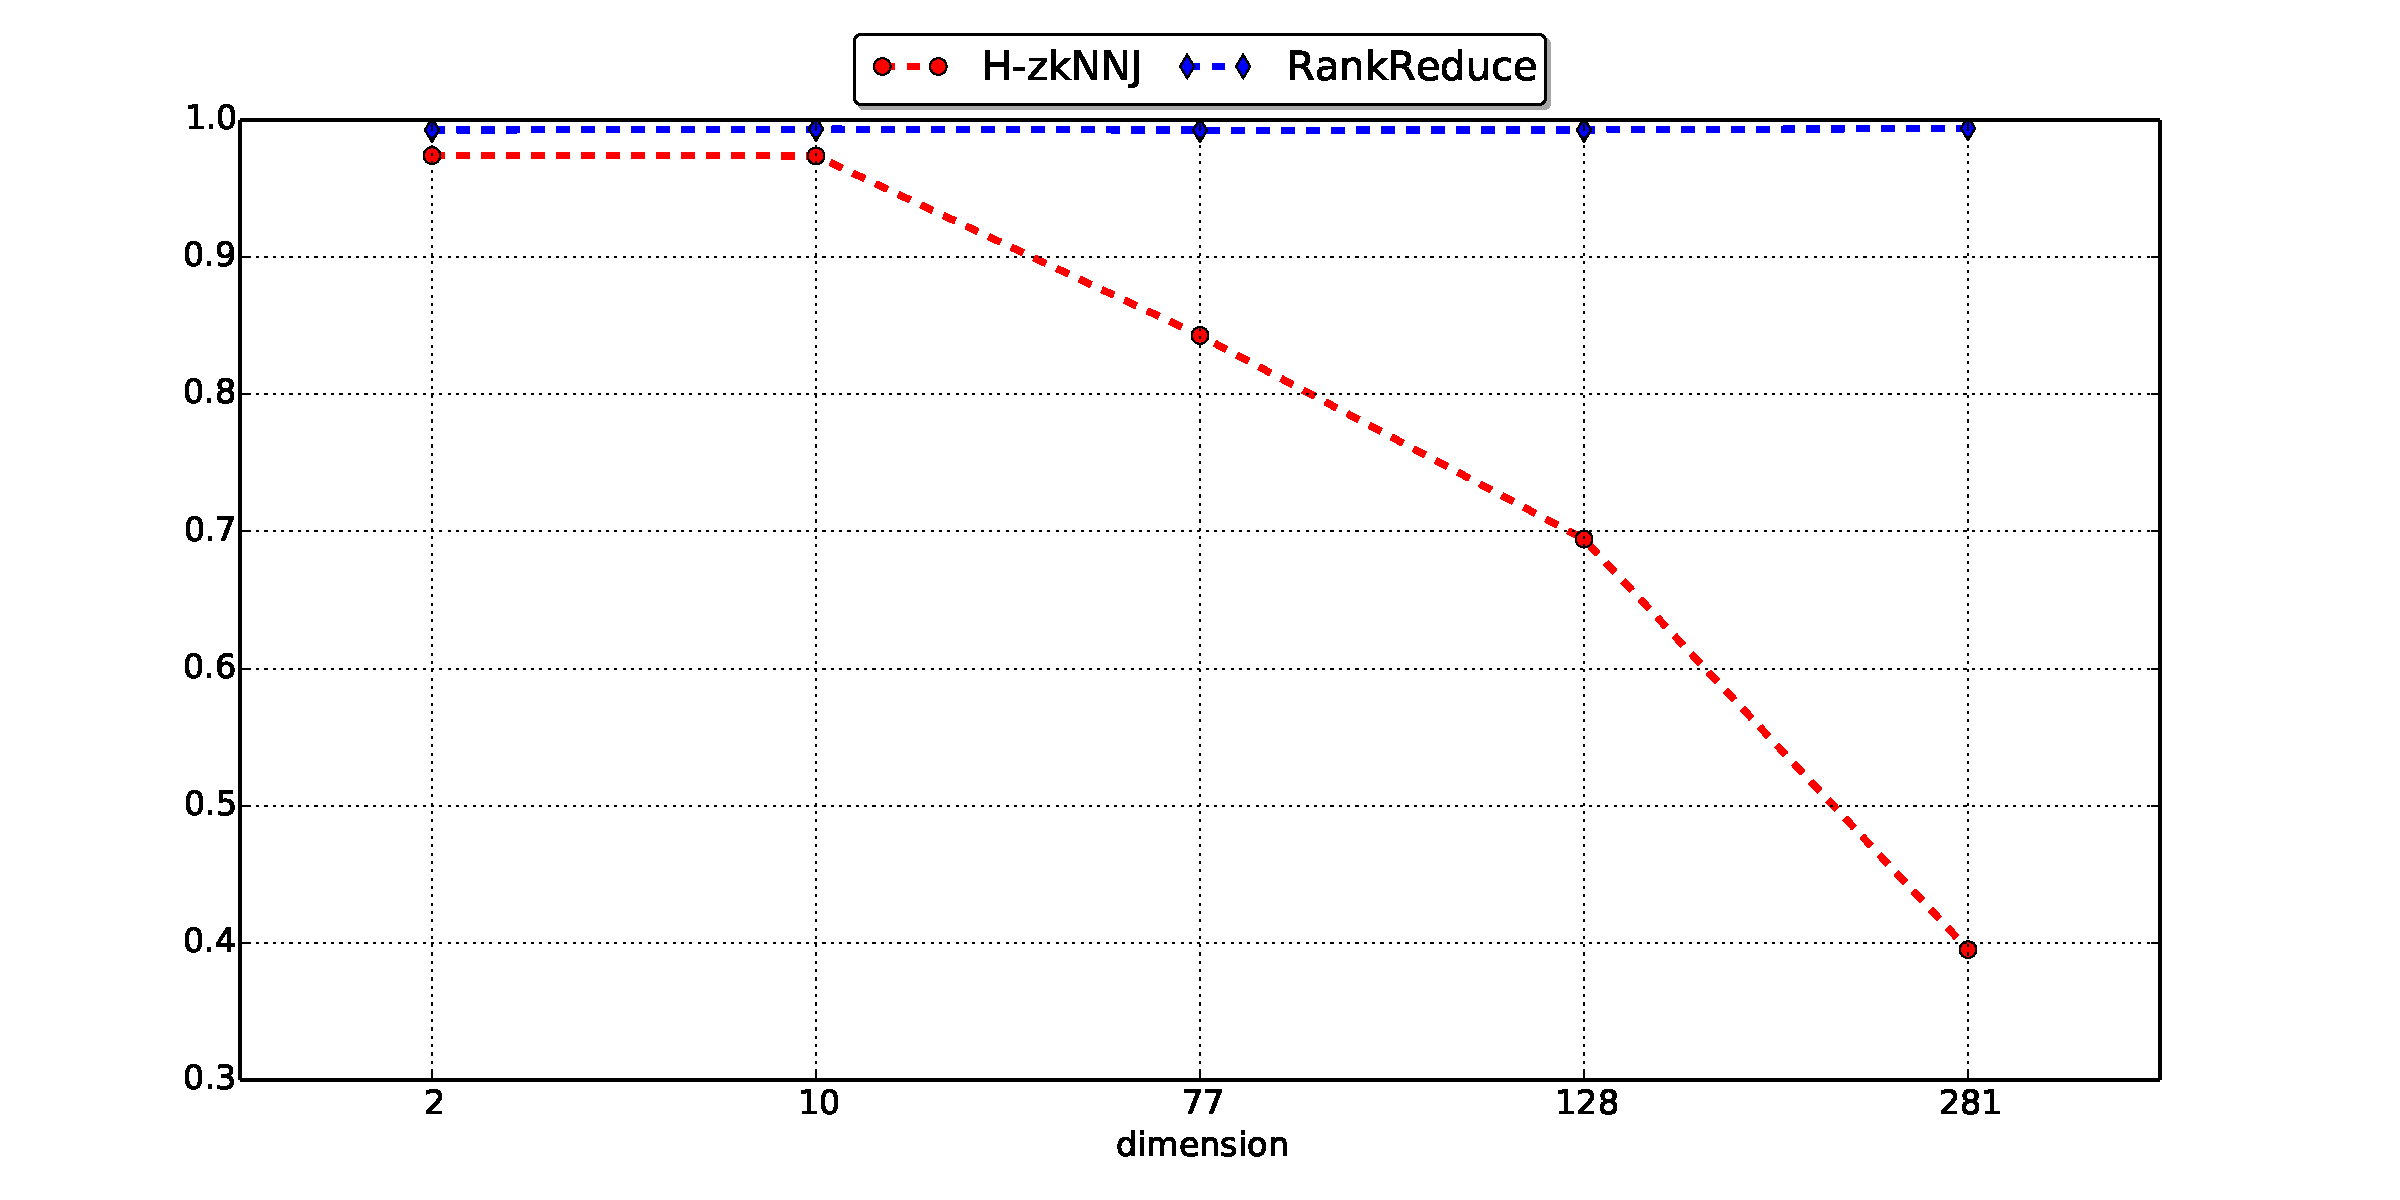
\includegraphics[width=1\textwidth]{img-perf/dim/randacc.pdf} 
	\caption{Recall and Precision}
	\label{fig:rand_acc}
\end{subfigure}%
\caption{Generated datasets of various dimensions}
\label{fig:dim_rand}
\end{figure*} 


Since \HBNLJ~relies on the dot product, it is not dataset dependent and its execution time increases
with the dimension as seen on Figures \ref{fig:dim_time} and \ref{fig:rand_time}. 

\VO~is heavily dependent on data distribution and on the choice of pivots to build clusters of 
equivalent size which improves parallelism. The comparison of execution times for the datasets 
\emph{128-sift} and \emph{281-blog} in Figure \ref{fig:dim_time} shows that, although the dimension
of data increases, the execution time is greatly reduced. Nonetheless, the clustering phase of the algorithm performs a 
lot of dot product operations which makes it dependent on the dimension, as can be seen in Figure \ref{fig:rand_time}. 

\Z~is an algorithm that depends on spatial dimension. Very efficient for low dimension, its 
execution time increases with the dimension (Figure \ref{fig:rand_time}). A closer 
analysis shows that all phases see their execution time increase. However, the overall time is 
dominated by the first phase (generation of shifted copies and partitioning) whose time complexity
sharply increases with dimension. Data distribution has 
an impact on the recall which gets much lower than the precision for some datasets (Figure~\ref{fig:dim_acc}).
With generated dataset (Figure~\ref{fig:rand_acc}), both recall and precision are identical and initially very high. 
However as dimension increases, the recall decreases because of the projection. 

Finally, \LSH~is both dependent on the dimension and distribution of data. Experiments with the real datasets have 
proved to be difficult because of the various parameters of the algorithm to obtain the requested number of 
neighbors without dramatically increasing the execution time (see discussion in Section~\ref{rankreduceanalysis}). 
Despite our efforts, the precision was very low for some datasets, in particular \emph{28-higgs}. 
Using the generated datasets, we see that its execution time increases with the dimension (Figure~\ref{fig:rand_time}) 
but its recall remains stable (Figure~\ref{fig:rand_acc}). 

\subsection{Practical Analysis}
In this section, we analyze the algorithms from a practical point of view, outlying their sensitivity to 
the dataset, the environment or some internal parameters.   
\subsubsection{H-BkNNJ}
%HBKNNJ
The main drawback of \HBK~is that only the Map phase is in parallel. In addition, the optimal parallelization 
is subtle to achieve because the optimal number of nodes to use is defined by  
$\frac{input\,size}{input\,split\,size}$. This algorithm is clearly not suitable for large datasets but because of its 
simplicity, it can, nonetheless, be used when the amount of data is small.  

\subsubsection{H-BNLJ}
In \HBNLJ, both the Map and Reduce phases are in parallel, but the optimal number of tasks is difficult to 
find. Given a number of partitions $n$, there will be $n^2$ tasks. Intuitively, one would choose a number of 
tasks that is a multiple of the number of processing 
units. The issue with this strategy is that the distribution of the partitions might be unbalanced.
Figure~\ref{fig:lb_hbnlj}
shows an experiment with $6$ partitions and $6^2=36$ tasks, each executed on a reducer. Some reducers will have more elements to process than others, 
slowing the computation.
\begin{figure}[!h]
\centering
   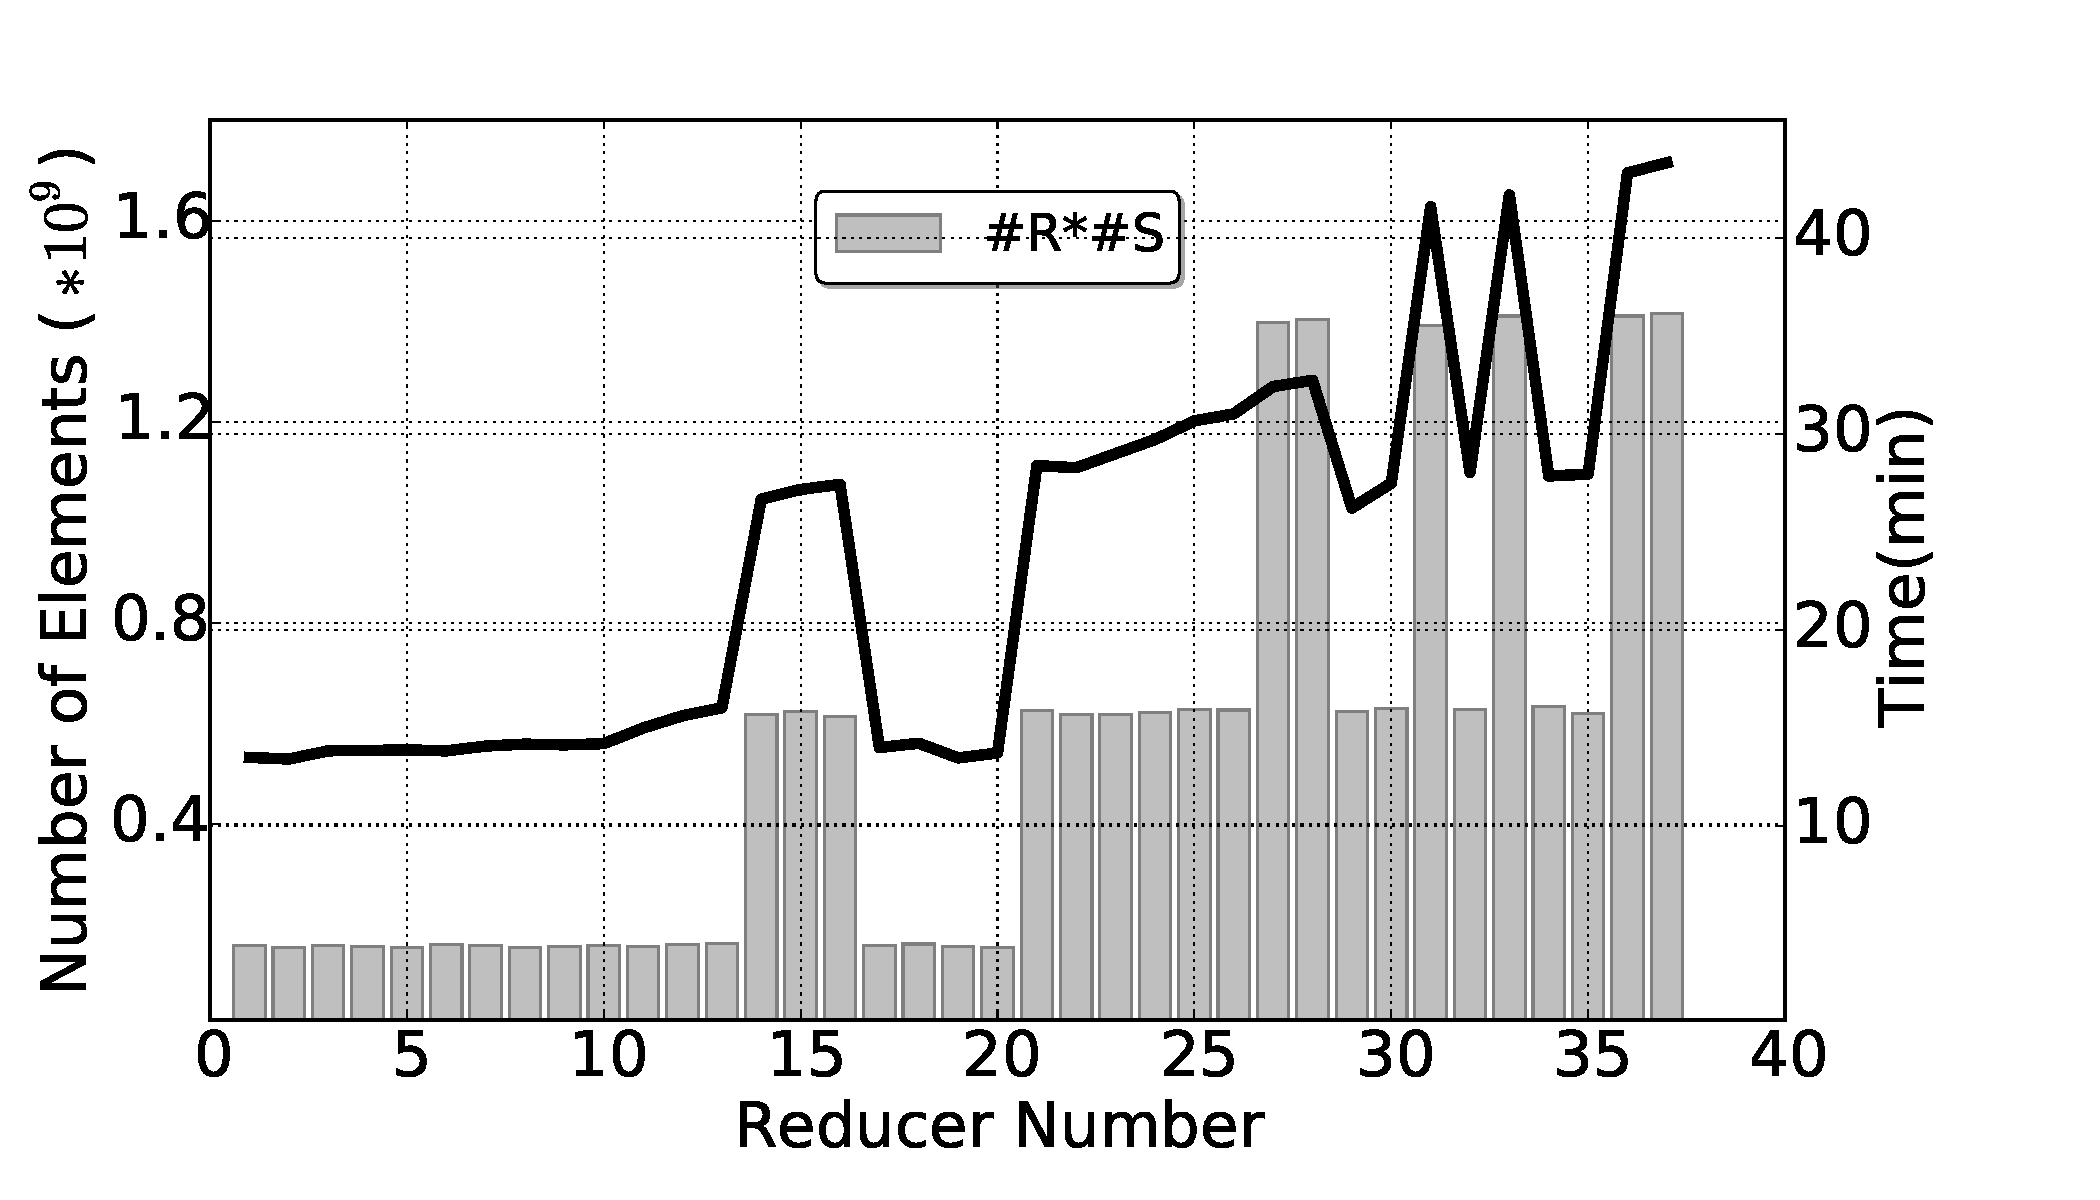
\includegraphics[width=0.4\textwidth]{img-perf/perso/loadbalancing/hbnlj.pdf}
   \caption{H-BNLJ, candidates job, $10^{5}$ records \label{fig:lb_hbnlj}, 6 partitions, Geo dataset}
\end{figure}%

Overall, the challenge with this algorithm is to find the optimal number of partitions for a given dataset. 

\subsubsection{PGBJ} 
A difficulty in \VO~comes from its sampling-based preprocessing techniques because it 
impacts the partitioning and thus the load balancing. This raises many challenges. First, how to choose
the pivots from the initial dataset. The three techniques proposed by the authors, farthest, k-means and 
random, lead to different pivots and different partitions and possibly different executions. We found that 
with  our datasets, both k-means and random techniques
gave the best performance. Second, the number of pivots is also important because
it will impact the number of partitions. A too small or too large number of pivots 
will decrease performance. Finally, another important parameter is the grouping strategy used 
(Section~\ref{pgbj_grouping}).
\begin{figure}[!h]
   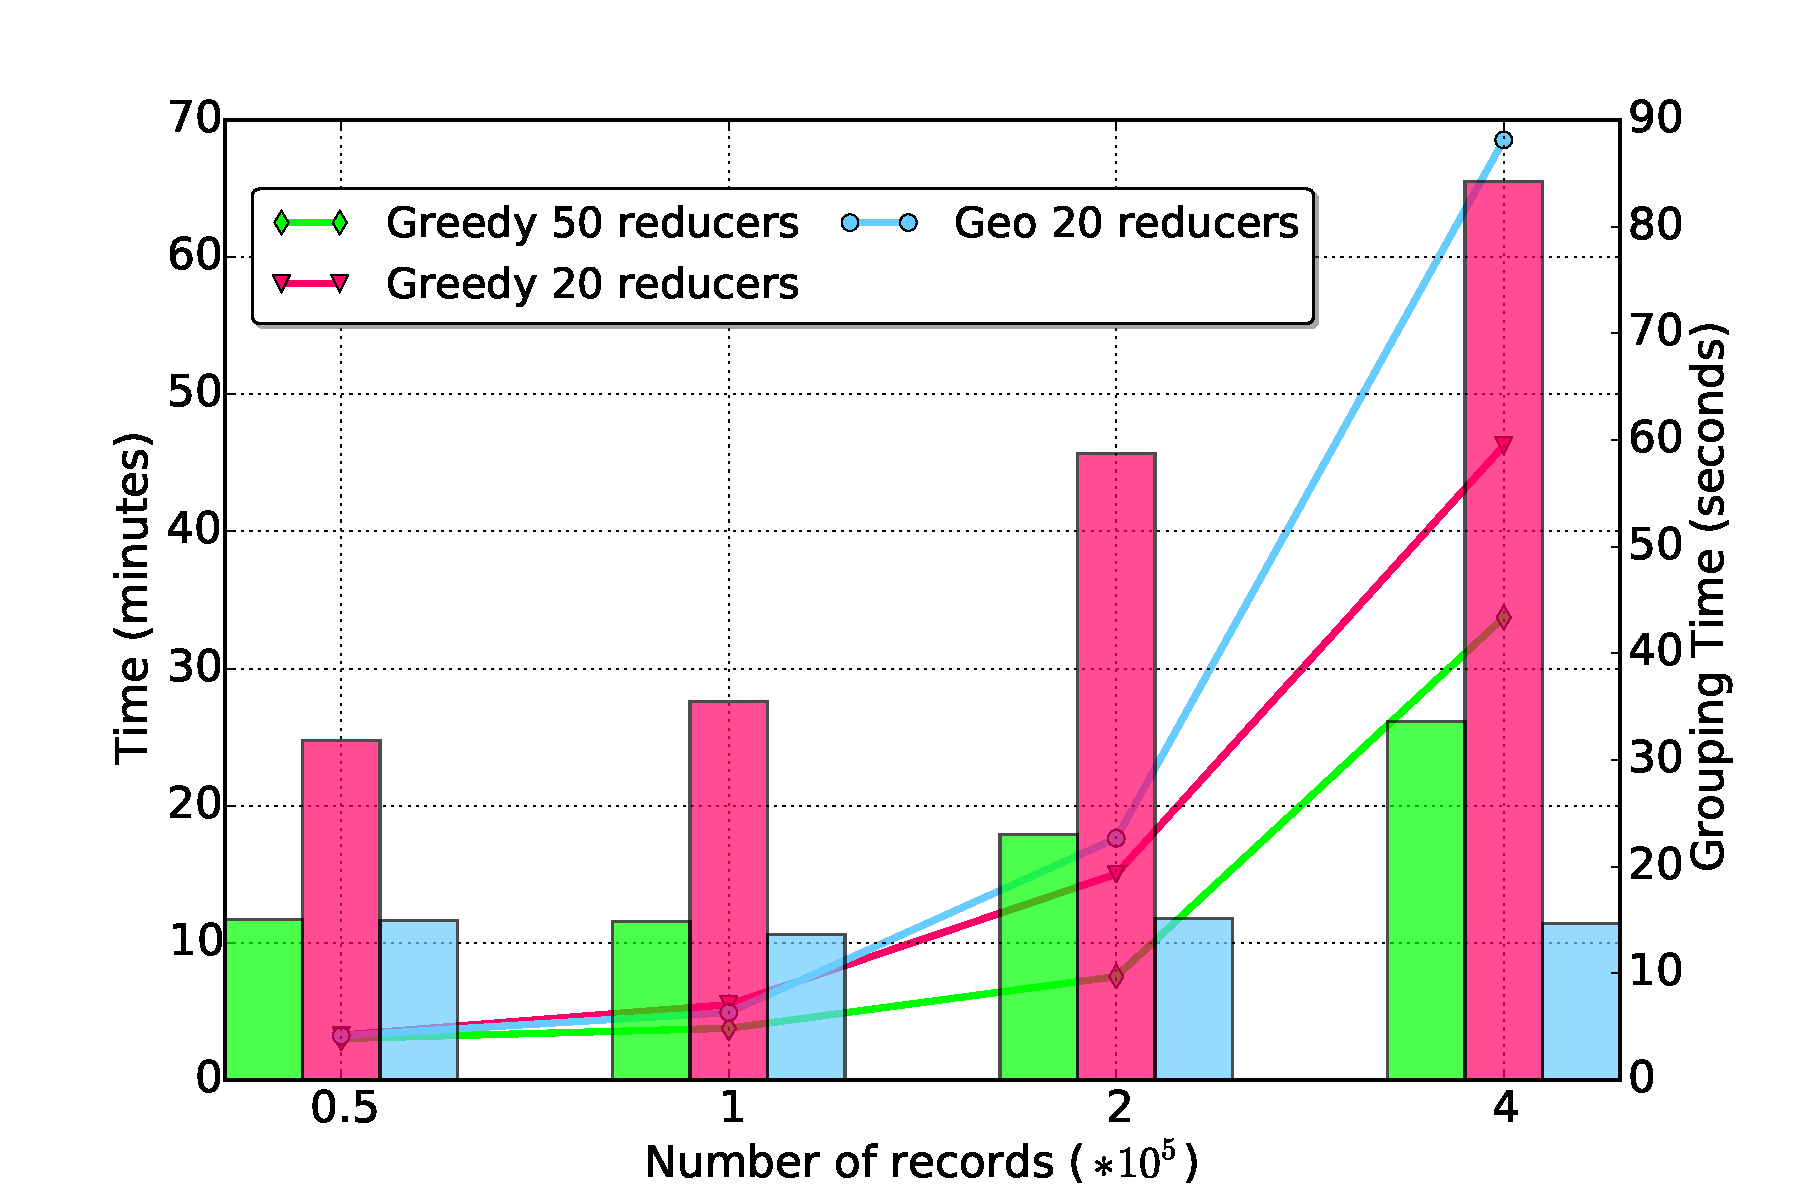
\includegraphics[width=0.5\textwidth]{img-perf/perso/pgbj/strategy.pdf} 
   \caption{PGBJ, overall time (lines) and Grouping time (bars)\label{fig:pgbj_strategy} with Geo dataset, 3000 pivots, 
   KMeans Sampling}         
\end{figure}
In Figure~\ref{fig:pgbj_strategy}, we can see that the greedy grouping technique has a higher grouping time 
(bars) than the geo grouping technique. 
However, the global computing time (line) using this technique is shorter thanks to the good load balancing. This
is illustrated by Figure~\ref{fig:pgbj_balancing} which shows the distribution of elements processed
by reducers when using geo grouping (\ref{fig:geo_20r}) or greedy grouping (\ref{fig:greedy_20r}).
                  
\begin{figure}[h]
\centering
		\begin{subfigure}[b]{0.25\textwidth}
                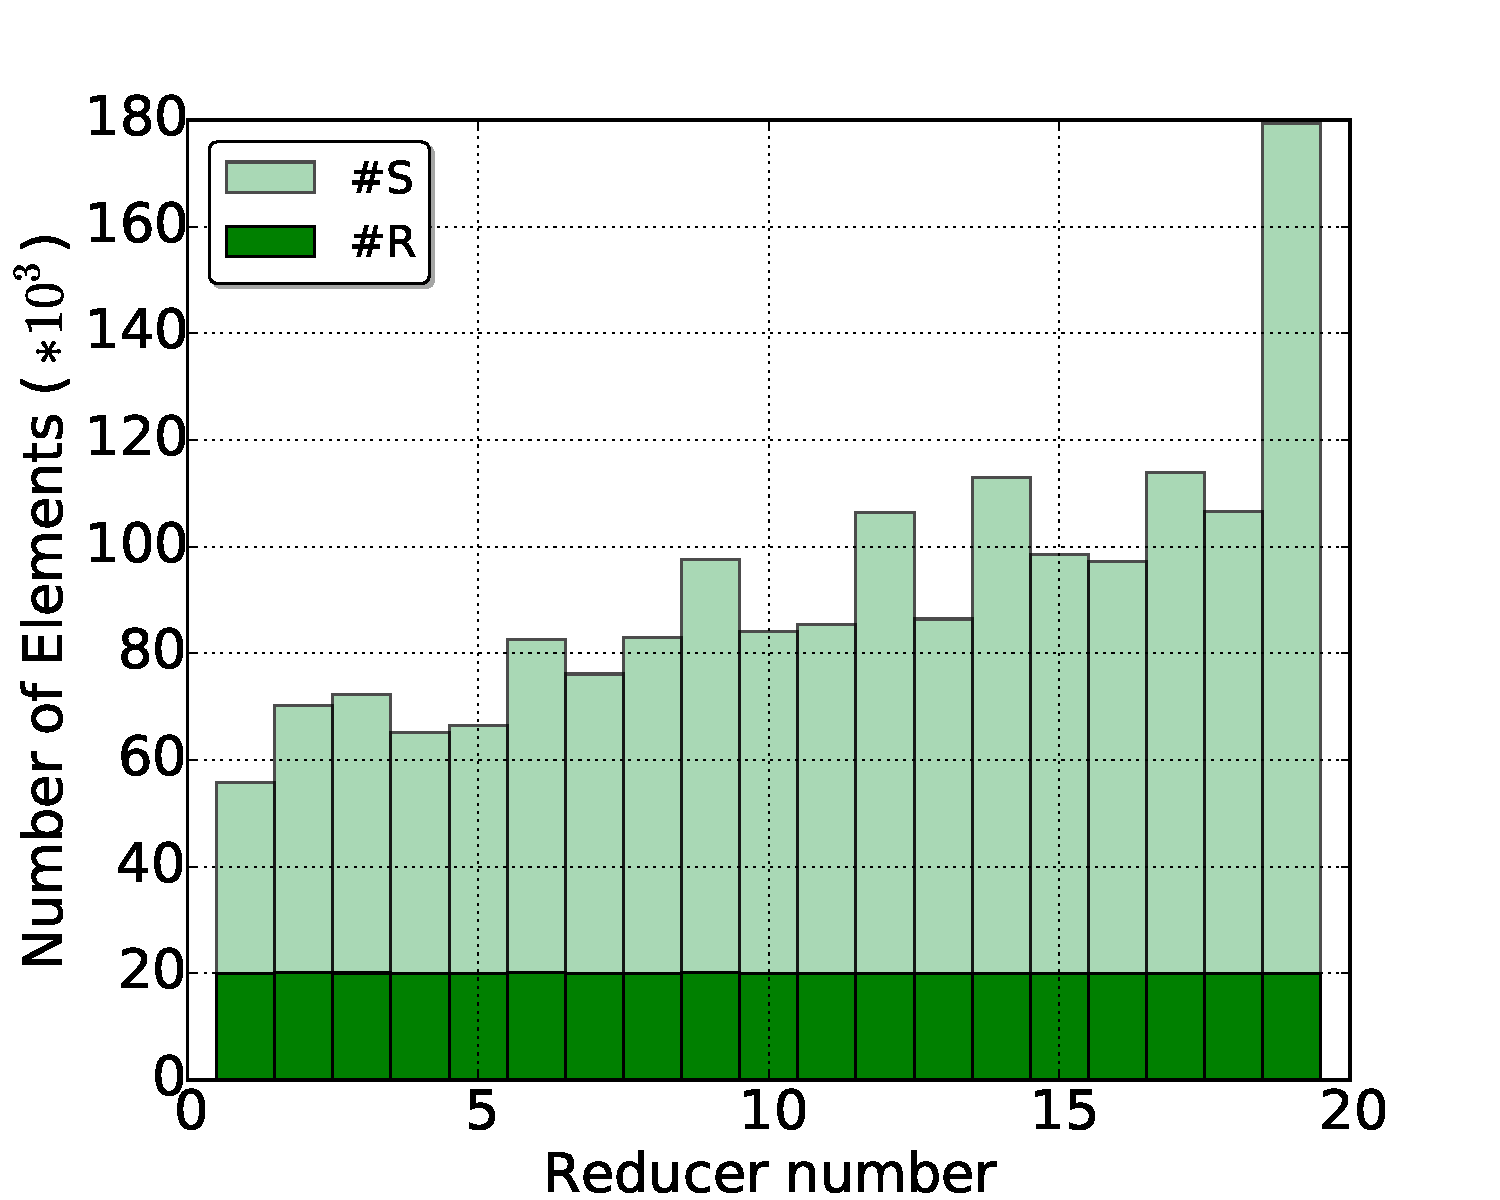
\includegraphics[width=\textwidth]{img-perf/perso/pgbj/geo_20r_400.pdf}
                \caption{Geo\label{fig:geo_20r}}
                
        \end{subfigure}%
        \begin{subfigure}[b]{0.25\textwidth}
                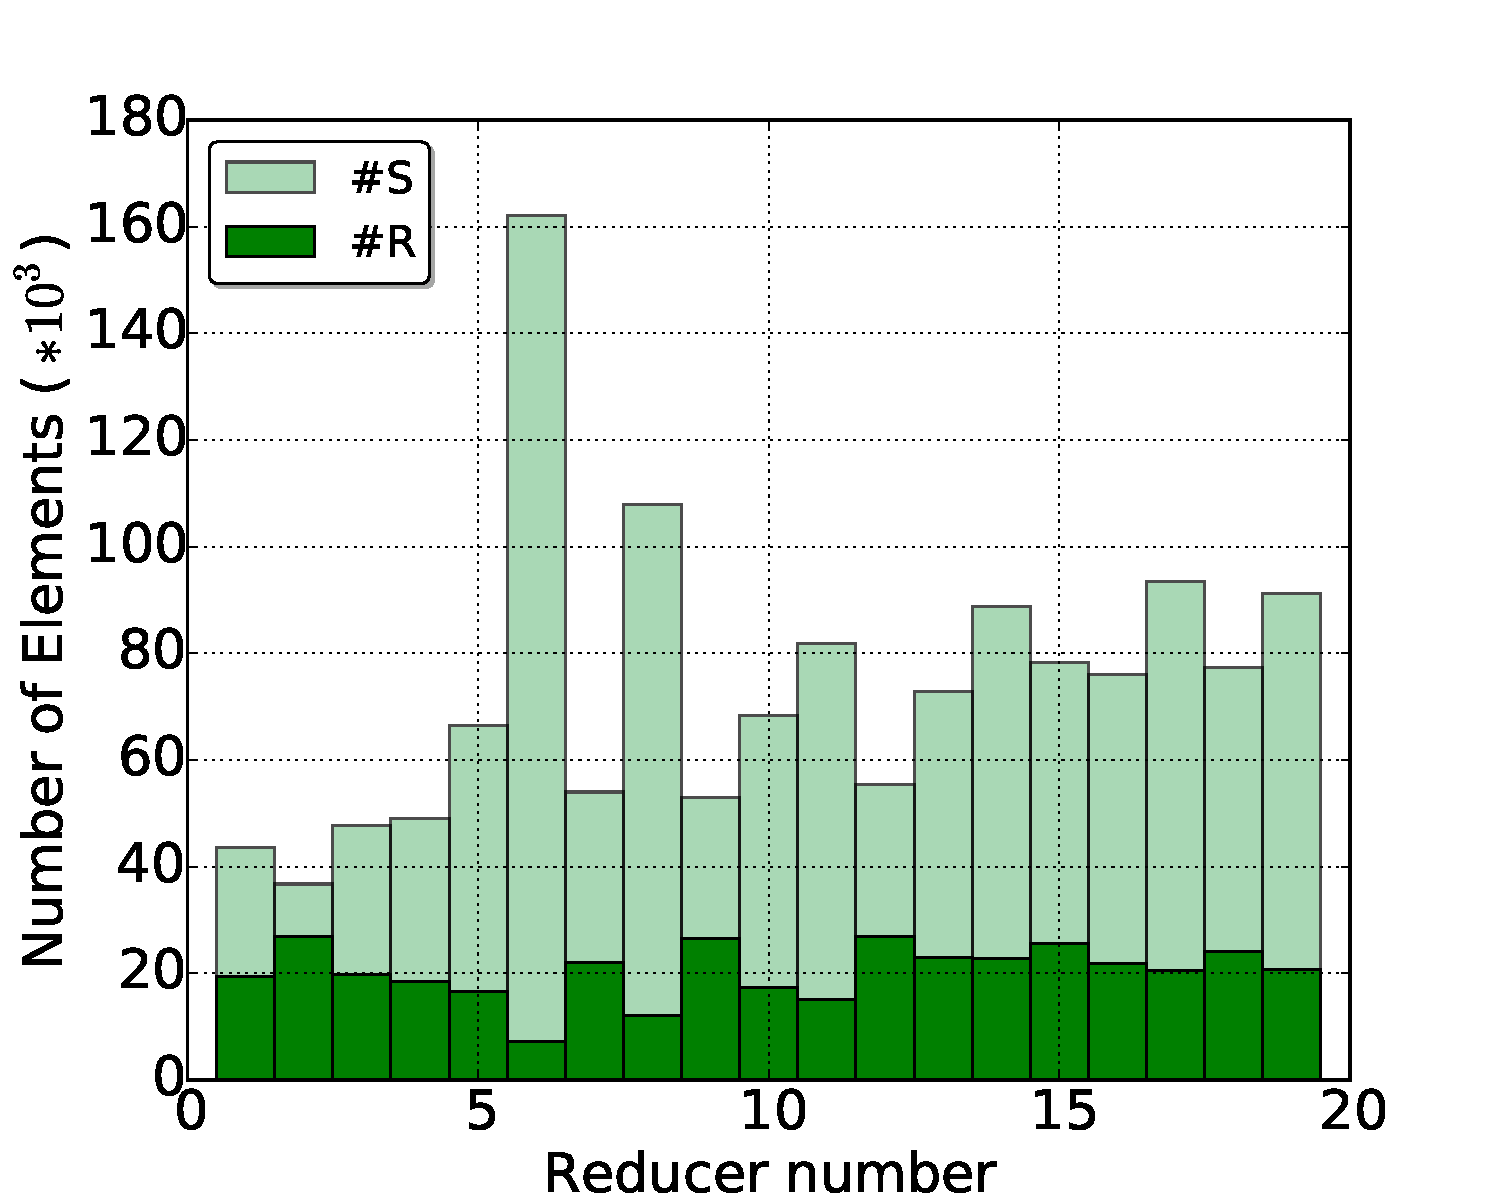
\includegraphics[width=\textwidth]{img-perf/perso/pgbj/greedy_20r_400.pdf}
                \caption{Greedy\label{fig:greedy_20r}}
                
        \end{subfigure}%
        \caption{PGBJ, load balancing \label{fig:pgbj_balancing} with 20 reducers}
\end{figure}                
 
\subsubsection{H-zkNNJ}\label{z-value}
In \Z, the $z$-value transformation leads to information loss. The recall of this algorithm is influenced
by  the nature, the dimension and the size of the input data.
More specifically, this algorithm becomes biased if the distance between initial data is very scattered, and 
the more input data or the higher the dimension, the more difficult it is to draw the space filling curve. To 
improve the recall, the authors propose to create duplicates in the original dataset by shifting data. 
This greatly increases the amount of data to process and has a significant impact on the execution time.

\begin{table*}[ht]
 	\begin{center}\renewcommand{\arraystretch}{1.2}
 		\begin{tabular}{|c|c|c|c|}
 			\hline
 			\textbf{Algorithm}  & \textbf{Advantage}  &  \textbf{Shortcoming}   & \textbf{Typical Usecase} \\
 			 \hline
 			\textbf{H-BkNNJ} 	& 
 				\begin{tabular}[c]{@{}c@{}}
 					Trivial to implement  
 				\end{tabular} & 
 				\begin{tabular}[c]{@{}c@{}}
 					1. Breaks very quickly \\ 
 					2. Optimal parallelism difficult\\ 
 					to achieve a priori
 				\end{tabular} &
 				\begin{tabular}[c]{@{}c@{}}
 			    	Any tiny and low dimension dataset\\
 			    	($\sim$ 25000 records)
 			    \end{tabular} \\ \hline
 			\textbf{H-BNLJ}     &
 				\begin{tabular}[c]{@{}c@{}}
 				 	Easy to implement
 				\end{tabular} & 
 				\begin{tabular}[c]{@{}c@{}}
 				 	1. Slow\\
 				 	2. Very large communication overhead 
 				\end{tabular} & 
 				\begin{tabular}[c]{@{}c@{}}
 				 	Any small/medium dataset\\
 				 	($\sim$ 100000 records)
 				\end{tabular} \\ \hline
 			\textbf{PGBJ}       & 
	 			\begin{tabular}[c]{@{}c@{}}
 				   	1. Exact solution\\ 
 				   	2. Lowest disk usage\\ 
 			       	3. No impact on communication\\
 			       	overhead with the increase of $k$
	 			\end{tabular}        & 
	 			\begin{tabular}[c]{@{}c@{}}
	 				1. Cannot finish in reasonable time\\ 
	 				for large dataset\\ 
	 				2. Poor performance for high\\
	 				dimension data\\
	 				3. Large communication overhead\\
	 				4. Performance highly depends on\\ 
	 				the quality of a priori chosen pivots
	 			\end{tabular} & 
 				\begin{tabular}[c]{@{}c@{}}
 					1. Medium/large dataset for\\
 					low/medium dimension\\
 					2. Exact results
 				\end{tabular} \\ \hline
 			\textbf{H-zkNNJ}    &
	 			\begin{tabular}[c]{@{}c@{}}
	 			    1. Fast\\ 
	 			    2. Does not require a priori parameter\\ 
	 			    tuning \\ 
	 			    3. More precise for large k \\ 
	 			    4. Always give the right number of $k$	 	
	 	        \end{tabular} & 
	 	        \begin{tabular}[c]{@{}c@{}}
	 	        	1. High disk usage\\ 
	 	        	2. Slow for large dimension \\ 
	 	        	3. Very high space requirement ratio \\ 
	 	        	for small values of $k$
 				\end{tabular} & 
 				\begin{tabular}[c]{@{}c@{}}
 					1. Large dataset of small dimension\\
 					2. High values of $k$\\
 			        3. Approximate results
 				\end{tabular} \\ \hline
 			\textbf{RankReduce} & 
 			\begin{tabular}[c]{@{}c@{}}
 				1. Fast\\ 
 				2. Low footprint on disk usage
 			\end{tabular} & 
 			\begin{tabular}[c]{@{}c@{}}
 				1. Fine parameter tuning required with\\ 
 				experimental set up \\
 				2. Multiple hash functions needed for\\
 				acceptable recall \\
 				3. Different quality metrics to consider\\
 				(recall + precision)
 		   \end{tabular}                                           
 			& \begin{tabular}[c]{@{}c@{}}
 				1. Large dataset of any dimension \\
 				2. Approximate results \\
 				3. Room for parameter tuning
 			\end{tabular} \\ \hline
 		\end{tabular}
 		\caption{Summary table for each algorithm in practice}\label{summary_practice}  
 	\end{center}
 \end{table*}

\subsubsection{RankReduce}\label{rankreduceanalysis}
\LSH, with the addition of a third job, can have the best performance of all, provided that it is started with the 
optimal parameters.
The most important ones are $W$, the size of each bucket, $L$, the number of hash families and $M$, the number 
of hash functions in each family. Since they are dependent on the dataset, experiments are 
needed to precisely tune them. In \cite{Dong:2008:MLP:1458082.1458172_full}, the authors suggests this can be achieved 
with a sample dataset and a theoretical model. 
The first important metric to consider is the number of candidates available in each bucket. Indeed, with some 
poorly chosen parameter values, it is possible to have less than $k$ elements in each bucket, making it impossible to 
have enough elements at the end of the computation (there are less than $k$ neighbors in the result). On the opposite, 
having too many candidates in each bucket will increase too much the execution time. 
To illustrate the complexity of the parameter tuning operation, we have run experiments on the Geo and SURF datasets. 
First, Figure~\ref{fig:lsh_tunning_geo} shows that, for the Geo dataset, increasing $W$ improves the recall and the 
precision at the expense of the execution time, up to an optimal before decreasing. This can be explained by looking
at the number of buckets for a given $W$. As $W$ increases, each bucket contains more elements and thus their number 
decreases. As a consequence, the probability to have the correct $k$ neighbors inside a bucket increases, which 
improves the recall. However, the computational load of each bucket also increases.

 
\begin{figure}[!h]
 \centering
          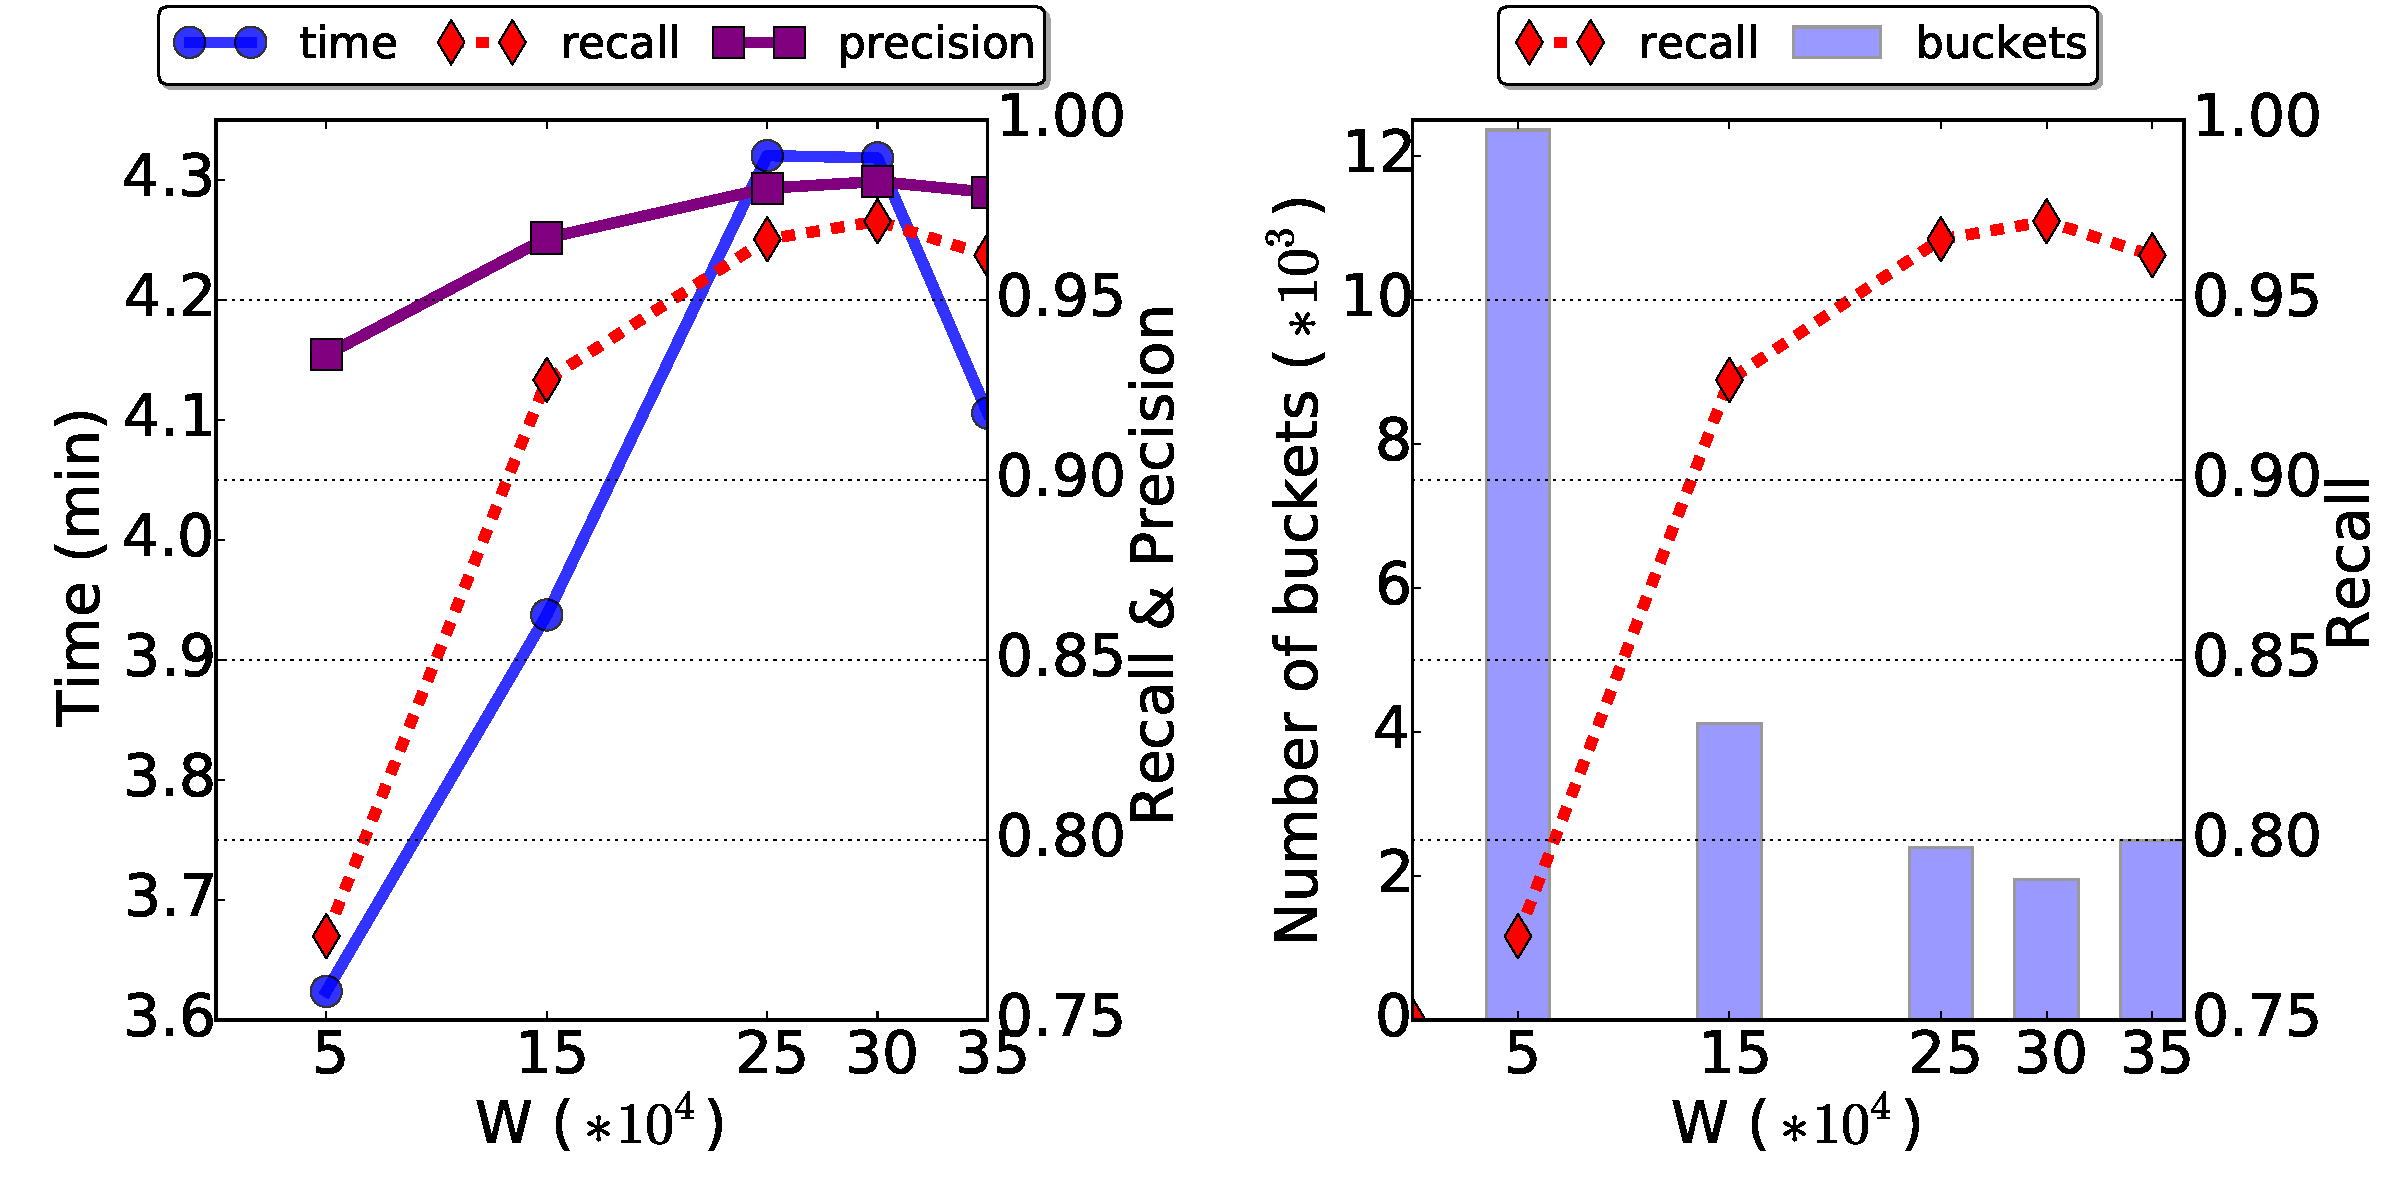
\includegraphics[width=0.5\textwidth]{img-perf/perso/lsh/params_geo_time.pdf} 
         \caption{LSH tuning, Geo dataset, 40k records,  20 nodes}
                \label{fig:lsh_tunning_geo}
\end{figure}
\begin{figure}[!h]
         \centering
       % \begin{subfigure}[b]{0.25\textwidth}
                 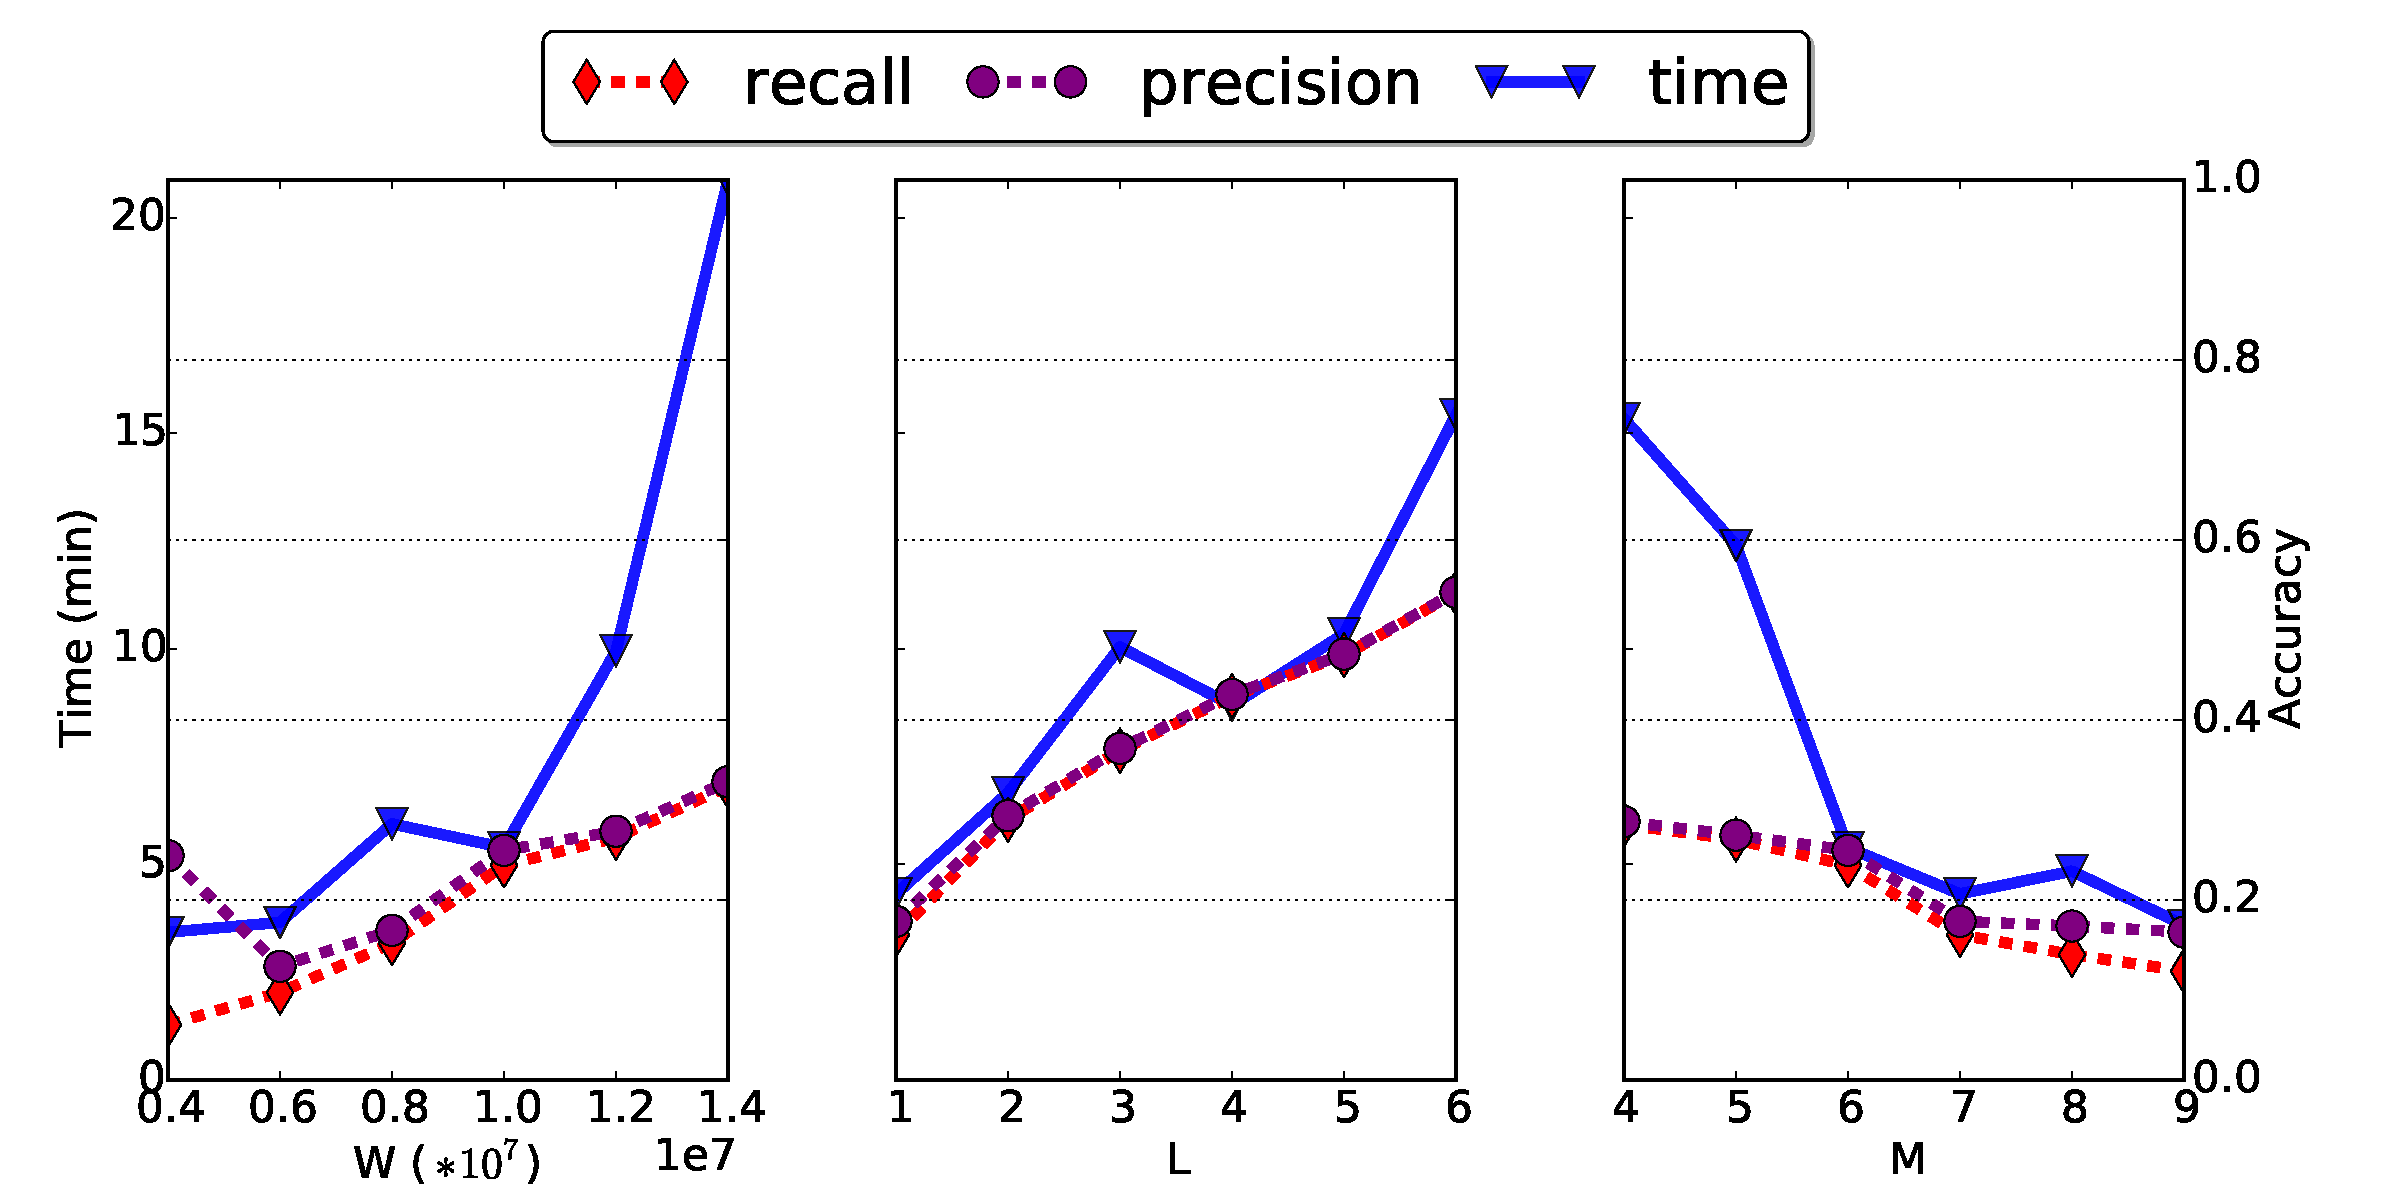
\includegraphics[width=0.5\textwidth]{img-perf/perso/lsh/params_surf.pdf} 
                %\caption{lsh tunning surf}
        %\end{subfigure}
         \caption{LSH tuning, SURF dataset, 40k records, 20 nodes}\label{fig:lsh_tunning_surf}
\end{figure}

A similar pattern can be observed with the SURF dataset (Figure~\ref{fig:lsh_tunning_surf}, left), where 
increasing $W$ improves the recall (from 5\% to 35\%) and the precision (from 22\% to 35\%). Increasing 
the number of families $L$ greatly improves both the precision and recall. However, increasing $M$, the
number of hash functions, decreases the number of collisions, reducing execution time but also the recall and 
precision. Overall, finding the optimal parameters for the LSH part is complex and has to be done for every dataset

After finishing all the experiments, we found that the execution time of all algorithms mostly follows the 
theoretical analysis presented in Section~\ref{sec:analysis}. However, as expected, the computationally intensive
part, which could not be expressed analytically, has proved to be very sensitive to a lot of different factors.
The dataset itself, through its dimension and the data distribution, but also the parameters of some of the 
pre-processing steps. The magnitude of this sensitivity and its impact on metrics such as recall and precision
could not have been inferred without thorough experiments. 


\subsection{Lessons Learned}

The first aspect is related to load balance. \HBNLJ~actually cannot guarantee load balancing, because of the random 
method it uses to split data. For \VO, Greedy grouping gives a better load balance than Geo grouping, at 
the cost of an increased duration of the grouping phase. At 
the same time, our experiments also confirm that \Z~and \LSH, which use size based 
partitioning strategies, have a very good load balance, with a very small deviation of the completion time of each 
task. %\TODO{3s out of how long? we need to put a \% ---done}

Regarding disk usage, generally speaking, \VO~has the lowest disk space requirement, while \Z~has the largest for small
$k$ values. However, for large $k$, the space requirement of all algorithms becomes similar. 
%\TODO{better word, comparable en francais}.

The communication overhead of \VO~is very sensitive to the choice of pivots. 

The data are another important aspect affecting the performance of the algorithms. As expected, all the 
algorithms' performance decreases as the dimension of data increases. However, what exceeded the prediction of the 
theoretical analysis is that the dimension is really a curse for \VO~. Because of the cost of computing distances in 
the pre-processing phase, its performance becomes really poor, sometimes worse than \HBNLJ. \Z~also suffers from the 
dimension, which decreases its recall. However, the major impact comes from the distribution of data. 

In addition, the overall performance is also sensitive to some specific parameters, especially for \LSH. Its 
performance depends a lot on some parameter tuning, which requires extensive experiments.

Based on the experimental results, we summarize the advantages, disadvantages and suitable usage scenarios for each 
algorithm, in Table~\ref{summary_practice}.


 

\section{Evaluation}\label{evaluation}
In order to compare theoretical performance and performance in practice, we performed an extensive experimental evaluation of the algorithms described in the 
previous sections.

The experiments were run on two clusters of Grid'5000\footnote{\url{www.grid5000.fr}}, one with Opteron 2218 processors 
and 8GB of memory, the other with Xeon E5520 processors and 32GB of memory, using Hadoop 1.3, 1Gb/s Ethernet and SATA hard drives. %\TODO{hard disk type, 
%ethernet. . Not useful, too much details}. 
We follow the default configuration of 
Hadoop: (1) the number of 
replications for each split of data is set 
to 3; (2) the number of slot of each node is 1, so only one map/reduce task is processed on the node at one time.
%\TODO{(3) the virtual memory for each map/reduce tasks is: xxx}

We evaluate the five approaches presented before.


 For \Z~and \HBNLJ, we took the source code provided by the authors as a starting 
point\footnote{\url{http://ww2.cs.fsu.edu/~czhang/knnjedbt/}} and added some modifications to reduce the size of 
intermediate files. The others were implemented from scratch using the 
description provided in their respective papers.

When implementing \LSH, we added a reduce phase to the first MapReduce job to compute some statistics information for 
each bucket. These information is used for achieving good load balance. %Using these statistics, a custom partitioner 
%distributes buckets among the 
%reducers to try to achieve good work balance. 
Moreover, in the original version, the authors only use one 
hash function. To improve the precision, we choose to use multiple families and hash functions depending on the 
dataset. Finally, our version of \LSH~ uses three MapReduce jobs instead of two.

Most of the experiments were ran using two different datasets: 

\begin{itemize}

\item \textbf{OpenStreetMap: }we call it the \emph{Geographic - or Geo - dataset}. The Geo dataset  
involves geographic XML data in two dimensions\footnote{Taken from: \url{http://www.geofabrik.de/data/download.html}}. 
This is a real dataset containing the location and description of objects. The data is organized by region. We extract 
$256*10^5$ records from the region of France.

\item \textbf{Catech 101: }we call it the \emph{Speeded Up Robust Features - or SURF - dataset}. It is a public set of images\footnote{Taken from: \url{www.vision.caltech.edu/Image_Datasets/Caltech101}}, which contains 101 categories of pictures of objects, and 40 to 800 images per category. 
SURF\cite{Surf} is a detector and a descriptor for points of interest in images, which produces image data
%Image feature descriptors are known to be high dimensional data, so we chose to use SURF\cite{Surf}, which produces image data
in 128 dimensions.  We extract 32 images per category, each image has between 1000 and 2000 descriptors.

\end{itemize}

In order to learn the impact of dimension and dataset, we use 5 additional datasets: \textbf{El Nino: } in 9 dimensions; \textbf{HIGGS: } in 28 dimensions; \textbf{TWITTER: } in 77 dimensions; \textbf{BlogFeedBack: } in 281 dimensions; and \textbf{Axial Axis: } in 386 dimensions. These data sets are all downloaded from UCI Machine Learning Repository\footnote{Taken from: \url{https://archive.ics.uci.edu/ml/}}.



We use a self-join for all our experiments, which means we use two datasets of equal sizes for $R$ and $S$ 
($|R|=|S|$). We also vary the number of 
records of each dataset from $0.125*10^5$ to $256*10^5$.
For all experiments, we have set $k=20$ unless specified otherwise. 
%The specified number of records is always the same for both $R$ and $S$ (query points and database points), i.e $|R|=|S|$ 
%although $R\cap S = \emptyset$ <- non au contraire R=S

We study the methods from the following aspects:
\begin{itemize}

\item The impact of data size

\item The impact of $k$

\item The impact of dimension and dataset

\end{itemize}

And we record the following information: the processing time, the disk space required, the recall and precision, and the communication overhead.

To assess the quality of the approximate algorithms, we compute two commonly used metrics and use the results of 
the exact algorithm \VO~as a reference. First, we define the recall as $ recall = \frac{\mid A(v) \bigcap I(v) 
\mid}{\mid  
I(v) \mid}$%\cite{Dong:2008:MLP:1458082.1458172_full}  
, where  $I(v)$ are the exact kNN of $v$ and $A(v)$ the kNN found 
by the approximate methods. Intuitively, the recall measures the ability of an algorithm to find the correct kNNs.
Another metric, the precision is defined by $precision =  \frac{\mid A(v) \bigcap I(v) \mid}{\mid  
A(v) \mid}$. It measures the fraction of correct kNN in the
final result set. By definition, the following properties holds: (1) $recall \leq precision$ because all the tested 
algorithms return up to $k$ elements. (2) if an approximate algorithms outputs $k$ elements, 
then  $ recall = precision$. 

Each algorithm produces intermediate data so we compute a metric called \emph{Space requirement} based on the size of
intermediate data ($Size_{intermediate}$), the size of the result ($Size_{final}$) and the size of the correct kNN 
($Size_{correct}$). We thus have $space = \frac{Size_{final}+Size_{intermediate}}{Size_{correct}}$.
% of possible kNN of $v$.
%Several parameters can impact the performance of computing kNN on MapReduce. We will focus on the size of the 
%input data in number of records for both $R$ and $S$, the number of machines used in the MapReduce cluster (thereafter 
%number of \emph{nodes}), the value of $k$ of the kNN query. 


We start by evaluating the most efficient number of machines to use (hereafter called \emph{nodes}) in terms of resources and computing 
time. For that, we measure the computing time of all algorithm for three different data input size of the geographic dataset.
The result can be seen on Figure \ref{fig:geo_data_nodes}.
\begin{figure}[!h]
 \centering
 %Fichier généré par excel/Nodes.xlsx 
 %Avec données datares/geo/nodes/
 %Fichier python perf/src/geo/timebyNodes.py
 \includegraphics[width=0.5\textwidth]{nodes.pdf}
 \caption{Impact of the number of nodes on computing time  \label{fig:geo_data_nodes}}
\end{figure}
As expected, the computing time is strongly related to the number of nodes. Adding more nodes increases parallelism, reducing the
overall computing time. There is however a significant slow down after using more than 15 machines. Based on those
results, and considering the fact that we later use larger datasets, we conducted all subsequent experiments using at 
most 20 nodes.


%\subsection{Geographic dataset}
\label{section:geo_dataset}

%%%% generated by 2-time.py
\begin{figure*}[htp]
	\centering
	\begin{subfigure}[b]{0.35\textwidth}
		\includegraphics[width=\textwidth]{img-perf/geo/data/time.pdf} 
		\caption{Time}
		\label{fig:geo_data_time}
	\end{subfigure}%
	\begin{subfigure}[b]{0.35\textwidth}
		\includegraphics[width=\textwidth]{img-perf/geo/data/memory.pdf} 
		\caption{Result size and Disk Usage}
		\label{fig:geo_data_memory}
	\end{subfigure}%
	\begin{subfigure}[b]{0.35\textwidth}
		\includegraphics[width=\textwidth]{img-perf/geo/data/accuracy.pdf} 
		\caption{Recall and Precision \label{fig:geo_data_acc}}
	\end{subfigure}%
	\caption{Geo dataset impact of the data set size \label{geo_dataset}}
\end{figure*}


For all experiments in this section, we used the parameters described in Table~\ref{table:parameters_geo}.
Details regarding each parameter can be found in sections \ref{data_preprocessing} and  \ref{partitioning}. For 
RankReduce, the value of $W$ was adapted to get the best performance from each dataset. For datasets up to $16*10^5$
records, $W=32*10^{5}$, up to $25*10^{5}$ records, $W=25*10^{5}$ and finally, $W=15*10^{5}$ for the rest of the 
experiments. 

% shown in Table~\ref{table:parameters_geo}.
\begin{table}[ht]
\begin{center}{\renewcommand{\arraystretch}{1.2} % to prevent equation from being chopped 
\begin{tabular}{|c|c|c|c|}
\hline
\textbf{Algorithm} & \textbf{Partitioning} & \textbf{Reducers} & \textbf{Configuration}  \\ \hline
\HBNLJ             & 10 partitions  & 100 reducers & \\ \hline
\VO               & 3000 pivots     & 25 reducers       & \begin{tabular}[c]{@{}c@{}}k-means \\ + greedy\end{tabular} 
\\ \hline
\LSH          & $W = \left\{
\begin{array}{l}  
	32*10^{5}\\    
    25*10^{5}\\
	15*10^{5}\\
\end{array}\right.$
%$32*10^{5}$
% \TODO{this is plustot the size of bucket but not the number of partition. ??}           
& 25 reducers       & \begin{tabular}[c]{@{}c@{}}L = 2\\ M = 7\end{tabular}       \\ \hline
\Z~           & 10 partitions         & 30 reducers       & 3 shifts, 
p=10                                                     \\ \hline
\end{tabular}
}
\caption{Algorithm parameters \label{table:parameters_geo} for geographic dataset}
\end{center}
\end{table}


\subsubsection{Impact of input data size}
Our first set of experiments measures the impact of the data size on execution time, disk space and recall. 
Figure~\ref{fig:geo_data_time} shows the global computing time of all algorithms, varying 
the number of records from $0.125 * 10^{5}$ to $256 * 10^{5}$. The global computing time increases more or less 
exponentially for all algorithms, but only \Z~and \LSH~can process medium to large datasets. For 
small datasets, \VO~can compute an exact solution as fast as the other algorithms. 


Figure~\ref{fig:geo_data_memory} shows the space requirement of each algorithm as a function of the final output size. 
To 
reduce the footprint of each run, intermediate data are compressed. For example, for 
\HBNLJ, the size of intermediate data is $2.6$ times bigger than the size of output data. Overall, the algorithms with 
the
lowest space requirements are \LSH~and \VO.

Figure~\ref{fig:geo_data_acc} shows the recall and precision of the two approximate algorithms, \Z~and \LSH. Since \Z~
always return $k$ elements, its precision and recall are identical. 
As the number of records increases, its recall decreases, while still being high, because of the 
space filling curves used in the preprocessing phase.
On the other hand, the recall of \LSH~is always lower than its precision because it outputs less than $k$ elements. It
benefits from larger datasets because more data end up in the same bucket, increasing the 
number of candidates. Overall, the quality of \LSH~was found to be better than \Z~on the Geo dataset. 

%\input{parts/exp-dim-figure.tex}
\subsubsection{Impact of k}
Changing the value of $k$ can have a significant impact on the performance of some of the kNN 
algorithms. We experimented on a dataset of $2*10^5$ records (only $5*10^4$ for \HBNLJ~ 
for performance reasons) with values for $k$ varying from 2 to 512. Results are shown in 
Figure~\ref{fig:geo_impact_k} using a logarithmic scale on the x-axis.

First, we observe a global increase in computing time (Figure~\ref{fig:geo_k_time}) which matches the complexity 
analysis performed earlier. 
As $k$ increases, the performance of \Z, compared to the other advanced algorithms, decreases. This is due to the 
necessary replication of the $z$-values of $S$ throughout the partitions to find enough candidates: the core 
computation is thus much more complex. 

%%% generated by A4-ratioByK.py
\begin{figure*}[htp]
	\centering
	\begin{subfigure}[b]{0.35\textwidth}
		\includegraphics[width=\textwidth]{img-perf/geo/k/time.pdf} 
		\caption{Time\label{fig:geo_k_time}}       
	\end{subfigure}%
	\begin{subfigure}[b]{0.35\textwidth}
		\includegraphics[width=\textwidth]{img-perf/geo/k/memory.pdf} 
		\caption{Result size and Disk Usage\label{fig:geo_k_memory} }
	\end{subfigure}%
	\begin{subfigure}[b]{0.35\textwidth}
		\includegraphics[width=\textwidth]{img-perf/geo/k/accuracy.pdf} 
		\caption{Recall and Precision \label{fig:geo_k_acc}}            
	\end{subfigure}%
	\caption{ Geo dataset with 200k records (50k for H-BNLJ), impact of $K$  }
	\label{fig:geo_impact_k}
\end{figure*}

Second, the algorithms can also be distinguished considering their disk usage, visible on 
Figure ~\ref{fig:geo_k_memory}. The global tendency is that the ratio of intermediate data size over the final data 
size decreases. This means that for each algorithm the final 
data size grows faster than the intermediate data size. As a consequence, there is no particular algorithm that 
suffers from such a bottleneck at this point.
\VO~is \ the most efficient from this aspect. Its replication of data occurs independently of the number of 
selected neighbors. Thus, increasing $k$ has a small impact on this algorithm, both in computing time and space 
requirements. On this figure, an interesting observation can also be made for \Z. For $k=2$, it has by far the 
largest disk
usage but becomes similar to the others for larger values. 
This is because \Z~creates a lot of intermediate data (copies of the initial dataset, vectors for the space 
filling curve, sampling...) irrespective of the value of $k$. As $k$ increases, so does the output size, mitigating the 
impact of these intermediate data. 

Surprisingly, changing $k$ has a different impact on the recall of the approximate kNN methods, as can be seen on 
Figure~\ref{fig:geo_k_acc}.
For \LSH, increasing $k$ has a negative impact on the recall which sharply decreases when $k\geq 64$. This is
because the window parameter ($W$) of LSH was set at the beginning of the experiments to achieve the best performance for this
particular dataset. However, it was not modified for various of $k$. Thus it became less optimal as $k$ increased. This 
shows there is a link between global parameters such 
as $k$ and parameters of the LSH process. When using \Z, 
increasing $k$  improves the precision: the probability to have incorrect points is reduced as there are more 
candidates in a single partition. 

\subsubsection{Communication Overhead}
Our last set of experiments looks at inter-node communication by measuring the amount of data transmitted during the
shuffle phase (Figure~\ref{fig:geo_communication}). The goal is to compare these measurements with the theoretical 
analysis in Section~\ref{section:global_complexity}, 

%%%% Generated with   2-time.py  and A4-ratioByK.py
\begin{figure*}[htp]
	\centering
	\begin{subfigure}[b]{0.48\textwidth}
		\includegraphics[width=\textwidth]{img-perf/geo/data/shuffle.pdf} 
		\caption{Impact of the data set size\label{fig:geo_data_shuffle}}
	\end{subfigure}%
	\begin{subfigure}[b]{0.48\textwidth}
		\includegraphics[width=\textwidth]{img-perf/geo/k/shuffle.pdf} 
		\caption{Impact of $K$ with $2*10^5$ records ($0.5*10^5$ for H-BNLJ) \label{fig:geo_k_shuffle}}
	\end{subfigure}%
	\caption{Geo dataset, communication overhead \label{fig:geo_communication}}      
\end{figure*}

\emph{Impact of data size.} For Geo dataset (Figure~\ref{fig:geo_data_shuffle}), \HBNLJ~has indeed a lot of 
communication. For a dataset of $1*10^5$ records, the shuffle phase transmits almost $4$ times the original size.
Both \LSH~and \Z~have a constant factor of $1$ because of the duplication of the original 
dataset
to improve the recall. The most efficient algorithm is \VO~for two reasons. First it does not duplicate the 
original dataset and second, it relies on various grouping strategies to minimize replication.

\emph{Impact of k.}
We have performed another set of experiments, with a fixed dataset of $2*10^5$ records (only $0.5*10^5$ for \HBNLJ). 
The results can be seen in Figure~\ref{fig:geo_k_shuffle}. For different values of $k$, we have a similar hierarchy 
than with the data size. For \LSH~and \Z, the shuffle increases linearly because the number of candidates in the second 
phase depends on $k$. Moreover \Z~also replicates $k$ previous and succeeding elements in the first phase, and because 
of that, its overhead becomes significant for large $k$. Finally in \VO, $k$ has no impact on the shuffle phase.

\subsection{Geographic dataset}
\label{section:geo_dataset}

%%%% generated by 2-time.py
\begin{figure*}[htp]
	\centering
	\begin{subfigure}[b]{0.35\textwidth}
		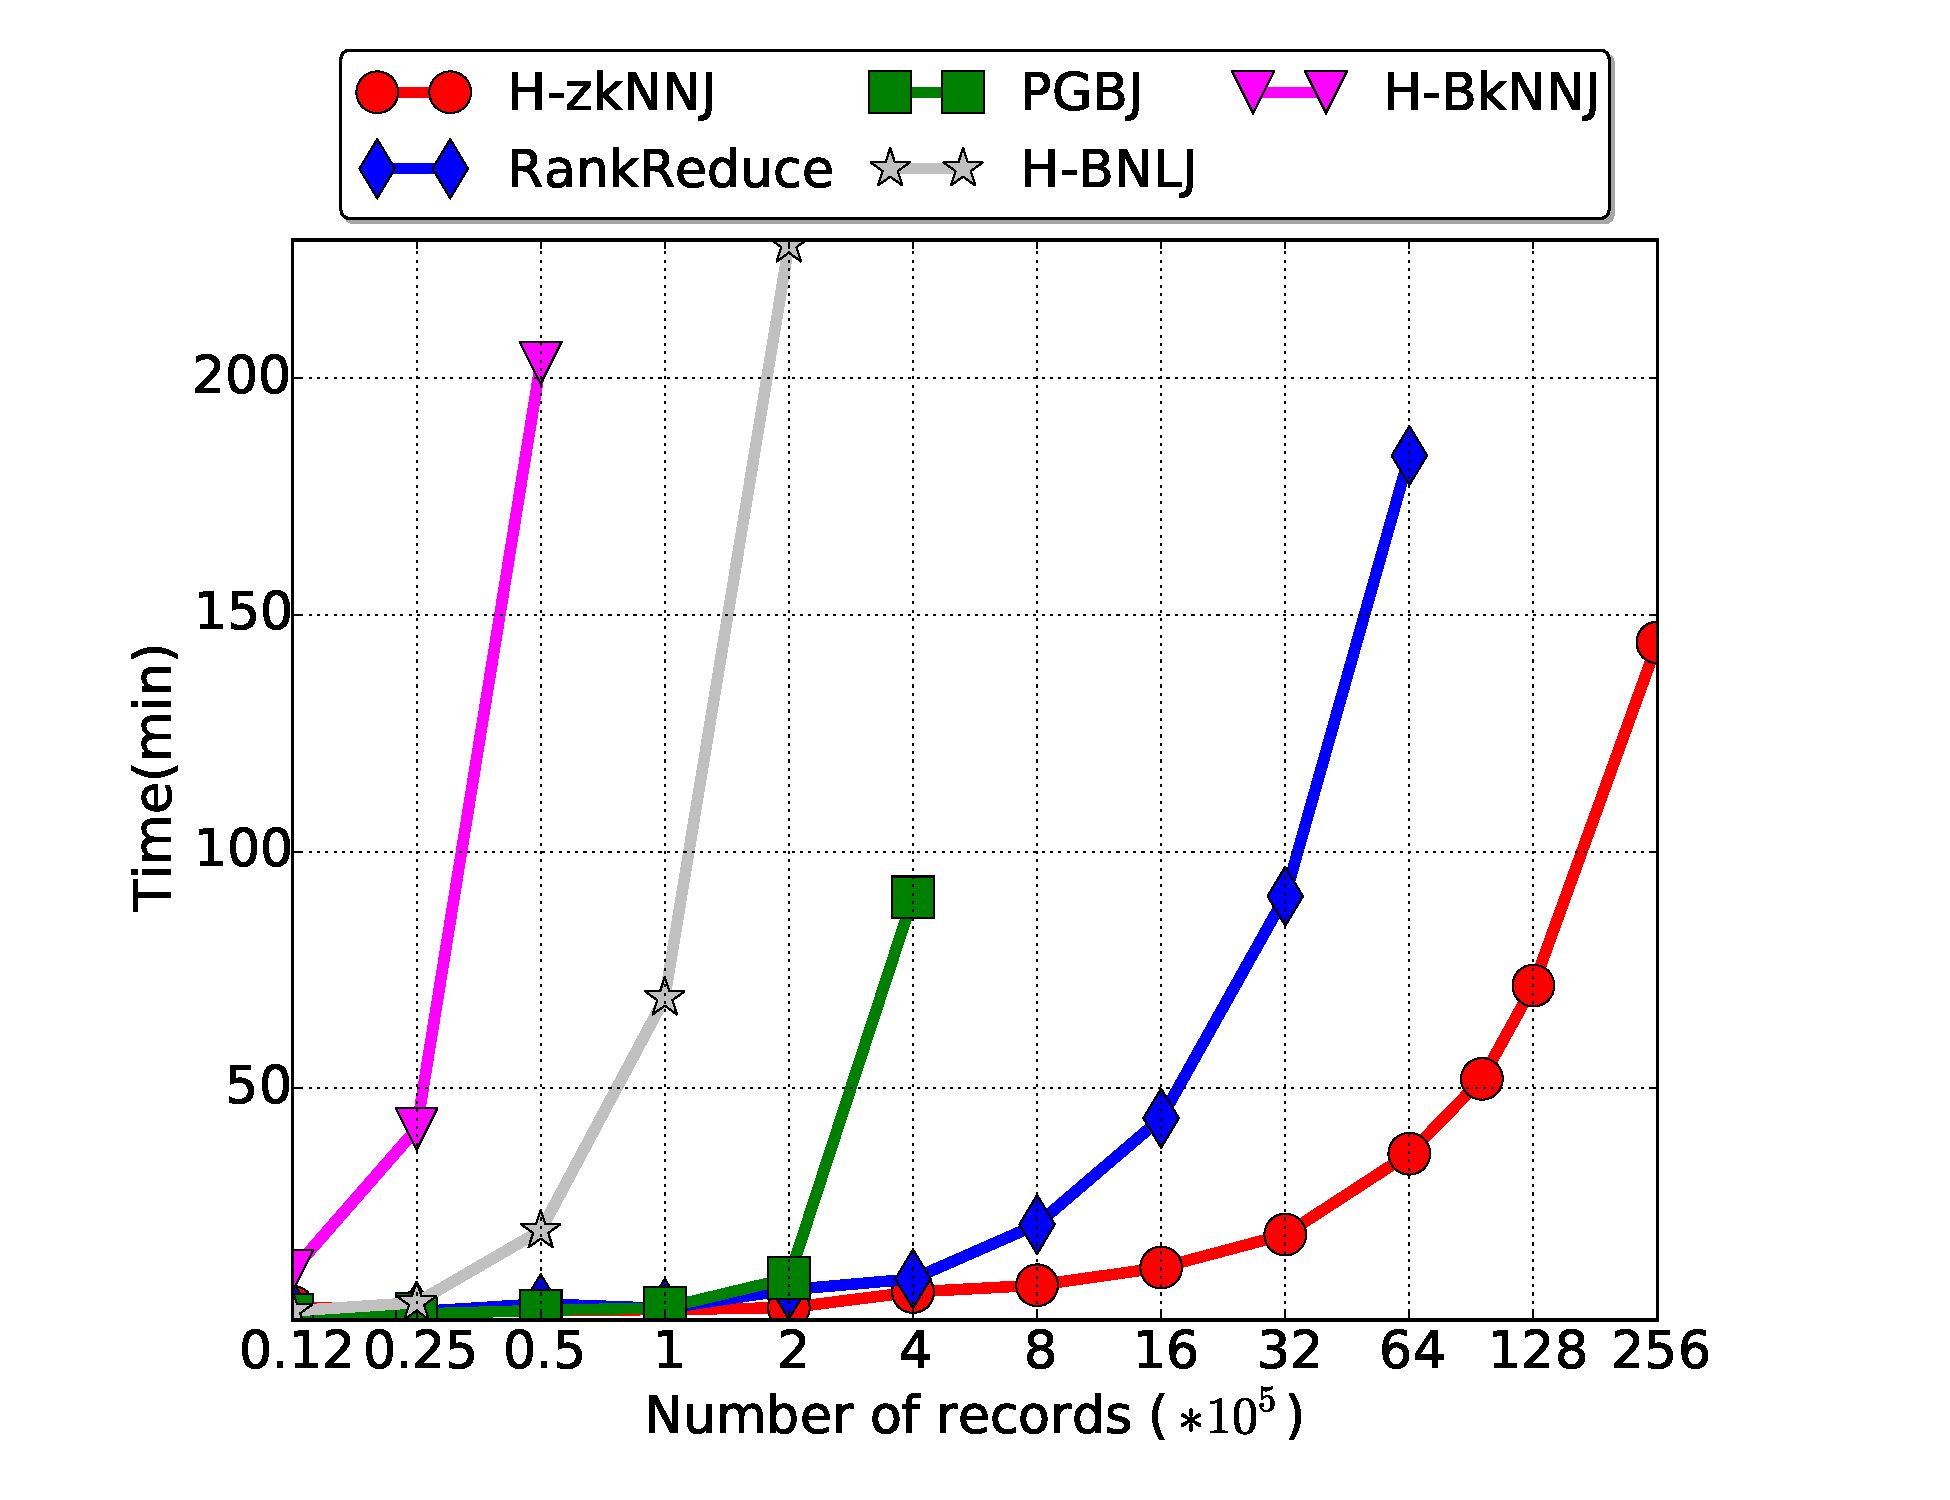
\includegraphics[width=\textwidth]{time.pdf} 
		\caption{Time}
		\label{fig:geo_data_time}
	\end{subfigure}%
	\begin{subfigure}[b]{0.35\textwidth}
		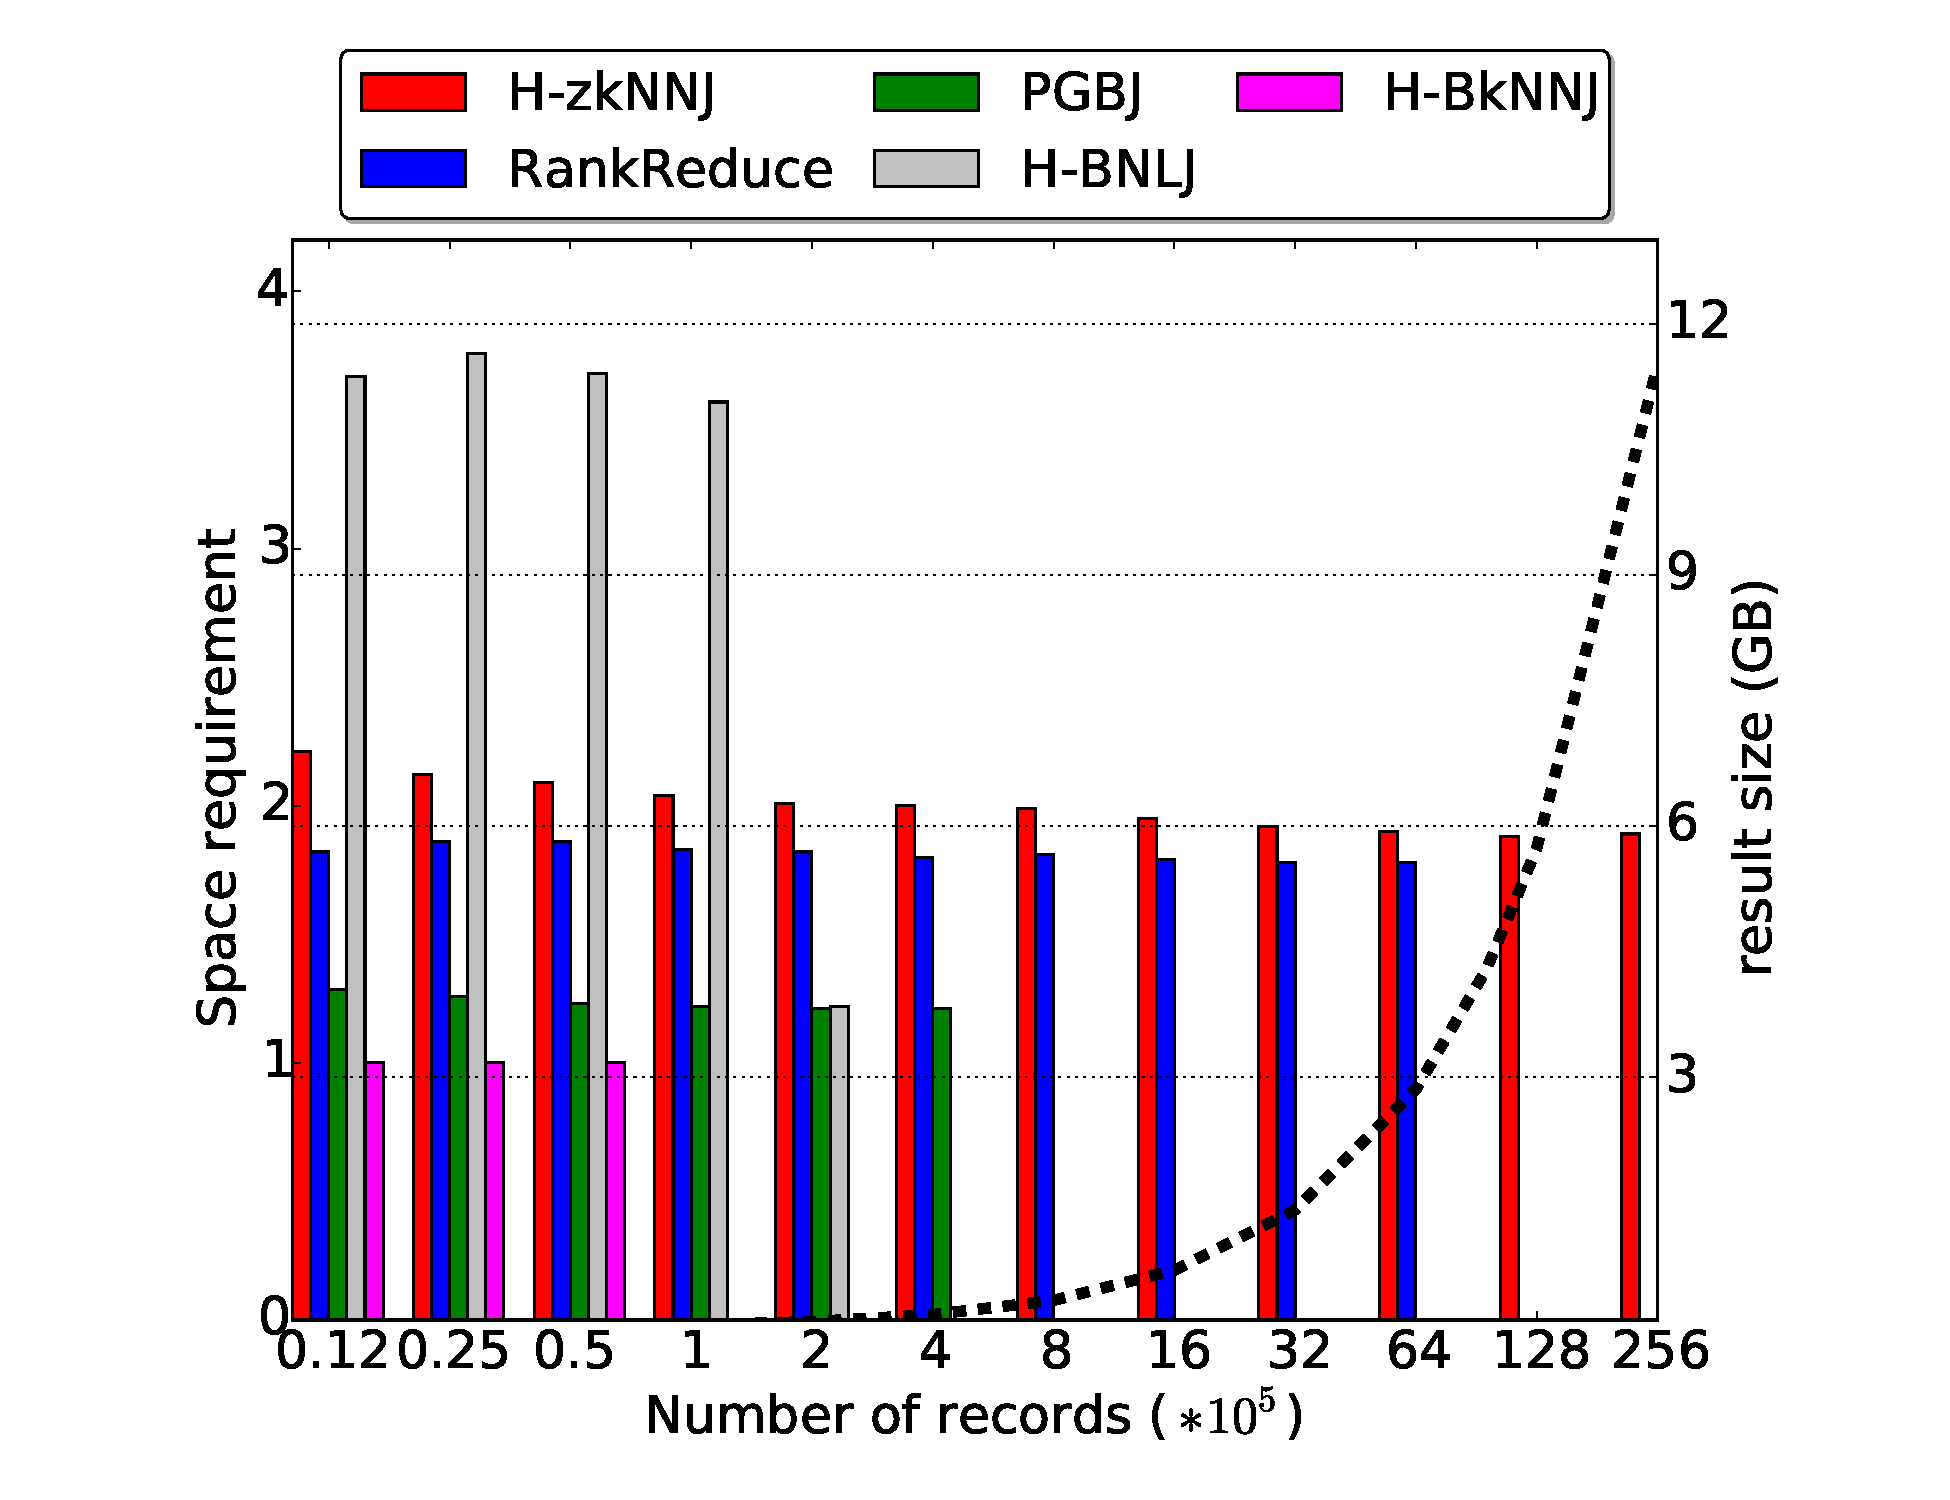
\includegraphics[width=\textwidth]{memory.pdf} 
		\caption{Result size and Disk Usage}
		\label{fig:geo_data_memory}
	\end{subfigure}%
	\begin{subfigure}[b]{0.35\textwidth}
		\includegraphics[width=\textwidth]{accuracy.pdf} 
		\caption{Recall and Precision \label{fig:geo_data_acc}}
	\end{subfigure}%
	\caption{Geo dataset impact of the data set size \label{geo_dataset}}
\end{figure*}


For all experiments in this section, we used the parameters described in Table~\ref{table:parameters_geo}.
Details regarding each parameter can be found in sections \ref{data_preprocessing} and  \ref{partitioning}. For 
RankReduce, the value of $W$ was adapted to get the best performance from each dataset. For datasets up to $16*10^5$
records, $W=32*10^{5}$, up to $25*10^{5}$ records, $W=25*10^{5}$ and finally, $W=15*10^{5}$ for the rest of the 
experiments. 

% shown in Table~\ref{table:parameters_geo}.
\begin{table}[ht]
\begin{center}{\renewcommand{\arraystretch}{1.2} % to prevent equation from being chopped 
\begin{tabular}{|c|c|c|c|}
\hline
\textbf{Algorithm} & \textbf{Partitioning} & \textbf{Reducers} & \textbf{Configuration}  \\ \hline
\HBNLJ             & 10 partitions  & 100 reducers & \\ \hline
\VO               & 3000 pivots     & 25 reducers       & \begin{tabular}[c]{@{}c@{}}k-means \\ + greedy\end{tabular} 
\\ \hline
\LSH          & $W = \left\{
\begin{array}{l}  
	32*10^{5}\\    
    25*10^{5}\\
	15*10^{5}\\
\end{array}\right.$
%$32*10^{5}$
% \TODO{this is plustot the size of bucket but not the number of partition. ??}           
& 25 reducers       & \begin{tabular}[c]{@{}c@{}}L = 2\\ M = 7\end{tabular}       \\ \hline
\Z~           & 10 partitions         & 30 reducers       & 3 shifts, 
p=10                                                     \\ \hline
\end{tabular}
}
\caption{Algorithm parameters \label{table:parameters_geo} for geographic dataset}
\end{center}
\end{table}


\subsubsection{Impact of input data size}
Our first set of experiments measures the impact of the data size on execution time, disk space and recall. 
Figure~\ref{fig:geo_data_time} shows the global computing time of all algorithms, varying 
the number of records from $0.125 * 10^{5}$ to $256 * 10^{5}$. The global computing time increases more or less 
exponentially for all algorithms, but only \Z~and \LSH~can process medium to large datasets. For 
small datasets, \VO~can compute an exact solution as fast as the other algorithms. 


Figure~\ref{fig:geo_data_memory} shows the space requirement of each algorithm as a function of the final output size. 
To 
reduce the footprint of each run, intermediate data are compressed. For example, for 
\HBNLJ, the size of intermediate data is $2.6$ times bigger than the size of output data. Overall, the algorithms with 
the
lowest space requirements are \LSH~and \VO.

Figure~\ref{fig:geo_data_acc} shows the recall and precision of the two approximate algorithms, \Z~and \LSH. Since \Z~
always return $k$ elements, its precision and recall are identical. 
As the number of records increases, its recall decreases, while still being high, because of the 
space filling curves used in the preprocessing phase.
On the other hand, the recall of \LSH~is always lower than its precision because it outputs less than $k$ elements. It
benefits from larger datasets because more data end up in the same bucket, increasing the 
number of candidates. Overall, the quality of \LSH~was found to be better than \Z~on the Geo dataset. 

%\input{parts/exp-dim-figure.tex}
\subsubsection{Impact of k}
Changing the value of $k$ can have a significant impact on the performance of some of the kNN 
algorithms. We experimented on a dataset of $2*10^5$ records (only $5*10^4$ for \HBNLJ~ 
for performance reasons) with values for $k$ varying from 2 to 512. Results are shown in 
Figure~\ref{fig:geo_impact_k} using a logarithmic scale on the x-axis.

First, we observe a global increase in computing time (Figure~\ref{fig:geo_k_time}) which matches the complexity 
analysis performed earlier. 
As $k$ increases, the performance of \Z, compared to the other advanced algorithms, decreases. This is due to the 
necessary replication of the $z$-values of $S$ throughout the partitions to find enough candidates: the core 
computation is thus much more complex. 

%%% generated by A4-ratioByK.py
\begin{figure*}[htp]
	\centering
	\begin{subfigure}[b]{0.35\textwidth}
		\includegraphics[width=\textwidth]{k_time.pdf} 
		\caption{Time\label{fig:geo_k_time}}       
	\end{subfigure}%
	\begin{subfigure}[b]{0.35\textwidth}
		\includegraphics[width=\textwidth]{k_memory.pdf} 
		\caption{Result size and Disk Usage\label{fig:geo_k_memory} }
	\end{subfigure}%
	\begin{subfigure}[b]{0.35\textwidth}
		\includegraphics[width=\textwidth]{k_accuracy.pdf} 
		\caption{Recall and Precision \label{fig:geo_k_acc}}            
	\end{subfigure}%
	\caption{ Geo dataset with 200k records (50k for H-BNLJ), impact of $K$  }
	\label{fig:geo_impact_k}
\end{figure*}

Second, the algorithms can also be distinguished considering their disk usage, visible on 
Figure ~\ref{fig:geo_k_memory}. The global tendency is that the ratio of intermediate data size over the final data 
size decreases. This means that for each algorithm the final 
data size grows faster than the intermediate data size. As a consequence, there is no particular algorithm that 
suffers from such a bottleneck at this point.
\VO~is \ the most efficient from this aspect. Its replication of data occurs independently of the number of 
selected neighbors. Thus, increasing $k$ has a small impact on this algorithm, both in computing time and space 
requirements. On this figure, an interesting observation can also be made for \Z. For $k=2$, it has by far the 
largest disk
usage but becomes similar to the others for larger values. 
This is because \Z~creates a lot of intermediate data (copies of the initial dataset, vectors for the space 
filling curve, sampling...) irrespective of the value of $k$. As $k$ increases, so does the output size, mitigating the 
impact of these intermediate data. 

Surprisingly, changing $k$ has a different impact on the recall of the approximate kNN methods, as can be seen on 
Figure~\ref{fig:geo_k_acc}.
For \LSH, increasing $k$ has a negative impact on the recall which sharply decreases when $k\geq 64$. This is
because the window parameter ($W$) of LSH was set at the beginning of the experiments to achieve the best performance for this
particular dataset. However, it was not modified for various of $k$. Thus it became less optimal as $k$ increased. This 
shows there is a link between global parameters such 
as $k$ and parameters of the LSH process. When using \Z, 
increasing $k$  improves the precision: the probability to have incorrect points is reduced as there are more 
candidates in a single partition. 

\subsubsection{Communication Overhead}
Our last set of experiments looks at inter-node communication by measuring the amount of data transmitted during the
shuffle phase (Figure~\ref{fig:geo_communication}). The goal is to compare these measurements with the theoretical 
analysis in Section~\ref{section:global_complexity}, 

%%%% Generated with   2-time.py  and A4-ratioByK.py
\begin{figure*}[htp]
	\centering
	\begin{subfigure}[b]{0.48\textwidth}
		\includegraphics[width=\textwidth]{shuffle.pdf} 
		\caption{Impact of the data set size\label{fig:geo_data_shuffle}}
	\end{subfigure}%
	\begin{subfigure}[b]{0.48\textwidth}
		\includegraphics[width=\textwidth]{k_shuffle.pdf} 
		\caption{Impact of $K$ with $2*10^5$ records ($0.5*10^5$ for H-BNLJ) \label{fig:geo_k_shuffle}}
	\end{subfigure}%
	\caption{Geo dataset, communication overhead \label{fig:geo_communication}}      
\end{figure*}

\emph{Impact of data size.} For Geo dataset (Figure~\ref{fig:geo_data_shuffle}), \HBNLJ~has indeed a lot of 
communication. For a dataset of $1*10^5$ records, the shuffle phase transmits almost $4$ times the original size.
Both \LSH~and \Z~have a constant factor of $1$ because of the duplication of the original 
dataset
to improve the recall. The most efficient algorithm is \VO~for two reasons. First it does not duplicate the 
original dataset and second, it relies on various grouping strategies to minimize replication.

\emph{Impact of k.}
We have performed another set of experiments, with a fixed dataset of $2*10^5$ records (only $0.5*10^5$ for \HBNLJ). 
The results can be seen in Figure~\ref{fig:geo_k_shuffle}. For different values of $k$, we have a similar hierarchy 
than with the data size. For \LSH~and \Z, the shuffle increases linearly because the number of candidates in the second 
phase depends on $k$. Moreover \Z~also replicates $k$ previous and succeeding elements in the first phase, and because 
of that, its overhead becomes significant for large $k$. Finally in \VO, $k$ has no impact on the shuffle phase.

%\subsection{Image Feature Descriptors (SURF) dataset}
\label{section:surf_dataset}
We now investigate whether the dimension of input data has an impact on the kNN algorithms using the SURF dataset.
We used the Euclidian distance between descriptors to measure image similarity. 
For all experiments in this section, the parameters mentioned in Table~\ref{table:parameters} are used.
\begin{table}[h]
\begin{center}{\renewcommand{\arraystretch}{1.2}
\begin{tabular}{|c|c|c|c|}
\hline
\textbf{Algorithm} & \textbf{Partitioning} & \textbf{Reducers} & 
\textbf{Configuration}                                              \\ \hline
\HBNLJ            & 10 partitions         & 100 reducers      
&                                                             \\ \hline
\VO               & 3000 pivots           & 25 reducers       & \begin{tabular}[c]{@{}c@{}}k-means \\ + 
geo\end{tabular} \\ \hline
\LSH         & W = $10^7$     & 25 reducers       & \begin{tabular}[c]{@{}c@{}}L 
= 5\\ M = 7\end{tabular}       \\ \hline
\Z~           & 6 partitions         & 30 reducers       & 5 shifts                                                    
\\ \hline
\end{tabular}
}
\caption{Algorithm parameters \label{table:parameters} for SURF dataset}
\end{center}
\end{table}

%\input{parts/exp-surf-figure.tex}


%%%% Generated by B00-surf.py
\begin{figure*}[htp]
	\centering
	\begin{subfigure}[b]{0.35\textwidth}
		% \fbox{
		\includegraphics[width=\textwidth]{img-perf/surf/data/time.pdf}
		% }
		\caption{Time\label{fig:surf_data_time}}    
	\end{subfigure}%
	\begin{subfigure}[b]{0.35\textwidth}
		%\fbox{
		\includegraphics[width=\textwidth]{img-perf/surf/data/memory.pdf}
		%}
		\caption{Result size and Disk Usage\label{fig:surf_data_memory}}
	\end{subfigure}%       
	\begin{subfigure}[b]{0.35\textwidth}
		%\fbox{
		\includegraphics[width=\textwidth]{img-perf/surf/data/accuracy.pdf}
		%}
		\caption{Recall and Precision\label{fig:surf_data_acc}}        
	\end{subfigure}%  
	\caption{Surf, impact of the dataset size
		%\\ \small {Parameters : \textbf{HBNLJ} : 10partitions, \textbf{PGBJ}:$3*10^{3} pivots$, Geo grouping, kmeans 
		%sample, \textbf{RankReduce}: $L=5,M=7,W=10^{7}$ HZKNNJ : $3shift$} 
		\label{fig:surf_dataset} }
\end{figure*}

%%%% Generated by A4-ratioByK-SURF.py
\begin{figure*}[htp]
	\centering
	\begin{subfigure}[b]{0.35\textwidth}
		%\fbox{
		\includegraphics[width=\textwidth]{img-perf/surf/k/time.pdf} 
		%}
		\caption{Time\label{fig:surf_k_time} }
		
	\end{subfigure}%
	\begin{subfigure}[b]{0.35\textwidth}
		% \fbox{
		\includegraphics[width=\textwidth]{img-perf/surf/k/memory.pdf} 
		%}
		\caption{Result size and Disk Usage\label{fig:surf_k_memory}}
	\end{subfigure}%
	\begin{subfigure}[b]{0.35\textwidth}
		%\fbox{
		\includegraphics[width=\textwidth]{img-perf/surf/k/accuracy.pdf}
		%}
		\caption{Recall and Precision\label{fig:surf_k_acc}}
		
	\end{subfigure}%
	\caption{Surf dataset with 50k records, impact of $K$,
		%\\ \small{Parameters : \textbf{HBNLJ} : 10partition, \textbf{PGBJ}:$3*10^3 pivots$, Geo grouping, kmeans 
		%sample,\textbf{RankReduce}: $L=5,M=7,W=10^7$ HZKNNJ : $3shift$}  
		\label{fig:surf_impact_k}}
\end{figure*}


\subsubsection{Impact of input data size}

Results of experiments when varying the number of descriptors are shown in Figure~\ref{fig:surf_dataset} using a log 
scale on the x-axis. We omitted \HBK~as it could not process the data in reasonable time.
In Figure~\ref{fig:surf_data_time}, we can see that the execution time of the algorithms follows globally 
the same trend as 
with the Geo dataset, except for \VO. It is a computational intensive algorithm because the replication process implies 
calculating a lot of Euclidian distances. When in dimension 128, this part tends to dominate the overall computation 
time. Regarding disk usage (Figure~\ref{fig:surf_data_memory}), \Z~is very high because  we had to increase the number 
of shifted copies from $3$ to $5$ to 
improve the recall. Indeed, compared to the Geo dataset, it is very low (Figure~\ref{fig:surf_data_acc}). Moreover, as 
the number of descriptors 
increases, \Z~goes from 30\% to 15\% recall. As explained before, the precision was found to be equal to the recall, which means the 
algorithm always returned $k$ results. This, together with the improvement using more shifts, proves that the 
space filling curves using in \Z~are less efficient with high dimension data. 
%A solution is to 
%increase the number of shifted copies from $3$ to $5$. But the impact of time is double and no very efficient, it 
%increases just to $0.05$ the recall . \TODO{I'm confused, was the shift increased or not?}

\subsubsection{Impact of $k$}

Figure \ref{fig:surf_impact_k} shows the impact of different values of $k$ on the algorithms using a logarithmic scale 
on the x-axis.
Again, since for \HBNLJ~and \Z, the complexity of the sorting phase is dependent on $k$, we can observe a 
corresponding increase of the execution time (Figure~\ref{fig:surf_k_time}). For 
\LSH, the time varies a lot depending on $k$. This is because of the stochastic nature of the projection used in 
LSH. It can lead to buckets containing different number of elements, creating a load imbalance and some values
of $k$ naturally lead to a better load balancing. \VO~is very dependent on the value of $k$ because of the grouping 
phase. Neighboring cells are added until there are enough elements to eventually identify the $k$ nearest neighbors. 
As a consequence, a large $k$ will lead to larger group of cells and increase the computing time. 

Figure~\ref{fig:surf_k_memory} shows the effect of $k$ on disk usage. \Z~starts with a very high ratio of 74 
(not showed on the Figure) and 
quickly reduces to more acceptable values. 
 \LSH~also experiences a similar pattern to a lesser extend. As opposed to the Geo dataset, SURF 
descriptors cannot be efficiently compressed, leading to large intermediate files.

Finally, Figure~\ref{fig:surf_k_acc} shows the effect of $k$ on the recall. As $k$ increases, the recall and precision 
of \LSH~ decreases for the same reason as with the Geo dataset. Also, for large $k$, the recall becomes lower
than the precision because we get less than $k$ results. The precision of \Z~decreases but eventually shows an upward 
trend. The increased number of requested neighbors increases the number of preceding and
succeeding points copied, slightly improving the recall.
%  the number of searched $k$ reduce the probability to make 
%mistake and, 
%contrarily to \LSH, no $k$ is missing in the result (recall = precision) \TODO{Rewrite}

\subsubsection{Communication Overhead}
With the SURF dataset, we get a very different behavior than with the Geo dataset. The shuffle phase of \VO~is very 
costly (Figure~\ref{fig:surf_data_shuffle}). This is an indication of large replications incurred by the large 
dimension of the data and a poor choice of pivots. When they are too close to each other, entire cells have to be 
replicated during the grouping phase.

%%%% Generated by B00-surf.py and A4-ratioByK-SURF.py
\begin{figure*}[htp]
	\centering
	\begin{subfigure}[b]{0.48\textwidth}
		\includegraphics[width=\textwidth]{img-perf/surf/data/shuffle.pdf}
		\caption{Surf, impact of the dataset size\label{fig:surf_data_shuffle}}        
	\end{subfigure}% 
	\begin{subfigure}[b]{0.48\textwidth}
		\includegraphics[width=\textwidth]{img-perf/surf/k/shuffle.pdf} 
		\caption{Surf dataset with 50k records, impact of $K$,\label{fig:surf_k_shuffle}}
	\end{subfigure}%
	\caption{Communication overhead for the Surf dataset}      
\end{figure*}


For \LSH~the shuffle is decreased but stay important, essentially because of the replication factor of $5$. Finally,
the shifts of original data in \Z~lead to a large communication overhead. 


Considering now $k$, we have the same behavior we observed with the Geo dataset. The only difference is \VO~which now exhibits a
large communication overhead (Figure~\ref{fig:surf_k_shuffle}). This is again because of the choice of pivots and 
the grouping of the cells. However, this overhead remains constant, irrespective of $k$. 
\subsection{Image Feature Descriptors (SURF) dataset}
\label{section:surf_dataset}
We now investigate whether the dimension of input data has an impact on the kNN algorithms using the SURF dataset.
We used the Euclidian distance between descriptors to measure image similarity. 
For all experiments in this section, the parameters mentioned in Table~\ref{table:parameters} are used.
\begin{table}[h]
\begin{center}{\renewcommand{\arraystretch}{1.2}
\begin{tabular}{|c|c|c|c|}
\hline
\textbf{Algorithm} & \textbf{Partitioning} & \textbf{Reducers} & 
\textbf{Configuration}                                              \\ \hline
\HBNLJ            & 10 partitions         & 100 reducers      
&                                                             \\ \hline
\VO               & 3000 pivots           & 25 reducers       & \begin{tabular}[c]{@{}c@{}}k-means \\ + 
geo\end{tabular} \\ \hline
\LSH         & W = $10^7$     & 25 reducers       & \begin{tabular}[c]{@{}c@{}}L 
= 5\\ M = 7\end{tabular}       \\ \hline
\Z~           & 6 partitions         & 30 reducers       & 5 shifts                                                    
\\ \hline
\end{tabular}
}
\caption{Algorithm parameters \label{table:parameters} for SURF dataset}
\end{center}
\end{table}

%\input{parts/exp-surf-figure.tex}


%%%% Generated by B00-surf.py
\begin{figure*}[htp]
	\centering
	\begin{subfigure}[b]{0.35\textwidth}
		% \fbox{
		\includegraphics[width=\textwidth]{time_surf.pdf}
		% }
		\caption{Time\label{fig:surf_data_time}}    
	\end{subfigure}%
	\begin{subfigure}[b]{0.35\textwidth}
		%\fbox{
		\includegraphics[width=\textwidth]{memory_surf.pdf}
		%}
		\caption{Result size and Disk Usage\label{fig:surf_data_memory}}
	\end{subfigure}%       
	\begin{subfigure}[b]{0.35\textwidth}
		%\fbox{
		\includegraphics[width=\textwidth]{accuracy_surf.pdf}
		%}
		\caption{Recall and Precision\label{fig:surf_data_acc}}        
	\end{subfigure}%  
	\caption{Surf, impact of the dataset size
		%\\ \small {Parameters : \textbf{HBNLJ} : 10partitions, \textbf{PGBJ}:$3*10^{3} pivots$, Geo grouping, kmeans 
		%sample, \textbf{RankReduce}: $L=5,M=7,W=10^{7}$ HZKNNJ : $3shift$} 
		\label{fig:surf_dataset} }
\end{figure*}

%%%% Generated by A4-ratioByK-SURF.py
\begin{figure*}[htp]
	\centering
	\begin{subfigure}[b]{0.35\textwidth}
		%\fbox{
		\includegraphics[width=\textwidth]{time_k.pdf} 
		%}
		\caption{Time\label{fig:surf_k_time} }
		
	\end{subfigure}%
	\begin{subfigure}[b]{0.35\textwidth}
		% \fbox{
		\includegraphics[width=\textwidth]{memory_k.pdf} 
		%}
		\caption{Result size and Disk Usage\label{fig:surf_k_memory}}
	\end{subfigure}%
	\begin{subfigure}[b]{0.35\textwidth}
		%\fbox{
		\includegraphics[width=\textwidth]{accuracy_k.pdf}
		%}
		\caption{Recall and Precision\label{fig:surf_k_acc}}
		
	\end{subfigure}%
	\caption{Surf dataset with 50k records, impact of $K$,
		%\\ \small{Parameters : \textbf{HBNLJ} : 10partition, \textbf{PGBJ}:$3*10^3 pivots$, Geo grouping, kmeans 
		%sample,\textbf{RankReduce}: $L=5,M=7,W=10^7$ HZKNNJ : $3shift$}  
		\label{fig:surf_impact_k}}
\end{figure*}


\subsubsection{Impact of input data size}

Results of experiments when varying the number of descriptors are shown in Figure~\ref{fig:surf_dataset} using a log 
scale on the x-axis. We omitted \HBK~as it could not process the data in reasonable time.
In Figure~\ref{fig:surf_data_time}, we can see that the execution time of the algorithms follows globally 
the same trend as 
with the Geo dataset, except for \VO. It is a computational intensive algorithm because the replication process implies 
calculating a lot of Euclidian distances. When in dimension 128, this part tends to dominate the overall computation 
time. Regarding disk usage (Figure~\ref{fig:surf_data_memory}), \Z~is very high because  we had to increase the number 
of shifted copies from $3$ to $5$ to 
improve the recall. Indeed, compared to the Geo dataset, it is very low (Figure~\ref{fig:surf_data_acc}). Moreover, as 
the number of descriptors 
increases, \Z~goes from 30\% to 15\% recall. As explained before, the precision was found to be equal to the recall, which means the 
algorithm always returned $k$ results. This, together with the improvement using more shifts, proves that the 
space filling curves using in \Z~are less efficient with high dimension data. 
%A solution is to 
%increase the number of shifted copies from $3$ to $5$. But the impact of time is double and no very efficient, it 
%increases just to $0.05$ the recall . \TODO{I'm confused, was the shift increased or not?}

\subsubsection{Impact of $k$}

Figure \ref{fig:surf_impact_k} shows the impact of different values of $k$ on the algorithms using a logarithmic scale 
on the x-axis.
Again, since for \HBNLJ~and \Z, the complexity of the sorting phase is dependent on $k$, we can observe a 
corresponding increase of the execution time (Figure~\ref{fig:surf_k_time}). For 
\LSH, the time varies a lot depending on $k$. This is because of the stochastic nature of the projection used in 
LSH. It can lead to buckets containing different number of elements, creating a load imbalance and some values
of $k$ naturally lead to a better load balancing. \VO~is very dependent on the value of $k$ because of the grouping 
phase. Neighboring cells are added until there are enough elements to eventually identify the $k$ nearest neighbors. 
As a consequence, a large $k$ will lead to larger group of cells and increase the computing time. 

Figure~\ref{fig:surf_k_memory} shows the effect of $k$ on disk usage. \Z~starts with a very high ratio of 74 
(not showed on the Figure) and 
quickly reduces to more acceptable values. 
 \LSH~also experiences a similar pattern to a lesser extend. As opposed to the Geo dataset, SURF 
descriptors cannot be efficiently compressed, leading to large intermediate files.

Finally, Figure~\ref{fig:surf_k_acc} shows the effect of $k$ on the recall. As $k$ increases, the recall and precision 
of \LSH~ decreases for the same reason as with the Geo dataset. Also, for large $k$, the recall becomes lower
than the precision because we get less than $k$ results. The precision of \Z~decreases but eventually shows an upward 
trend. The increased number of requested neighbors increases the number of preceding and
succeeding points copied, slightly improving the recall.
%  the number of searched $k$ reduce the probability to make 
%mistake and, 
%contrarily to \LSH, no $k$ is missing in the result (recall = precision) \TODO{Rewrite}

\subsubsection{Communication Overhead}
With the SURF dataset, we get a very different behavior than with the Geo dataset. The shuffle phase of \VO~is very 
costly (Figure~\ref{fig:surf_data_shuffle}). This is an indication of large replications incurred by the large 
dimension of the data and a poor choice of pivots. When they are too close to each other, entire cells have to be 
replicated during the grouping phase.

%%%% Generated by B00-surf.py and A4-ratioByK-SURF.py
\begin{figure*}[htp]
	\centering
	\begin{subfigure}[b]{0.48\textwidth}
		\includegraphics[width=\textwidth]{shuffle_surf.pdf}
		\caption{Surf, impact of the dataset size\label{fig:surf_data_shuffle}}        
	\end{subfigure}% 
	\begin{subfigure}[b]{0.48\textwidth}
		\includegraphics[width=\textwidth]{shuffle_k.pdf} 
		\caption{Surf dataset with 50k records, impact of $K$,\label{fig:surf_k_shuffle}}
	\end{subfigure}%
	\caption{Communication overhead for the Surf dataset}      
\end{figure*}


For \LSH~the shuffle is decreased but stay important, essentially because of the replication factor of $5$. Finally,
the shifts of original data in \Z~lead to a large communication overhead. 


Considering now $k$, we have the same behavior we observed with the Geo dataset. The only difference is \VO~which now exhibits a
large communication overhead (Figure~\ref{fig:surf_k_shuffle}). This is again because of the choice of pivots and 
the grouping of the cells. However, this overhead remains constant, irrespective of $k$. 


\subsection{Impact of Dimension and Dataset}
We now analyze the behavior of these algorithms according to the dimension of  data. Since 
some algorithms are dataset dependent (i.e the spatial distribution of data has an impact on 
the outcome), we need to separate data distribution from the dimension. Hence, we use two
different kinds of datasets for these experiments. First, we use real world data of various 
dimensions\footnote{archive.ics.uci.edu/ml/datasets.html}. Second, we have built specific datasets by generating 
uniformly distributed data to limit the impact of clustering. All the experiments were performed using 
$0.5*10^5$ records and $k=20$. 
 
 



%%%% Generated by 3-dim.py
\begin{figure*}[ht]
	\centering
	\begin{subfigure}[b]{0.5\textwidth}
		\includegraphics[width=1\textwidth]{datasettime.pdf} 
		\caption{Execution time% for real datasets of various dimensions%
		}
		\label{fig:dim_time}
	\end{subfigure}\begin{subfigure}[b]{0.5\textwidth}
	\includegraphics[width=1\textwidth]{datasetacc.pdf} 
	\caption{Recall and Precision %for real datasets of various dimensions%
	}
	\label{fig:dim_acc}
\end{subfigure}%
\caption{Real datasets of various dimensions}
\label{fig:dim_real}
\end{figure*} 

\begin{figure*}[ht]
	\centering
	\begin{subfigure}[b]{0.5\textwidth}
		\includegraphics[width=1\textwidth]{randtime.pdf} 
		\caption{Execution time% for real datasets of various dimensions%
		}
		\label{fig:rand_time}
	\end{subfigure}\begin{subfigure}[b]{0.5\textwidth}
	
	\includegraphics[width=1\textwidth]{randacc.pdf} 
	\caption{Recall and Precision}
	\label{fig:rand_acc}
\end{subfigure}%
\caption{Generated datasets of various dimensions}
\label{fig:dim_rand}
\end{figure*} 


Since \HBNLJ~relies on the dot product, it is not dataset dependent and its execution time increases
with the dimension as seen on Figures \ref{fig:dim_time} and \ref{fig:rand_time}. 

\VO~is heavily dependent on data distribution and on the choice of pivots to build clusters of 
equivalent size which improves parallelism. The comparison of execution times for the datasets 
\emph{128-sift} and \emph{281-blog} in Figure \ref{fig:dim_time} shows that, although the dimension
of data increases, the execution time is greatly reduced. Nonetheless, the clustering phase of the algorithm performs a 
lot of dot product operations which makes it dependent on the dimension, as can be seen in Figure \ref{fig:rand_time}. 

\Z~is an algorithm that depends on spatial dimension. Very efficient for low dimension, its 
execution time increases with the dimension (Figure \ref{fig:rand_time}). A closer 
analysis shows that all phases see their execution time increase. However, the overall time is 
dominated by the first phase (generation of shifted copies and partitioning) whose time complexity
sharply increases with dimension. Data distribution has 
an impact on the recall which gets much lower than the precision for some datasets (Figure~\ref{fig:dim_acc}).
With generated dataset (Figure~\ref{fig:rand_acc}), both recall and precision are identical and initially very high. 
However as dimension increases, the recall decreases because of the projection. 

Finally, \LSH~is both dependent on the dimension and distribution of data. Experiments with the real datasets have 
proved to be difficult because of the various parameters of the algorithm to obtain the requested number of 
neighbors without dramatically increasing the execution time (see discussion in Section~\ref{rankreduceanalysis}). 
Despite our efforts, the precision was very low for some datasets, in particular \emph{28-higgs}. 
Using the generated datasets, we see that its execution time increases with the dimension (Figure~\ref{fig:rand_time}) 
but its recall remains stable (Figure~\ref{fig:rand_acc}). 

\subsection{Practical Analysis}
In this section, we analyze the algorithms from a practical point of view, outlying their sensitivity to 
the dataset, the environment or some internal parameters.   
\subsubsection{H-BkNNJ}
%HBKNNJ
The main drawback of \HBK~is that only the Map phase is in parallel. In addition, the optimal parallelization 
is subtle to achieve because the optimal number of nodes to use is defined by  
$\frac{input\,size}{input\,split\,size}$. This algorithm is clearly not suitable for large datasets but because of its 
simplicity, it can, nonetheless, be used when the amount of data is small.  

\subsubsection{H-BNLJ}
In \HBNLJ, both the Map and Reduce phases are in parallel, but the optimal number of tasks is difficult to 
find. Given a number of partitions $n$, there will be $n^2$ tasks. Intuitively, one would choose a number of 
tasks that is a multiple of the number of processing 
units. The issue with this strategy is that the distribution of the partitions might be unbalanced.
Figure~\ref{fig:lb_hbnlj}
shows an experiment with $6$ partitions and $6^2=36$ tasks, each executed on a reducer. Some reducers will have more elements to process than others, 
slowing the computation.
\begin{figure}[!h]
\centering
   \includegraphics[width=0.4\textwidth]{hbnlj.pdf}
   \caption{H-BNLJ, candidates job, $10^{5}$ records \label{fig:lb_hbnlj}, 6 partitions, Geo dataset}
\end{figure}%

Overall, the challenge with this algorithm is to find the optimal number of partitions for a given dataset. 

\subsubsection{PGBJ} 
A difficulty in \VO~comes from its sampling-based preprocessing techniques because it 
impacts the partitioning and thus the load balancing. This raises many challenges. First, how to choose
the pivots from the initial dataset. The three techniques proposed by the authors, farthest, k-means and 
random, lead to different pivots and different partitions and possibly different executions. We found that 
with  our datasets, both k-means and random techniques
gave the best performance. Second, the number of pivots is also important because
it will impact the number of partitions. A too small or too large number of pivots 
will decrease performance. Finally, another important parameter is the grouping strategy used 
(Section~\ref{pgbj_grouping}).
\begin{figure}[!h]
   \includegraphics[width=0.5\textwidth]{strategy.pdf} 
   \caption{PGBJ, overall time (lines) and Grouping time (bars)\label{fig:pgbj_strategy} with Geo dataset, 3000 pivots, 
   KMeans Sampling}         
\end{figure}
In Figure~\ref{fig:pgbj_strategy}, we can see that the greedy grouping technique has a higher grouping time 
(bars) than the geo grouping technique. 
However, the global computing time (line) using this technique is shorter thanks to the good load balancing. This
is illustrated by Figure~\ref{fig:pgbj_balancing} which shows the distribution of elements processed
by reducers when using geo grouping (\ref{fig:geo_20r}) or greedy grouping (\ref{fig:greedy_20r}).
                  
\begin{figure}[h]
\centering
		\begin{subfigure}[b]{0.25\textwidth}
                \includegraphics[width=\textwidth]{geo_20r_400.pdf}
                \caption{Geo\label{fig:geo_20r}}
                
        \end{subfigure}%
        \begin{subfigure}[b]{0.25\textwidth}
                \includegraphics[width=\textwidth]{greedy_20r_400.pdf}
                \caption{Greedy\label{fig:greedy_20r}}
                
        \end{subfigure}%
        \caption{PGBJ, load balancing \label{fig:pgbj_balancing} with 20 reducers}
\end{figure}                
 
\subsubsection{H-zkNNJ}\label{z-value}
In \Z, the $z$-value transformation leads to information loss. The recall of this algorithm is influenced
by  the nature, the dimension and the size of the input data.
More specifically, this algorithm becomes biased if the distance between initial data is very scattered, and 
the more input data or the higher the dimension, the more difficult it is to draw the space filling curve. To 
improve the recall, the authors propose to create duplicates in the original dataset by shifting data. 
This greatly increases the amount of data to process and has a significant impact on the execution time.

\begin{table*}[ht]
 	\begin{center}\renewcommand{\arraystretch}{1.2}
 		\begin{tabular}{|c|c|c|c|}
 			\hline
 			\textbf{Algorithm}  & \textbf{Advantage}  &  \textbf{Shortcoming}   & \textbf{Typical Usecase} \\
 			 \hline
 			\textbf{H-BkNNJ} 	& 
 				\begin{tabular}[c]{@{}c@{}}
 					Trivial to implement  
 				\end{tabular} & 
 				\begin{tabular}[c]{@{}c@{}}
 					1. Breaks very quickly \\ 
 					2. Optimal parallelism difficult\\ 
 					to achieve a priori
 				\end{tabular} &
 				\begin{tabular}[c]{@{}c@{}}
 			    	Any tiny and low dimension dataset\\
 			    	($\sim$ 25000 records)
 			    \end{tabular} \\ \hline
 			\textbf{H-BNLJ}     &
 				\begin{tabular}[c]{@{}c@{}}
 				 	Easy to implement
 				\end{tabular} & 
 				\begin{tabular}[c]{@{}c@{}}
 				 	1. Slow\\
 				 	2. Very large communication overhead 
 				\end{tabular} & 
 				\begin{tabular}[c]{@{}c@{}}
 				 	Any small/medium dataset\\
 				 	($\sim$ 100000 records)
 				\end{tabular} \\ \hline
 			\textbf{PGBJ}       & 
	 			\begin{tabular}[c]{@{}c@{}}
 				   	1. Exact solution\\ 
 				   	2. Lowest disk usage\\ 
 			       	3. No impact on communication\\
 			       	overhead with the increase of $k$
	 			\end{tabular}        & 
	 			\begin{tabular}[c]{@{}c@{}}
	 				1. Cannot finish in reasonable time\\ 
	 				for large dataset\\ 
	 				2. Poor performance for high\\
	 				dimension data\\
	 				3. Large communication overhead\\
	 				4. Performance highly depends on\\ 
	 				the quality of a priori chosen pivots
	 			\end{tabular} & 
 				\begin{tabular}[c]{@{}c@{}}
 					1. Medium/large dataset for\\
 					low/medium dimension\\
 					2. Exact results
 				\end{tabular} \\ \hline
 			\textbf{H-zkNNJ}    &
	 			\begin{tabular}[c]{@{}c@{}}
	 			    1. Fast\\ 
	 			    2. Does not require a priori parameter\\ 
	 			    tuning \\ 
	 			    3. More precise for large k \\ 
	 			    4. Always give the right number of $k$	 	
	 	        \end{tabular} & 
	 	        \begin{tabular}[c]{@{}c@{}}
	 	        	1. High disk usage\\ 
	 	        	2. Slow for large dimension \\ 
	 	        	3. Very high space requirement ratio \\ 
	 	        	for small values of $k$
 				\end{tabular} & 
 				\begin{tabular}[c]{@{}c@{}}
 					1. Large dataset of small dimension\\
 					2. High values of $k$\\
 			        3. Approximate results
 				\end{tabular} \\ \hline
 			\textbf{RankReduce} & 
 			\begin{tabular}[c]{@{}c@{}}
 				1. Fast\\ 
 				2. Low footprint on disk usage
 			\end{tabular} & 
 			\begin{tabular}[c]{@{}c@{}}
 				1. Fine parameter tuning required with\\ 
 				experimental set up \\
 				2. Multiple hash functions needed for\\
 				acceptable recall \\
 				3. Different quality metrics to consider\\
 				(recall + precision)
 		   \end{tabular}                                           
 			& \begin{tabular}[c]{@{}c@{}}
 				1. Large dataset of any dimension \\
 				2. Approximate results \\
 				3. Room for parameter tuning
 			\end{tabular} \\ \hline
 		\end{tabular}
 		\caption{Summary table for each algorithm in practice}\label{summary_practice}  
 	\end{center}
 \end{table*}

\subsubsection{RankReduce}\label{rankreduceanalysis}
\LSH, with the addition of a third job, can have the best performance of all, provided that it is started with the 
optimal parameters.
The most important ones are $W$, the size of each bucket, $L$, the number of hash families and $M$, the number 
of hash functions in each family. Since they are dependent on the dataset, experiments are 
needed to precisely tune them. In \cite{Dong:2008:MLP:1458082.1458172_full}, the authors suggests this can be achieved 
with a sample dataset and a theoretical model. 
The first important metric to consider is the number of candidates available in each bucket. Indeed, with some 
poorly chosen parameter values, it is possible to have less than $k$ elements in each bucket, making it impossible to 
have enough elements at the end of the computation (there are less than $k$ neighbors in the result). On the opposite, 
having too many candidates in each bucket will increase too much the execution time. 
To illustrate the complexity of the parameter tuning operation, we have run experiments on the Geo and SURF datasets. 
First, Figure~\ref{fig:lsh_tunning_geo} shows that, for the Geo dataset, increasing $W$ improves the recall and the 
precision at the expense of the execution time, up to an optimal before decreasing. This can be explained by looking
at the number of buckets for a given $W$. As $W$ increases, each bucket contains more elements and thus their number 
decreases. As a consequence, the probability to have the correct $k$ neighbors inside a bucket increases, which 
improves the recall. However, the computational load of each bucket also increases.

 
\begin{figure}[!h]
 \centering
          \includegraphics[width=0.5\textwidth]{params_geo_time.pdf} 
         \caption{LSH tuning, Geo dataset, 40k records,  20 nodes}
                \label{fig:lsh_tunning_geo}
\end{figure}
\begin{figure}[!h]
         \centering
       % \begin{subfigure}[b]{0.25\textwidth}
                 \includegraphics[width=0.5\textwidth]{params_surf.pdf} 
                %\caption{lsh tunning surf}
        %\end{subfigure}
         \caption{LSH tuning, SURF dataset, 40k records, 20 nodes}\label{fig:lsh_tunning_surf}
\end{figure}

A similar pattern can be observed with the SURF dataset (Figure~\ref{fig:lsh_tunning_surf}, left), where 
increasing $W$ improves the recall (from 5\% to 35\%) and the precision (from 22\% to 35\%). Increasing 
the number of families $L$ greatly improves both the precision and recall. However, increasing $M$, the
number of hash functions, decreases the number of collisions, reducing execution time but also the recall and 
precision. Overall, finding the optimal parameters for the LSH part is complex and has to be done for every dataset

After finishing all the experiments, we found that the execution time of all algorithms mostly follows the 
theoretical analysis presented in Section~\ref{sec:analysis}. However, as expected, the computationally intensive
part, which could not be expressed analytically, has proved to be very sensitive to a lot of different factors.
The dataset itself, through its dimension and the data distribution, but also the parameters of some of the 
pre-processing steps. The magnitude of this sensitivity and its impact on metrics such as recall and precision
could not have been inferred without thorough experiments. 


\subsection{Lessons Learned}

The first aspect is related to load balance. \HBNLJ~actually cannot guarantee load balancing, because of the random 
method it uses to split data. For \VO, Greedy grouping gives a better load balance than Geo grouping, at 
the cost of an increased duration of the grouping phase. At 
the same time, our experiments also confirm that \Z~and \LSH, which use size based 
partitioning strategies, have a very good load balance, with a very small deviation of the completion time of each 
task. %\TODO{3s out of how long? we need to put a \% ---done}

Regarding disk usage, generally speaking, \VO~has the lowest disk space requirement, while \Z~has the largest for small
$k$ values. However, for large $k$, the space requirement of all algorithms becomes similar. 
%\TODO{better word, comparable en francais}.

The communication overhead of \VO~is very sensitive to the choice of pivots. 

The data are another important aspect affecting the performance of the algorithms. As expected, all the 
algorithms' performance decreases as the dimension of data increases. However, what exceeded the prediction of the 
theoretical analysis is that the dimension is really a curse for \VO~. Because of the cost of computing distances in 
the pre-processing phase, its performance becomes really poor, sometimes worse than \HBNLJ. \Z~also suffers from the 
dimension, which decreases its recall. However, the major impact comes from the distribution of data. 

In addition, the overall performance is also sensitive to some specific parameters, especially for \LSH. Its 
performance depends a lot on some parameter tuning, which requires extensive experiments.

Based on the experimental results, we summarize the advantages, disadvantages and suitable usage scenarios for each 
algorithm, in Table~\ref{summary_practice}.

%\section{Conclusion}
In this paper, we have studied the existing systems to perform the kNN operation in the context of MapReduce. 
We have first approached this problem from a workflow 
point of view. We have pointed out that all solutions follow three main steps to compute kNN over MapReduce, namely the pre-processing of data,
the partitioning and the actual computation. We have listed and explained the different algorithms which could be chosen 
for each step, and developed their pros and cons.
In a second stage, we have further analyzed existing systems by reviewing their main properties, in terms of load balancing, accuracy of the computation, 
and overall complexity. Above all, this paper can be seen as a guideline to help selecting 
the most appropriate method to perform the kNN join operation on MapReduce for a particular use case.

\section{Acknowledgment}
The authors would like to thank Léa El Beze for her work on the experimentation. Experiments presented in this paper were carried out using the Grid'5000 testbed, supported by a scientific interest group hosted by Inria and including CNRS, RENATER and several Universities as well as other organizations (see https://www.grid5000.fr)

\section{Conclusion}

In this paper, we have studied existing solutions to perform the kNN operation in the context of MapReduce. 
We have first approached this problem from a workflow 
point of view. We have pointed out that all solutions follow three main steps to compute kNN over MapReduce, namely 
preprocessing of data, partitioning and actual computation. We have listed and explained the different algorithms which could 
be chosen for each step, and developed their pros and cons, in terms of load 
balancing, accuracy of results, and overall complexity. 
In a second part, we have performed extensive experiments to compare the performance, disk 
usage and accuracy of all these algorithms in the same environment. We have mainly used two real datasets, a geographic
coordinates one (2 dimensions) and an image based one (SURF descriptors, 128 dimensions). For all algorithms,
it was the first published experiment on such high dimensions. Moreover, we have performed a fine analysis, 
outlining, for each algorithm, the importance and difficulty of fine tuning some parameters to obtain the best 
performance.

Overall, this work gives a clear and detailed view of the current algorithms for processing kNN on MapReduce. It also 
clearly exhibits the limits of each of them in practice and shows precisely the context where they best perform. Above 
all, this paper can be seen as a guideline to help 
selecting  the most appropriate method to perform the kNN join operation on MapReduce for a particular use case.

After this thorough analysis, we have found a number of limitations on existing solution which could be addressed 
in future work. First, besides 
\HBK, all methods need to replicate the original data to some extend. The number of replications, although
necessary to improve precision, has a great impact on  disk usage and  communication overhead. Finding the optimal
parameters to reduce this number is still an open issue. 
Second, the partitioning methods are all based on properties of $R$. However, one can expect $R$ to vary as it 
represents the query set. The cost of re-partitioning is currently prohibitive so, for dynamic queries, better 
approaches might rely on properties of $S$. Finally, MapReduce, especially through its Hadoop implementation, is well 
suited for
batch processing of static data. The efficiency of theses methods on data stream has yet to be investigated. 




\ifCLASSOPTIONcompsoc

  \section*{Acknowledgments}
\else
  \section*{Acknowledgment}
\fi
This work was partly funded by the French Government (National Research Agency, ANR) through the “Investments for the 
Future” Program reference \#ANR-11-LABX-0031-01. Experiments presented in this paper were carried out using the 
Grid'5000 testbed, supported by a scientific interest group hosted by INRIA and including CNRS, RENATER and several 
Universities as well as other organizations (see https://www.grid5000.fr).
\ifCLASSOPTIONcaptionsoff
  \newpage
\fi


\bibliographystyle{IEEEtran}
\bibliography{mybib}


\begin{IEEEbiography}
[{\includegraphics[width=1in,height=1.25in,clip,keepaspectratio]{Sophie.pdf}}]{Ge Song}
Ge Song received the B.Sc. degree in Applied Mathematics and the M.Sc. degree in Engineering Sciences from Beihang University, China, in 2010 and 2013 respectively. She is currently a Ph.D. candidate in the Department of Mathematics and Computer Science at  CentraleSup\'elec, Universit\'e Paris-Saclay, France. Her research interests include data mining, big data processing, parallel computing and real-time processing.
\end{IEEEbiography}

% if you will not have a photo at all:
\begin{IEEEbiography}
[{\includegraphics[width=1in,height=1.25in,clip,keepaspectratio]{Justine.pdf}}]{Justine Rochas}
Justine Rochas is a computer science Ph.D. candidate at University Of Nice Sophia Antipolis. Her research interests include programming languages, programming models and middlewares for parallel and distributed computing.
\end{IEEEbiography}

\begin{IEEEbiography}
[{\includegraphics[width=1in,height=1.25in,clip,keepaspectratio]{lea.pdf}}]{Lea El Beze}
Lea El Beze was born in Nice, France, in 1992 and acquired Israeli citizenship in 2013. She received a M.S. degree 
in computer science and Big Data from the University of Nice Sophia Antipolis, in 2015. She is now working on 
 Middleware for Big Data in the private sector.
\\
http://lea-elbeze.alwaysdata.net/
\end{IEEEbiography}

\begin{IEEEbiography}
[{\includegraphics[width=1in,height=1.25in,clip,keepaspectratio]{fabrice.pdf}}]{Fabrice Huet}
Fabrice Huet holds a M.Sc. in Distributed System and a Ph.D. in Computer Sciences from the University of Nice Sophia 
Antipolis. He is currently an Associate Professor at the Computer Science department of the University Nice Sophia 
Antipolis. His research interests include high performance distributed computing, peer-to-peer architectures and 
distributed processing of data streams. 
\end{IEEEbiography}

\begin{IEEEbiography}
[{\includegraphics[width=1in,height=1.25in,clip,keepaspectratio]{Magoules.pdf}}]{Frederic Magoules}
Fr\'ed\'eric Magoul\`es received the B.Sc. degree in engineering sciences,
the M.Sc. degree in applied mathematics, the M.Sc. degree in numerical analysis,
and the Ph.D. degree in applied mathematics from Universit\'e Pierre $\&$
Marie Curie, France, in 1993, 1994, 1995, and 2000, respectively.
He is currently a Professor in the Department of Mathematics and in the Department
of Computer Science at CentraleSup\'elec, Universit\'e Paris-Saclay, France. His research
interests include parallel computing and data mining.
Prof. Magoul\`es is a Fellow of IMA, a Fellow of BCS, a member of ACM,
a member of SIAM and a member of IEEE.
\end{IEEEbiography}

\end{document}


